 
 \documentclass[a4paper,11, oneside]{article}

%\title{Unused Title}
\usepackage{graphicx}
\usepackage{hyperref}
\usepackage{multirow}
\usepackage{multicol}
\usepackage{blindtext}
\usepackage[utf8]{inputenc}
\usepackage[english]{babel}
\usepackage[T1]{fontenc}

% Use helvet if uarial cannot be installed
%\usepackage{uarial}
%\usepackage[scaled]{helvet}


% \usepackage{tgbonum}
% \renewcommand{\familydefault}{\sfdefault}
% \usepackage[T1]{fontenc}

\usepackage[cmintegrals,cmbraces]{newtxmath}
\usepackage{ebgaramond-maths}
\usepackage[T1]{fontenc}


\usepackage{amssymb}
\usepackage{amsmath}
\usepackage{courier}
\usepackage{setspace}
\usepackage[table,svgnames]{xcolor}
\usepackage{fancyvrb} 
\usepackage{listings}
\usepackage{caption}
\usepackage{longtable}
\usepackage{relsize}
\usepackage{tfrupee}
\usepackage{rotating}
\usepackage{lipsum}
\usepackage{subcaption}
\usepackage{float}
\usepackage{aliascnt}
\usepackage{eurosym}
\usepackage{gensymb}
\usepackage{lscape}
\usepackage{csquotes}
\usepackage{pdfpages}


\usepackage[style=apa]{biblatex}
\addbibresource{asd.bib}

%\usepackage{natbib}
%\newcommand*{\urlprefix}{Available from: }
%\newcommand*{\urldateprefix}{Accessed }
%\bibliographystyle{bath}
%\renewcommand{\bibsection}{}



\makeatletter
\newcommand\footnoteref[1]{\protected@xdef\@thefnmark{\ref{#1}}\@footnotemark}
\makeatother

\newaliascnt{eqfloat}{equation}
\newfloat{eqfloat}{h}{eqflts}
\floatname{eqfloat}{Equation}

\newcommand*{\ORGeqfloat}{}
\let\ORGeqfloat\eqfloat
\def\eqfloat{%
	\let\ORIGINALcaption\caption
	\def\caption{%
		\addtocounter{equation}{-1}%
		\ORIGINALcaption
	}%
	\ORGeqfloat
}

\addto\captionsenglish{% Replace "english" with the language you use
	\renewcommand{\contentsname}%
	{List of Contents}%
}

\newcommand\tab[1][1cm]{\hspace*{#1}}

\definecolor{codegreen}{rgb}{0,0.6,0}
\definecolor{codegray}{rgb}{0.5,0.5,0.5}
\definecolor{codepurple}{rgb}{0.58,0,0.82}
\definecolor{backcolour}{rgb}{0.95,0.95,0.92}

\lstdefinestyle{mystyle}{
	backgroundcolor=\color{backcolour},   
	commentstyle=\color{codegreen},
	keywordstyle=\color{magenta},
	numberstyle=\tiny\color{codegray},
	stringstyle=\color{codepurple},
	basicstyle=\ttfamily\footnotesize,
	breakatwhitespace=false,         
	breaklines=true,                 
	captionpos=b,                    
	keepspaces=true,                 
	numbers=left,                    
	numbersep=5pt,                  
	showspaces=false,                
	showstringspaces=false,
	showtabs=false,                  
	tabsize=2,
	xleftmargin=0.5cm,
	xrightmargin=-0.8cm,
	frame=lr,
	%	framesep=-5pt,
	framerule=0pt
}

\lstset{style=mystyle}

\definecolor{Teal}{RGB}{0,128,128}
\definecolor{NewBlue1}{RGB}{4,100,226}
\definecolor{NiceBlue}{RGB}{63,104,132}
\definecolor{DarkRed}{RGB}{14,53,59}
\definecolor{NewBlue2}{RGB}{62,100,125}
\definecolor{NewBlue3}{RGB}{44,100,128}
\definecolor{AMAZINGPINK}{RGB}{255,20,147}

\newcommand\ddfrac[2]{\frac{\displaystyle #1}{\displaystyle #2}}

% \hypersetup{
% 	colorlinks,
% 	citecolor=AMAZINGPINK,
% 	linkcolor=NewBlue1,
% 	urlcolor=Blue
% 	%	citebordercolor=Violet,
% 	%	filebordercolor=Red,
% 	%	linkbordercolor=Blue
% }

 \hypersetup{
 	colorlinks,
 	citecolor=NiceBlue,
 	linkcolor=NewBlue1,
 	urlcolor=Blue
 	%	citebordercolor=Violet,
 	%	filebordercolor=Red,
 	%	linkbordercolor=Blue
 }

\usepackage{geometry}
\linespread{1.25}
\usepackage[parfill]{parskip} % Avoid indentation

\geometry{
	a4paper,
	left=3cm,
	right=3cm,
	top=2.5cm,
	bottom=2.5cm,
}

\usepackage{multirow}

\begin{document}
	\pagenumbering{gobble}
	\begin{center}
		
\includegraphics[width=\textwidth]{logo.pdf}
	\end{center}
	%	\maketitle
	%\vspace{6cm}
	
	\begin{center}
		
		\Huge Camping with B. Acter\\		
		%\vspace{.5cm}		
		%\large {Word Count: 1,000}
		
	\end{center}
	\vspace{2.5cm}
	\begin{center}
		\Large Elias Bach (5379229) \\  David Matheus (5242223) \\ Menghua Prisse (4454308) \\ Emily Ryan (5218713) \\ Lisette de Schipper (5420296)
	\end{center}
	\vspace*{-2.5cm}
	
	\vspace{8cm}
	\begin{center}
		{\large A report submitted in partial fulfilment of the \\requirements for the course EPA1341 Advanced System Dynamics.}
	\end{center}
	
	\begin{center}
		{\large April 2021}
	\end{center}		

	\newpage
	\pagenumbering{Roman}

%\section{How to use this template (Comment section before use)}
%%TC:ignore

\textbf{Imperial College London Business School: Template for : Individual Research Report, MS, Business Analytics, 
}

\textbf{Template Disclaimer}

By making use of any template, you agree to the following:

NO WARRANTIES: All of the information provided on this template is provided "AS-IS" and with NO WARRANTIES. No express or implied warranties of any type, including for example implied warranties of merchantability or fitness for a particular purpose, are made with respect to the information, or any use of the information, on this template. Parties involved in preparing the template makes no representations and extends no warranties of any type as to the accuracy or completeness of any information or content on this template.


DISCLAIMER OF LIABILITY: All parties involved in preparing the document specifically DISCLAIMS LIABILITY FOR INCIDENTAL OR CONSEQUENTIAL DAMAGES OF ANY KIND and assumes no responsibility or liability for any loss or damage suffered as a result of the use or misuse of any of the information or content in this template. The parties involved in preparing the document assumes or undertakes NO LIABILITY for any loss or damage suffered as a result of the use, misuse or reliance on the information and content on this template. Use at your own risk.

{\color{red} \rule{\linewidth}{0.5mm} }
\textcolor{red}{\textbf{COMMENT THE FOLLOWING LINES IN THE TEMPLATE TO HIDE HOW-TO SECTION}}
\begin{verbatim}
\section{How to use this template (Comment section before use)}
%TC:ignore

\textbf{Imperial College London Business School: Template for : Individual Research Report, MS, Business Analytics, 
}

\textbf{Template Disclaimer}

By making use of any template, you agree to the following:

NO WARRANTIES: All of the information provided on this template is provided "AS-IS" and with NO WARRANTIES. No express or implied warranties of any type, including for example implied warranties of merchantability or fitness for a particular purpose, are made with respect to the information, or any use of the information, on this template. Parties involved in preparing the template makes no representations and extends no warranties of any type as to the accuracy or completeness of any information or content on this template.


DISCLAIMER OF LIABILITY: All parties involved in preparing the document specifically DISCLAIMS LIABILITY FOR INCIDENTAL OR CONSEQUENTIAL DAMAGES OF ANY KIND and assumes no responsibility or liability for any loss or damage suffered as a result of the use or misuse of any of the information or content in this template. The parties involved in preparing the document assumes or undertakes NO LIABILITY for any loss or damage suffered as a result of the use, misuse or reliance on the information and content on this template. Use at your own risk.

{\color{red} \rule{\linewidth}{0.5mm} }
\textcolor{red}{\textbf{COMMENT THE FOLLOWING LINES IN THE TEMPLATE TO HIDE HOW-TO SECTION}}
\begin{verbatim}
\section{How to use this template (Comment section before use)}
%TC:ignore

\textbf{Imperial College London Business School: Template for : Individual Research Report, MS, Business Analytics, 
}

\textbf{Template Disclaimer}

By making use of any template, you agree to the following:

NO WARRANTIES: All of the information provided on this template is provided "AS-IS" and with NO WARRANTIES. No express or implied warranties of any type, including for example implied warranties of merchantability or fitness for a particular purpose, are made with respect to the information, or any use of the information, on this template. Parties involved in preparing the template makes no representations and extends no warranties of any type as to the accuracy or completeness of any information or content on this template.


DISCLAIMER OF LIABILITY: All parties involved in preparing the document specifically DISCLAIMS LIABILITY FOR INCIDENTAL OR CONSEQUENTIAL DAMAGES OF ANY KIND and assumes no responsibility or liability for any loss or damage suffered as a result of the use or misuse of any of the information or content in this template. The parties involved in preparing the document assumes or undertakes NO LIABILITY for any loss or damage suffered as a result of the use, misuse or reliance on the information and content on this template. Use at your own risk.

{\color{red} \rule{\linewidth}{0.5mm} }
\textcolor{red}{\textbf{COMMENT THE FOLLOWING LINES IN THE TEMPLATE TO HIDE HOW-TO SECTION}}
\begin{verbatim}
\section{How to use this template (Comment section before use)}
\input{howtouse.tex}
\pagebreak
\end{verbatim}
{\color{red} \rule{\linewidth}{0.5mm}}

\textcolor{red}{\textbf{FONT USAGE}}

The Arial font is recommended for the Individual Research Report. However, this needs to be installed manually as discussed in this document. For Overleaf, Helvetica has been used. If you are able to install Arial, comment the line \texttt{usepackage[scaled]\{helvet\}} and uncomment \texttt{usepackage\{uarial\}}.

{\color{red} \rule{\linewidth}{0.5mm}}

\textbf{FORMATTING AND PAGE NUMBERING CONVENTIONS USED}

\begin{itemize}
	\item Geometry
	\begin{itemize}
		\item left-hand margin of 4 cm;
		\item right-hand margin of 2.5cm (1 inch);
		\item top margin 2.5cm (1 inch);
		\item bottom margin 2.5cm (1 inch).
	\end{itemize}
	\begin{itemize}
		\item The Synopsis, Acknowledgements, List of Contents and Notation should be numbered with upper case Roman Numerals.
		\item The main text, starting with the first page of the first chapter (or Introduction) should be numbered, starting with page 1, using Arabic Numerals, through to the end of the references.
		\item \textbf{Appendices should be numbered using lower case Roman Numerals. -- Check to make sure this is what is needed. If not comment \texttt{\\pagenumbering\{roman\}} in template before Appendix}
	\end{itemize}
	\item Pages must be numbered at the bottom centre of the page.
	\item The title page should be blank.
\end{itemize}

\subsection{Prerequisites}

There are 2 primary pre-requisites: First, to install the Bath BibTeX style and second to install the Arial font. Note that if Arial cannot be installed, it may be possible to use Helvetica if the department agrees 

\textbf{1. Install the Bath BibTeX style (See Included Folder)}

\textbf{2. Install Font Arial}: See \hyperlink{https://www.tug.org/fonts/getnonfreefonts/}{https://www.tug.org/fonts/getnonfreefonts/} and 

\textbf{Notes from \hyperlink{https://tex.stackexchange.com/questions/37120/how-can-i-install-uarial-sty-on-a-mac}{Install uarial on a Mac} question on Stackexchange: }

The font can be easily installed via the script getnonfreefonts. It is available at tug.org: \hyperlink{http://www.tug.org/fonts/getnonfreefonts/}{getnonfreefonts}. I tried the installation of \hyperlink{http://www.tug.org/fonts/getnonfreefonts/install-getnonfreefonts}{getnonfreefonts} on my Mac.

\begin{itemize}
	\item Install MacTeX 
	\item Download the installation script. Open the terminal and go to the folder Download
	
	\texttt{cd Download}
	\item Run the installation: \texttt{sudo texlua install-getnonfreefonts}
	
	The installation finished and the scipts with their execute files getnonefreefonts and getnonfreefonts-sys are now located at \texttt{/usr/local/texlive/2011/bin/x86\_64-darwin/}
	
	\item Now you can run the script \texttt{sudo getnonfreefonts-sys -a}
\end{itemize}

\subsection{Images}
\begin{figure*}[!ht]
	\centering
	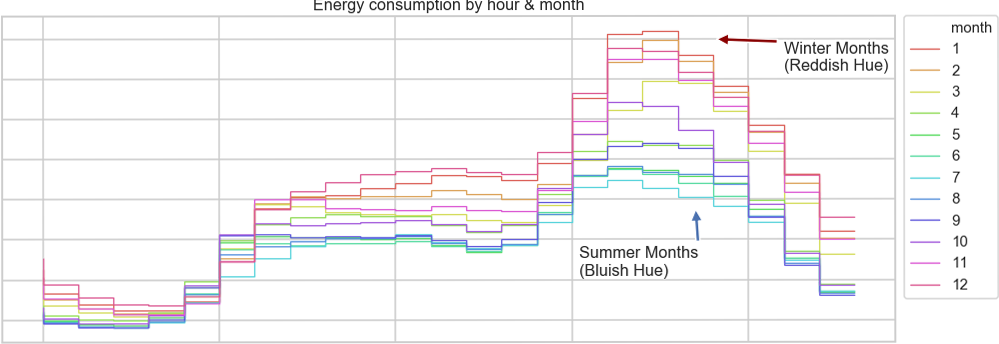
\includegraphics[width=16cm]{images/testimage1}
	\caption{This is an image}
	\label{fig:testimage1}
\end{figure*}

\begin{figure*}[!ht]
	\centering
	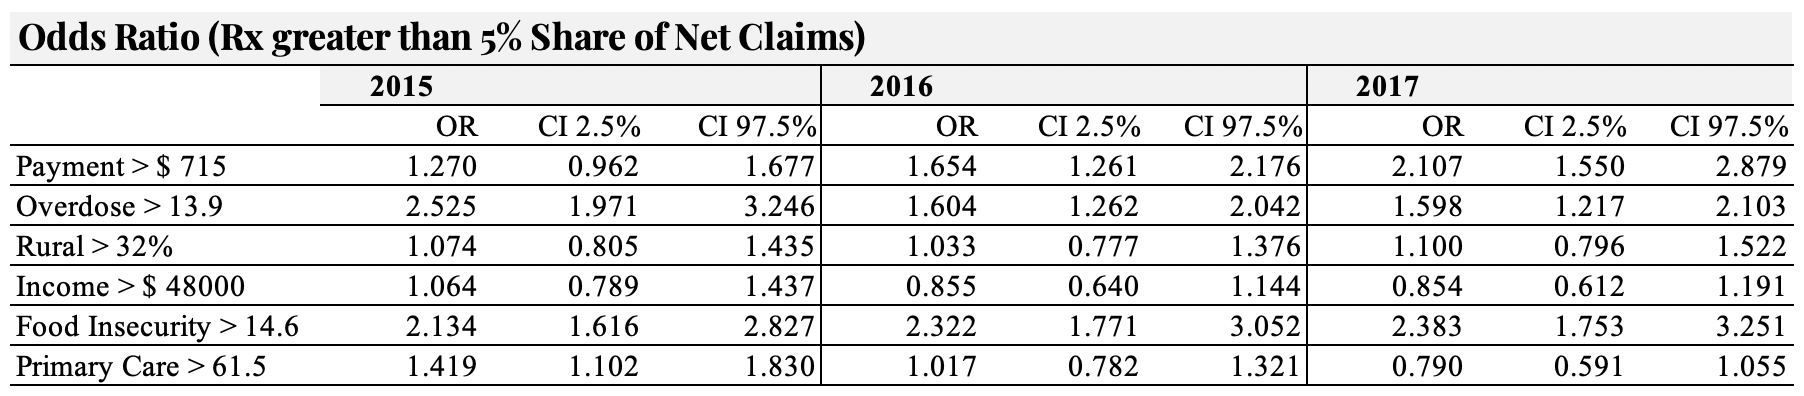
\includegraphics[width=16cm]{images/testimage2}
	%	\caption{Round 1 Blue Strategy to increase Market Share}
	\captionof{table}[This is a table shown as an image]{This is a table shown as an image}
	\label{fig:testimage2}
\end{figure*}

\begin{figure*}[!ht]
	\centering
	\subfloat[A floating image]{{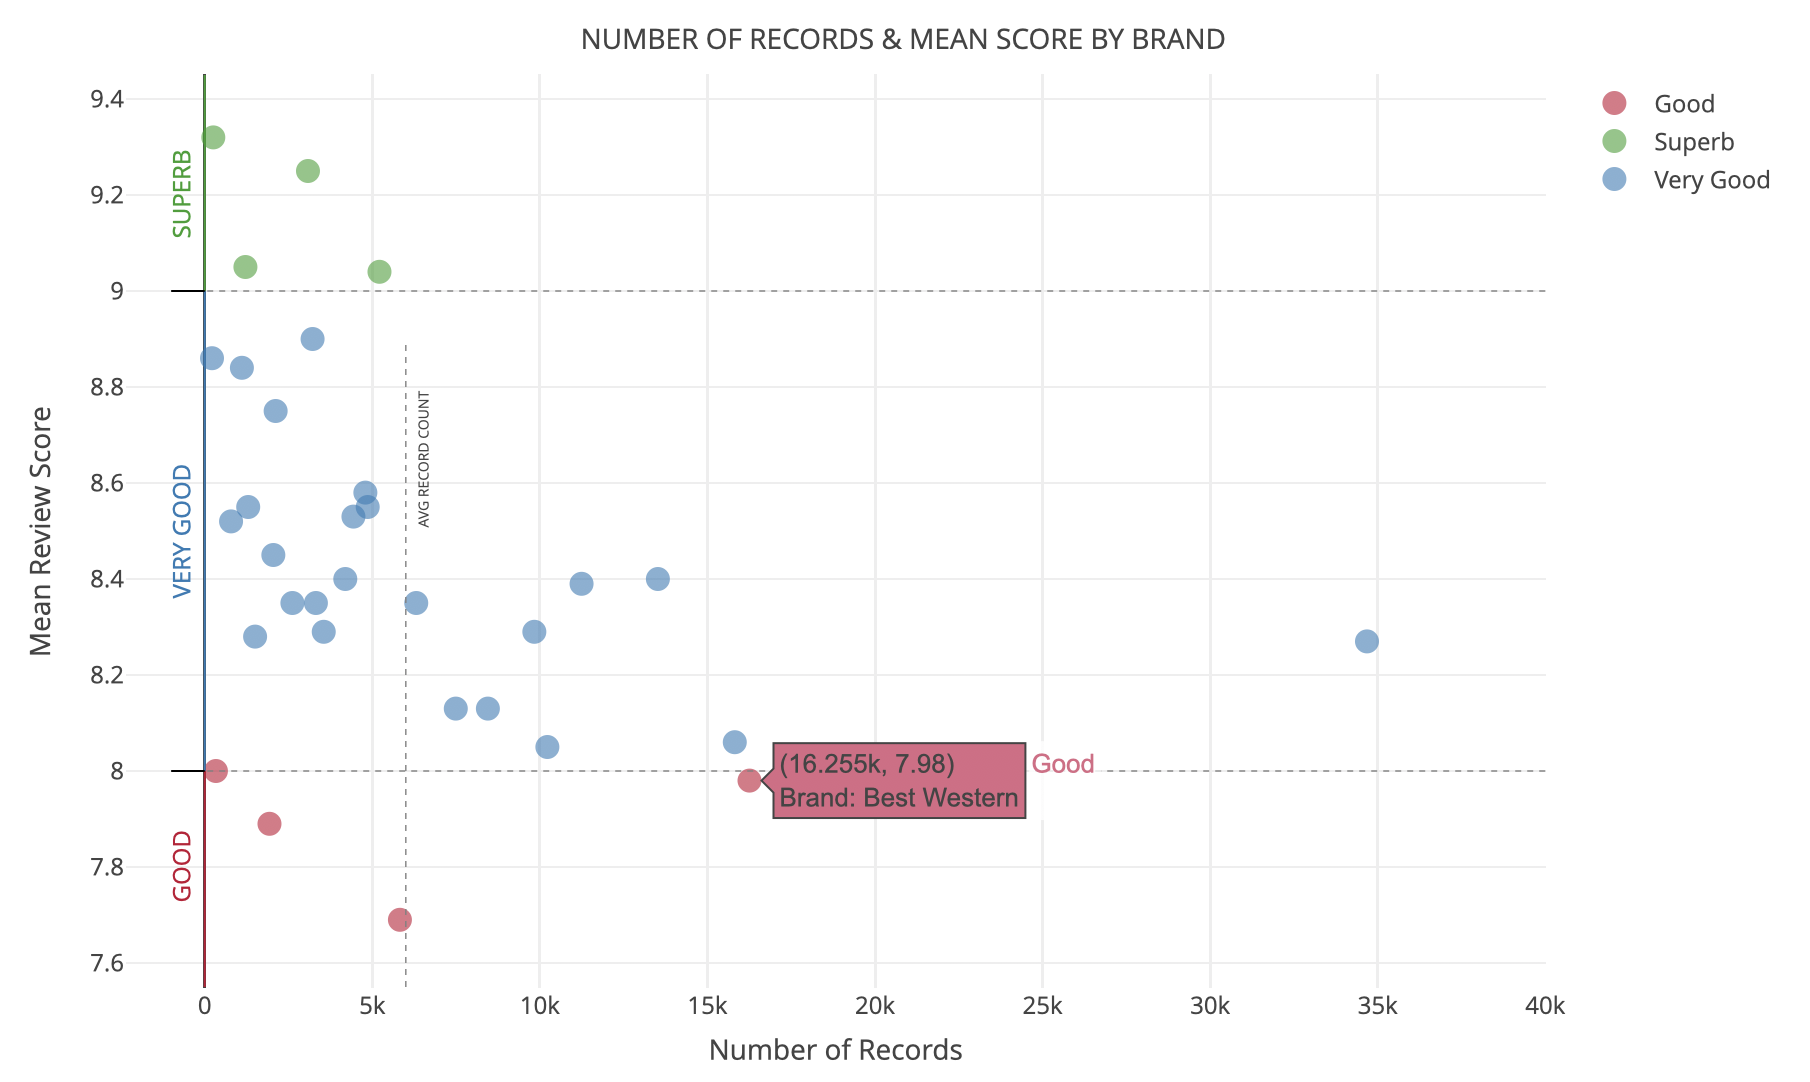
\includegraphics[width=7.2cm]{images/testimage3_1} }}%
	%	\qquad
	\subfloat[Another image ]{{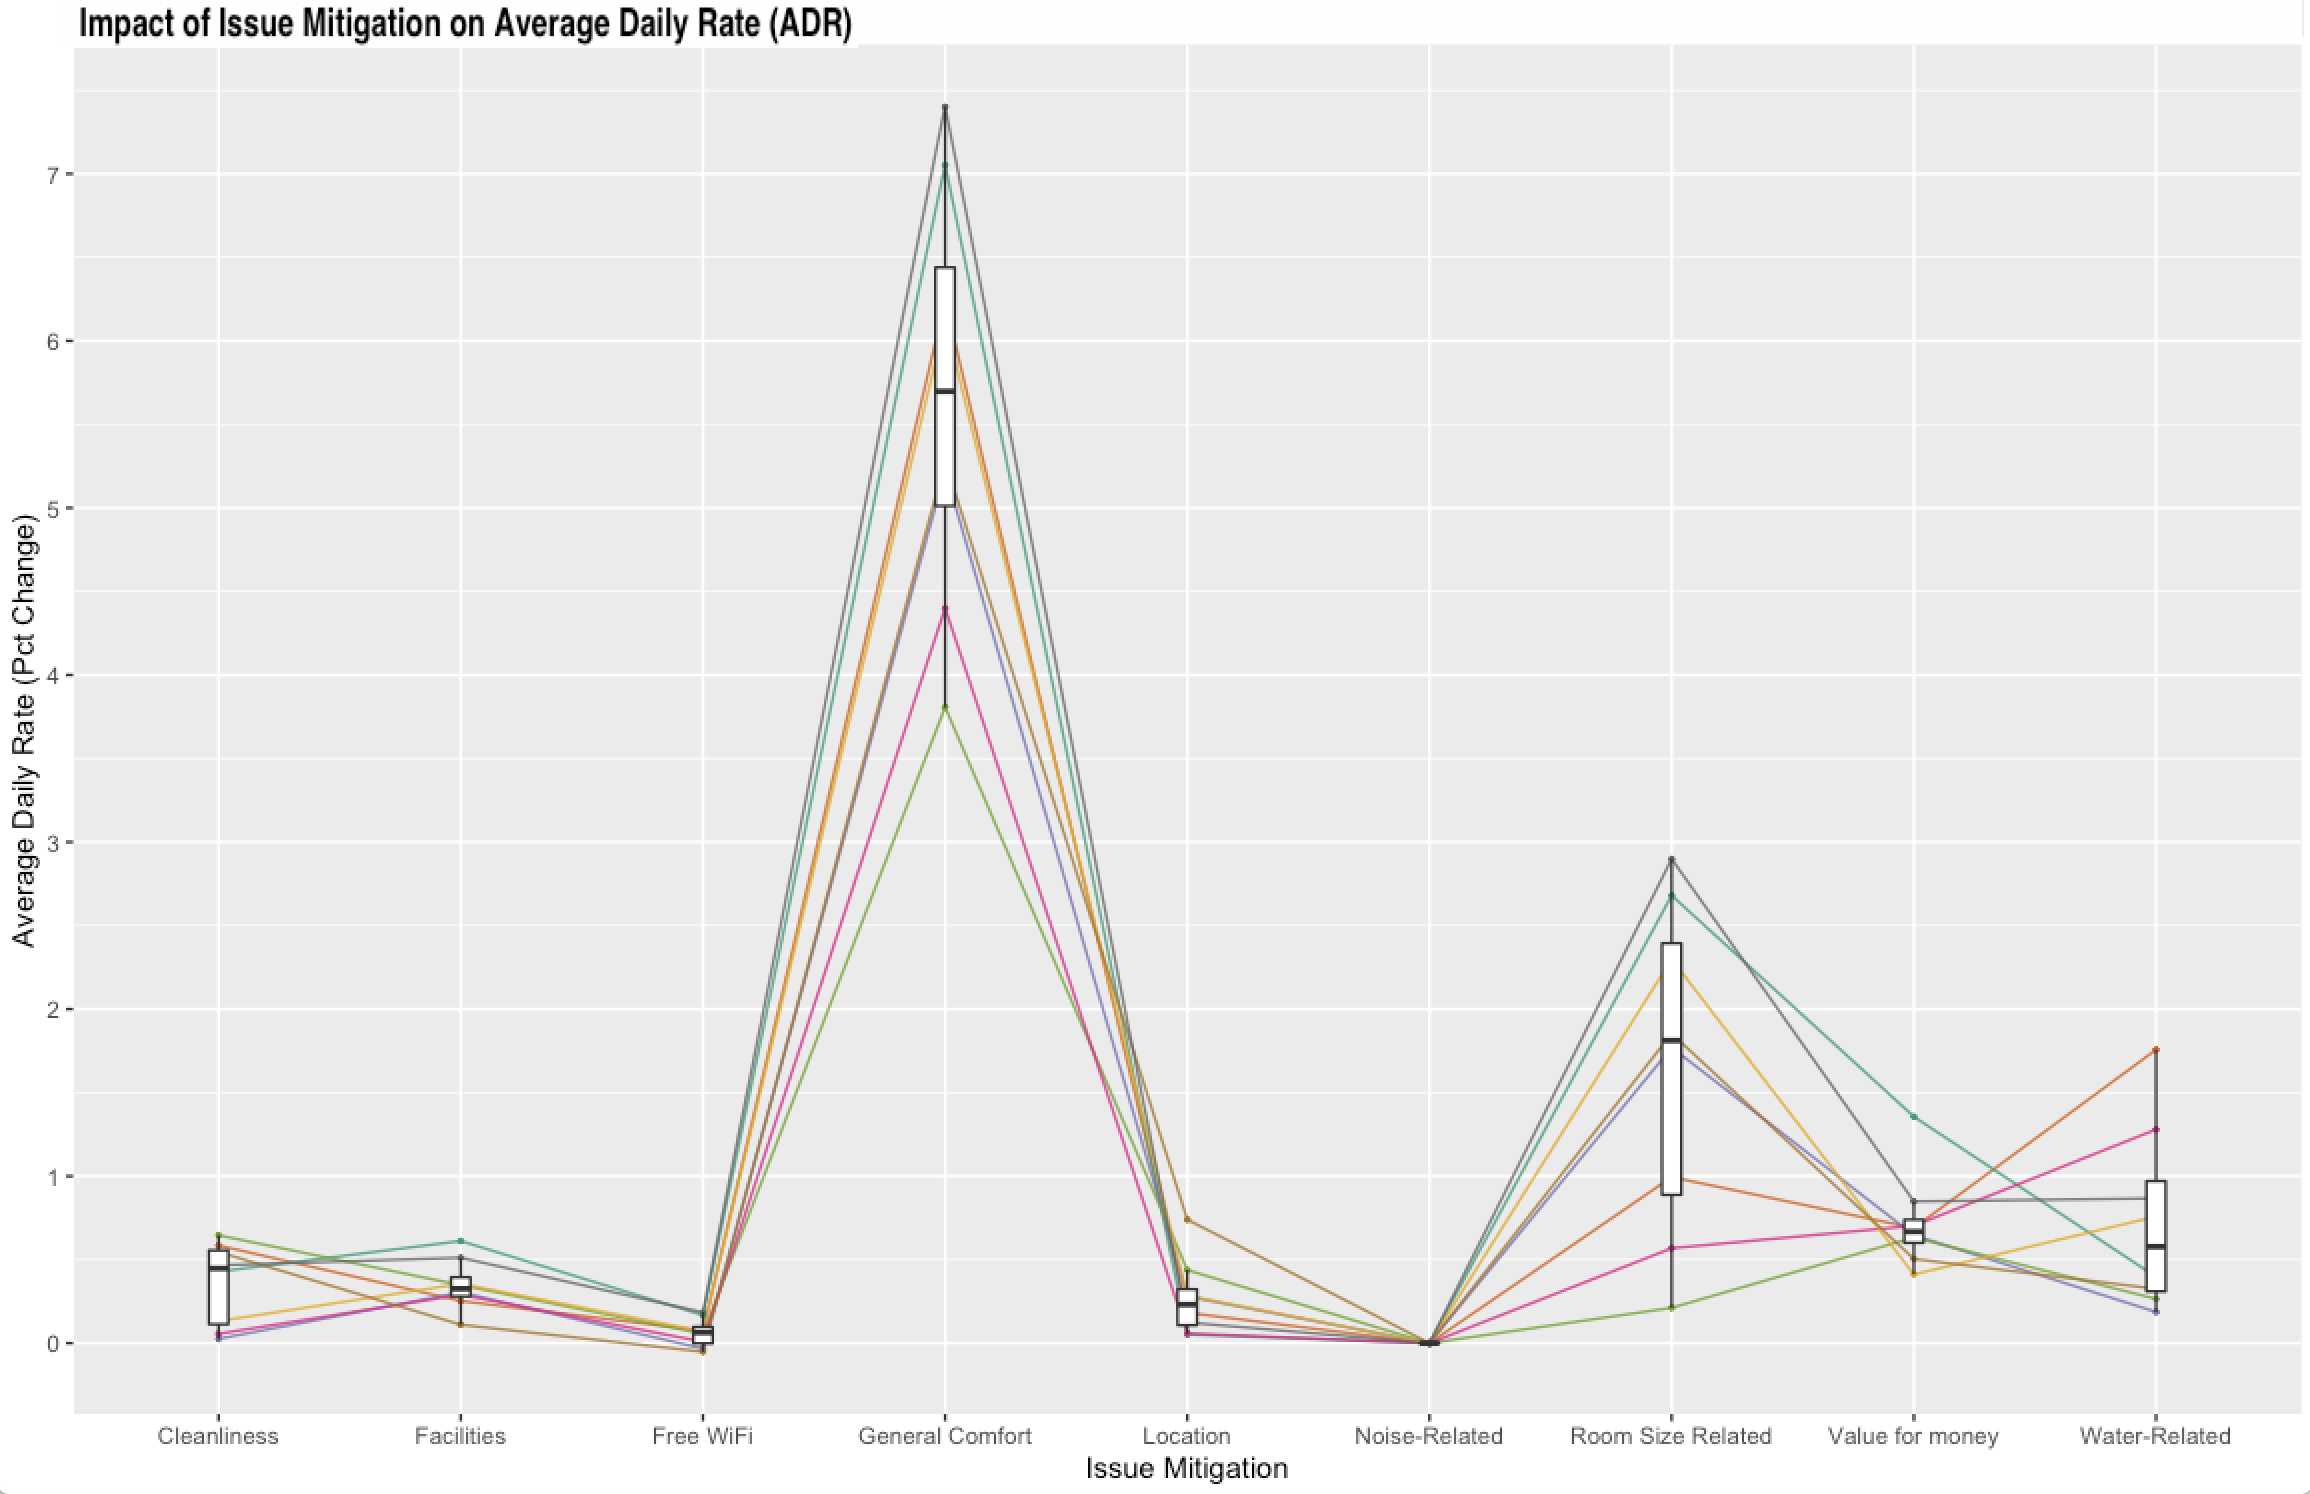
\includegraphics[width=7.2cm]{images/testimage3_2}}}%
	\caption{Floating Images}%
	\label{fig:floatimage}%
\end{figure*}


\subsection{Miscellaneous}

\subsubsection{Hyperlinks}
% HYPERLINK
\href{https://www.cnn.com}{A hyperlink to CNN.com}

% TO ADD A REFERENCE TO A SECTION
This is a section labelled as "sec1"
\label{sec:sec1}

This is a reference to the section sec1: \ref{sec:sec1}

\fbox{\begin{minipage}{43em}
		\textbf{Using fbox and minipage}\\
Text enclosed in a box
\end{minipage}}

% CODE
\subsubsection{Python Code Formatting}
\lstinputlisting[language=Python]{code/test.py}

\subsubsection{R Code Formatting}
\lstinputlisting[language=R]{code/test.R}

\subsubsection{Tables and Equations}

Examples with tables, caption centering, equations and aligned equations.

\begin{table}[!ht]
	\centering
	\captionsetup{justification=centering}
	\begin{tabular}{l|llrr}
		%		\hline
		\textbf{Model}            & \textbf{Parameter} & \textbf{Best Fit}              & \textbf{Train RMSE}             & \textbf{Test RMSE}               \\ \hline
		Linear Regression         & -                  & -                              & \rupee16,758,137 & \rupee57,778,006  \\ \hline
		Random GLM                & maxOrder           & maxInt.Order = 2        & \rupee15,551,472 & \rupee100,219,602 \\ \hline
		SVM RBF Kernel            & C, Sigma           & sigma = 26.76, C = 4     & \rupee17,075,271 & \rupee34,932,347  \\ \hline
		KNN                       & k                  & k = 5                          & \rupee12,255,888 & \rupee54,935,698  \\ \hline
		RandomForest              & mtry               & mtry = 2                       & \rupee8,724,815  & \rupee53,453,612  \\ \hline
		\rowcolor[HTML]{EFEFEF} 
		XGBoost & misc*              & max\_depth = 3, $\eta$ = 0.3, $\gamma$ = 0      & \rupee4,924,454  & \rupee65,211,901  \\ \hline
	\end{tabular}
	\caption{This is a table}
	\label{tab:state_pred}
\end{table}

Split Line in Equations
\begin{equation}
\begin{split}
\label{eqn:natsec}
ln(GVA_{Sector}) = \beta_1ln(SumOfLights)_{t}+\beta_2ln(SumElectricity)_t +\\ \beta_3ln(SumOfLightsSq)_{t} + \beta_4ln(Population)_{t} +
\alpha_i + u_{it}
\end{split}
\end{equation}

Aligned Equations
$$
\begin{aligned}
y_t &= 10.3009 -0.0042x_L - 0.0045x_B - 0.0032x_c -0.0046x_{d1} + \ldots + 0.0176x_{d6} + \eta_t \\
\eta_t &= 0.9146\eta_{t-1} + \epsilon_t -0.5015\epsilon_{t-1}\\
\epsilon_t &= \sim \text{NID}(0,0.003443)
\end{aligned}
$$

\subsubsection{Citations}
This template uses Bath BibTeX: \hyperlink{https://ctan.org/pkg/bath-bst?lang=en}{https://ctan.org/pkg/bath-bst?lang=en}

See: \hyperlink{https://github.com/alex-ball/bathbib/tree/master/bst}{https://github.com/alex-ball/bathbib/tree/master/bst}

This is a citation \citep{Elvidge_Baugh_Zhizhin_Hsu_Ghosh_2017} using \texttt{citep}.

This is a citation \cite{Tibshirani_1996} using \texttt{cite}

%TC:endignore
\pagebreak
\end{verbatim}
{\color{red} \rule{\linewidth}{0.5mm}}

\textcolor{red}{\textbf{FONT USAGE}}

The Arial font is recommended for the Individual Research Report. However, this needs to be installed manually as discussed in this document. For Overleaf, Helvetica has been used. If you are able to install Arial, comment the line \texttt{usepackage[scaled]\{helvet\}} and uncomment \texttt{usepackage\{uarial\}}.

{\color{red} \rule{\linewidth}{0.5mm}}

\textbf{FORMATTING AND PAGE NUMBERING CONVENTIONS USED}

\begin{itemize}
	\item Geometry
	\begin{itemize}
		\item left-hand margin of 4 cm;
		\item right-hand margin of 2.5cm (1 inch);
		\item top margin 2.5cm (1 inch);
		\item bottom margin 2.5cm (1 inch).
	\end{itemize}
	\begin{itemize}
		\item The Synopsis, Acknowledgements, List of Contents and Notation should be numbered with upper case Roman Numerals.
		\item The main text, starting with the first page of the first chapter (or Introduction) should be numbered, starting with page 1, using Arabic Numerals, through to the end of the references.
		\item \textbf{Appendices should be numbered using lower case Roman Numerals. -- Check to make sure this is what is needed. If not comment \texttt{\\pagenumbering\{roman\}} in template before Appendix}
	\end{itemize}
	\item Pages must be numbered at the bottom centre of the page.
	\item The title page should be blank.
\end{itemize}

\subsection{Prerequisites}

There are 2 primary pre-requisites: First, to install the Bath BibTeX style and second to install the Arial font. Note that if Arial cannot be installed, it may be possible to use Helvetica if the department agrees 

\textbf{1. Install the Bath BibTeX style (See Included Folder)}

\textbf{2. Install Font Arial}: See \hyperlink{https://www.tug.org/fonts/getnonfreefonts/}{https://www.tug.org/fonts/getnonfreefonts/} and 

\textbf{Notes from \hyperlink{https://tex.stackexchange.com/questions/37120/how-can-i-install-uarial-sty-on-a-mac}{Install uarial on a Mac} question on Stackexchange: }

The font can be easily installed via the script getnonfreefonts. It is available at tug.org: \hyperlink{http://www.tug.org/fonts/getnonfreefonts/}{getnonfreefonts}. I tried the installation of \hyperlink{http://www.tug.org/fonts/getnonfreefonts/install-getnonfreefonts}{getnonfreefonts} on my Mac.

\begin{itemize}
	\item Install MacTeX 
	\item Download the installation script. Open the terminal and go to the folder Download
	
	\texttt{cd Download}
	\item Run the installation: \texttt{sudo texlua install-getnonfreefonts}
	
	The installation finished and the scipts with their execute files getnonefreefonts and getnonfreefonts-sys are now located at \texttt{/usr/local/texlive/2011/bin/x86\_64-darwin/}
	
	\item Now you can run the script \texttt{sudo getnonfreefonts-sys -a}
\end{itemize}

\subsection{Images}
\begin{figure*}[!ht]
	\centering
	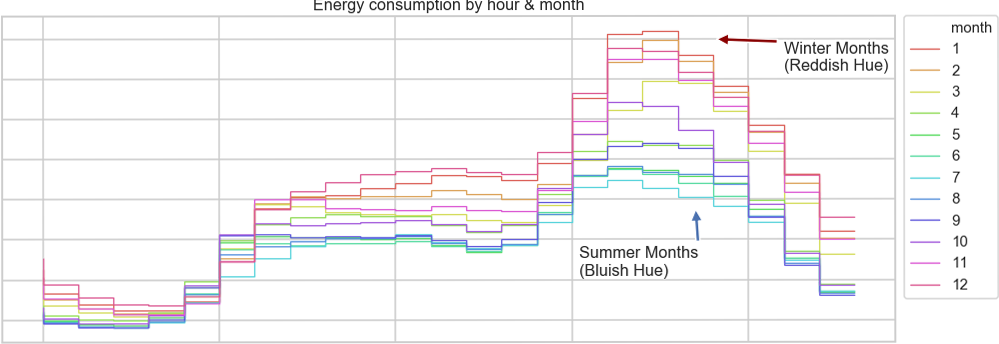
\includegraphics[width=16cm]{images/testimage1}
	\caption{This is an image}
	\label{fig:testimage1}
\end{figure*}

\begin{figure*}[!ht]
	\centering
	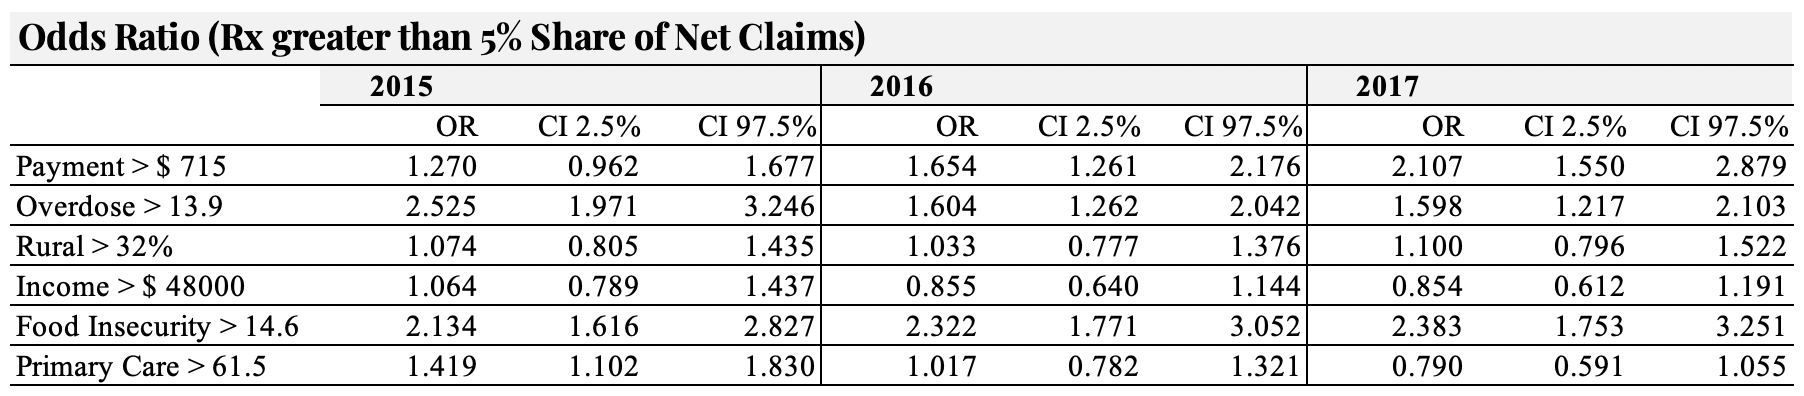
\includegraphics[width=16cm]{images/testimage2}
	%	\caption{Round 1 Blue Strategy to increase Market Share}
	\captionof{table}[This is a table shown as an image]{This is a table shown as an image}
	\label{fig:testimage2}
\end{figure*}

\begin{figure*}[!ht]
	\centering
	\subfloat[A floating image]{{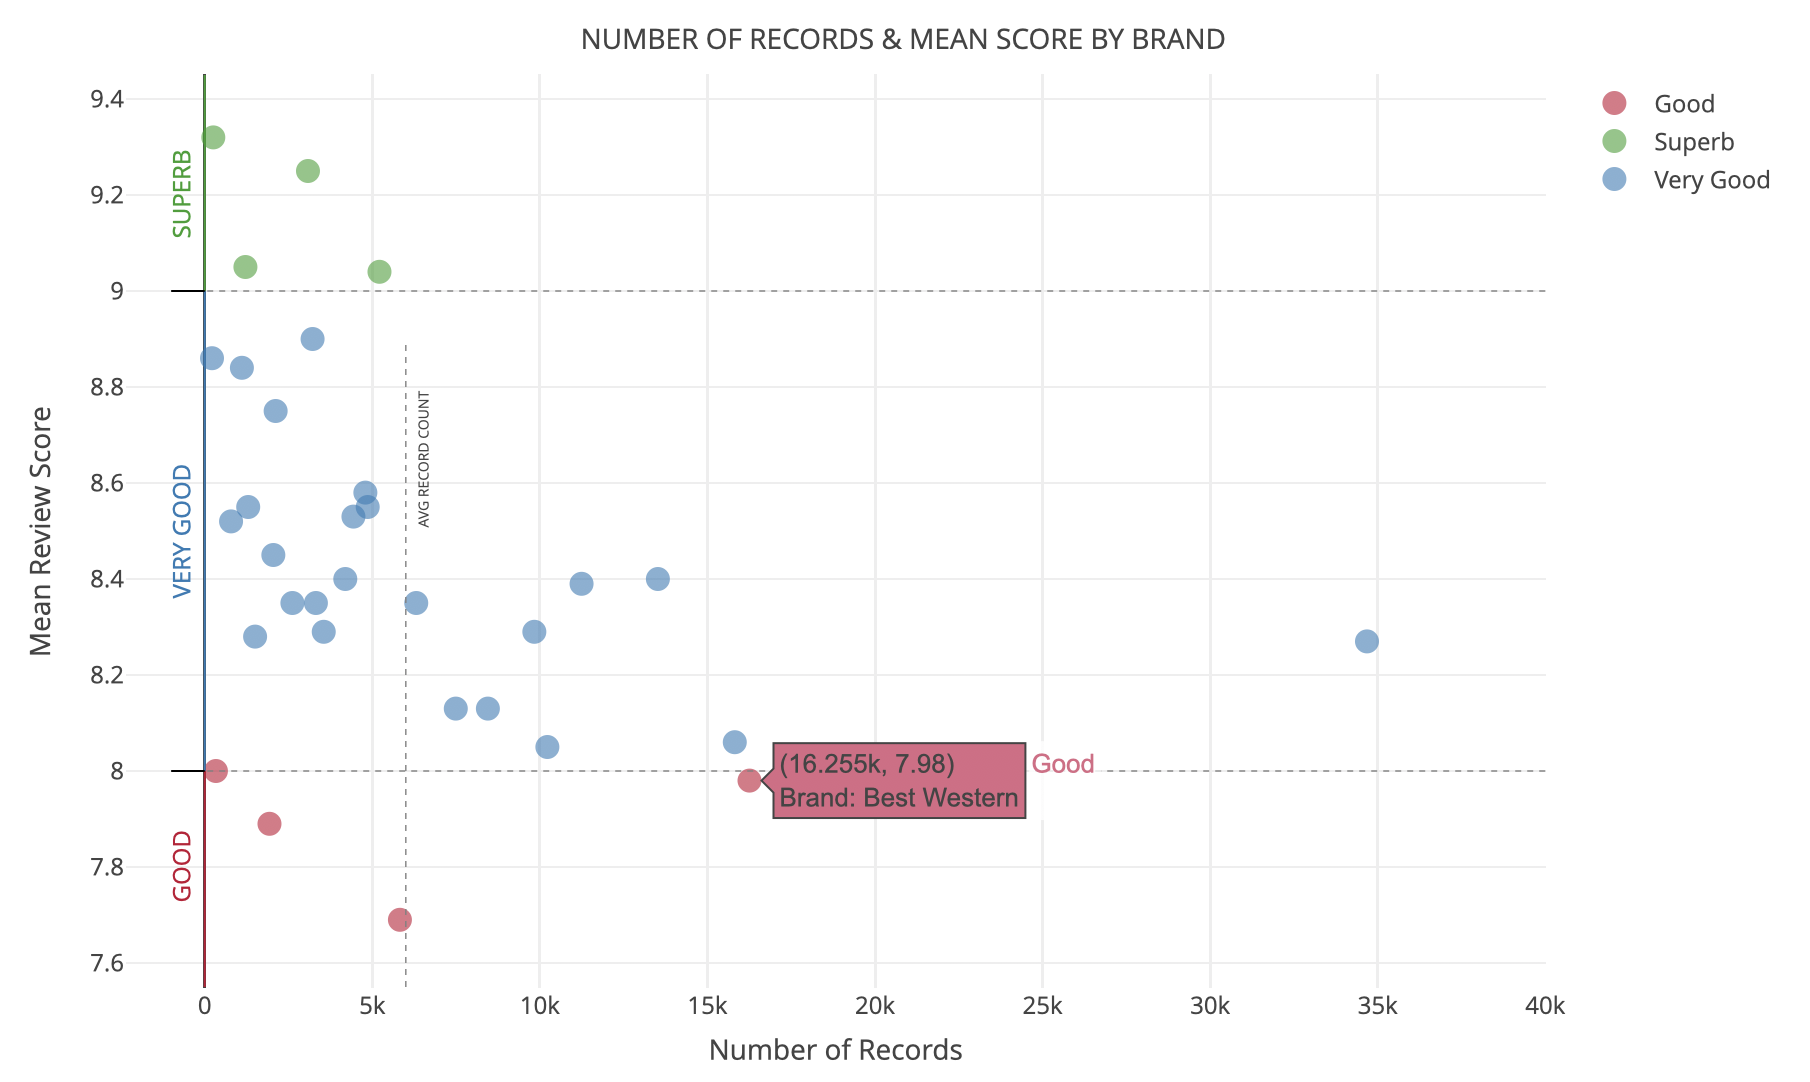
\includegraphics[width=7.2cm]{images/testimage3_1} }}%
	%	\qquad
	\subfloat[Another image ]{{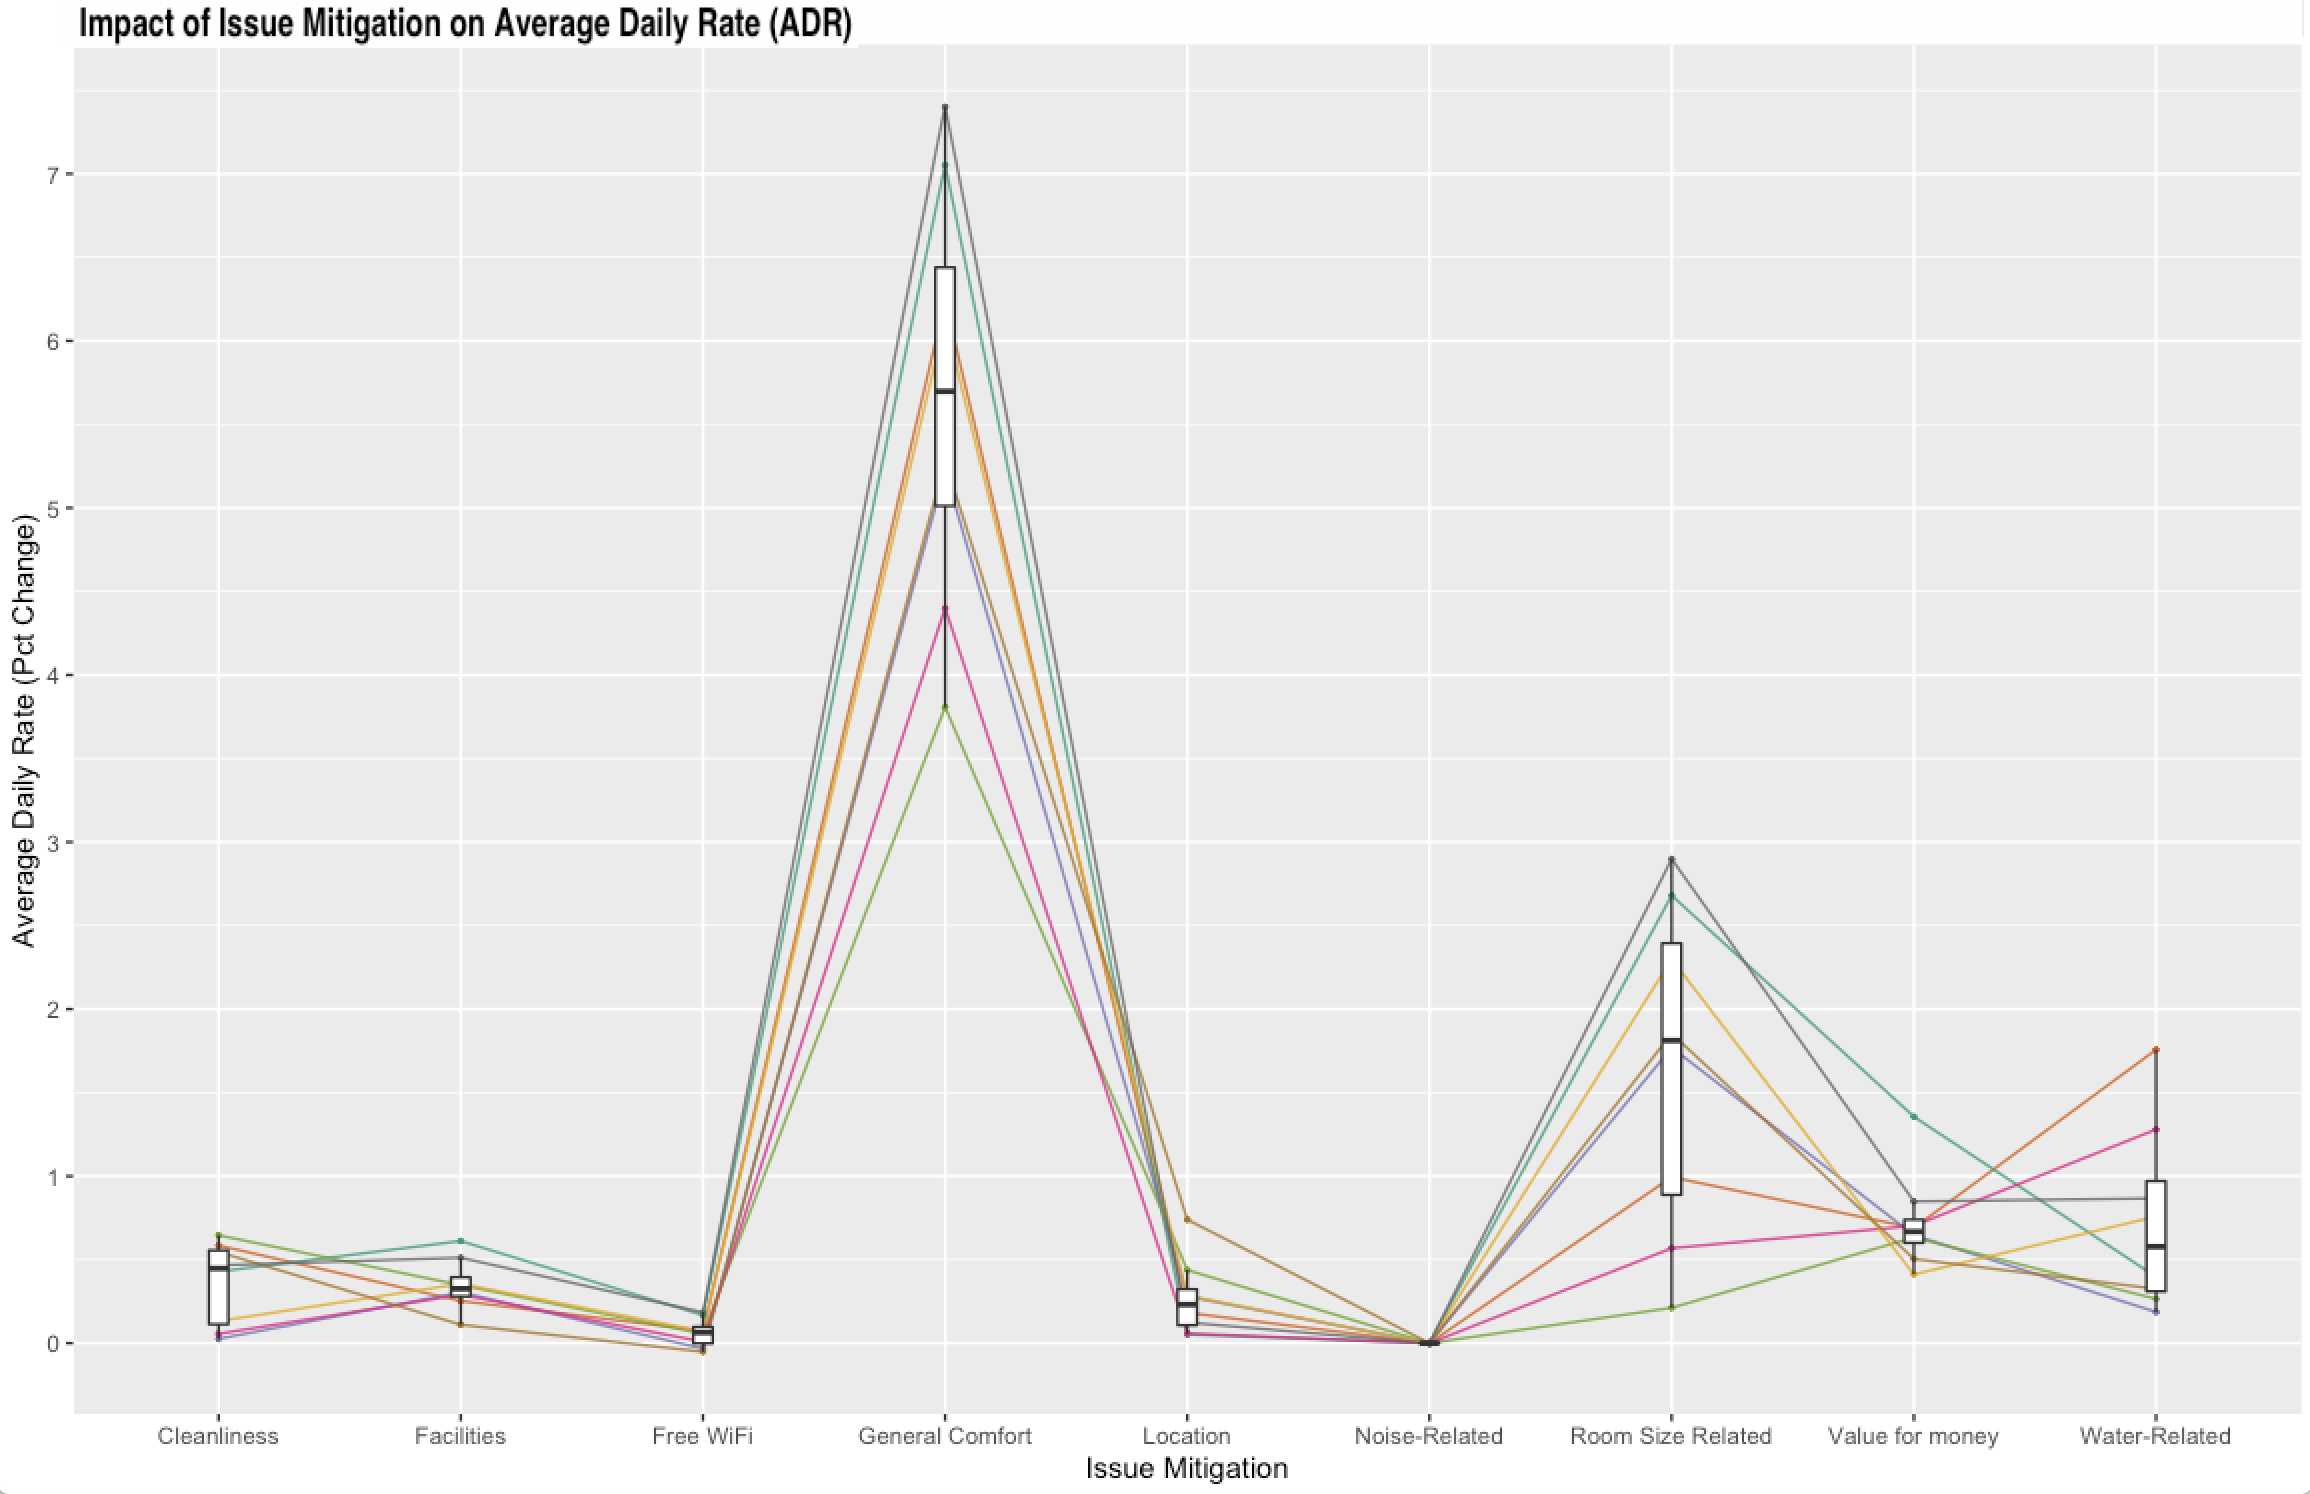
\includegraphics[width=7.2cm]{images/testimage3_2}}}%
	\caption{Floating Images}%
	\label{fig:floatimage}%
\end{figure*}


\subsection{Miscellaneous}

\subsubsection{Hyperlinks}
% HYPERLINK
\href{https://www.cnn.com}{A hyperlink to CNN.com}

% TO ADD A REFERENCE TO A SECTION
This is a section labelled as "sec1"
\label{sec:sec1}

This is a reference to the section sec1: \ref{sec:sec1}

\fbox{\begin{minipage}{43em}
		\textbf{Using fbox and minipage}\\
Text enclosed in a box
\end{minipage}}

% CODE
\subsubsection{Python Code Formatting}
\lstinputlisting[language=Python]{code/test.py}

\subsubsection{R Code Formatting}
\lstinputlisting[language=R]{code/test.R}

\subsubsection{Tables and Equations}

Examples with tables, caption centering, equations and aligned equations.

\begin{table}[!ht]
	\centering
	\captionsetup{justification=centering}
	\begin{tabular}{l|llrr}
		%		\hline
		\textbf{Model}            & \textbf{Parameter} & \textbf{Best Fit}              & \textbf{Train RMSE}             & \textbf{Test RMSE}               \\ \hline
		Linear Regression         & -                  & -                              & \rupee16,758,137 & \rupee57,778,006  \\ \hline
		Random GLM                & maxOrder           & maxInt.Order = 2        & \rupee15,551,472 & \rupee100,219,602 \\ \hline
		SVM RBF Kernel            & C, Sigma           & sigma = 26.76, C = 4     & \rupee17,075,271 & \rupee34,932,347  \\ \hline
		KNN                       & k                  & k = 5                          & \rupee12,255,888 & \rupee54,935,698  \\ \hline
		RandomForest              & mtry               & mtry = 2                       & \rupee8,724,815  & \rupee53,453,612  \\ \hline
		\rowcolor[HTML]{EFEFEF} 
		XGBoost & misc*              & max\_depth = 3, $\eta$ = 0.3, $\gamma$ = 0      & \rupee4,924,454  & \rupee65,211,901  \\ \hline
	\end{tabular}
	\caption{This is a table}
	\label{tab:state_pred}
\end{table}

Split Line in Equations
\begin{equation}
\begin{split}
\label{eqn:natsec}
ln(GVA_{Sector}) = \beta_1ln(SumOfLights)_{t}+\beta_2ln(SumElectricity)_t +\\ \beta_3ln(SumOfLightsSq)_{t} + \beta_4ln(Population)_{t} +
\alpha_i + u_{it}
\end{split}
\end{equation}

Aligned Equations
$$
\begin{aligned}
y_t &= 10.3009 -0.0042x_L - 0.0045x_B - 0.0032x_c -0.0046x_{d1} + \ldots + 0.0176x_{d6} + \eta_t \\
\eta_t &= 0.9146\eta_{t-1} + \epsilon_t -0.5015\epsilon_{t-1}\\
\epsilon_t &= \sim \text{NID}(0,0.003443)
\end{aligned}
$$

\subsubsection{Citations}
This template uses Bath BibTeX: \hyperlink{https://ctan.org/pkg/bath-bst?lang=en}{https://ctan.org/pkg/bath-bst?lang=en}

See: \hyperlink{https://github.com/alex-ball/bathbib/tree/master/bst}{https://github.com/alex-ball/bathbib/tree/master/bst}

This is a citation \citep{Elvidge_Baugh_Zhizhin_Hsu_Ghosh_2017} using \texttt{citep}.

This is a citation \cite{Tibshirani_1996} using \texttt{cite}

%TC:endignore
\pagebreak
\end{verbatim}
{\color{red} \rule{\linewidth}{0.5mm}}

\textcolor{red}{\textbf{FONT USAGE}}

The Arial font is recommended for the Individual Research Report. However, this needs to be installed manually as discussed in this document. For Overleaf, Helvetica has been used. If you are able to install Arial, comment the line \texttt{usepackage[scaled]\{helvet\}} and uncomment \texttt{usepackage\{uarial\}}.

{\color{red} \rule{\linewidth}{0.5mm}}

\textbf{FORMATTING AND PAGE NUMBERING CONVENTIONS USED}

\begin{itemize}
	\item Geometry
	\begin{itemize}
		\item left-hand margin of 4 cm;
		\item right-hand margin of 2.5cm (1 inch);
		\item top margin 2.5cm (1 inch);
		\item bottom margin 2.5cm (1 inch).
	\end{itemize}
	\begin{itemize}
		\item The Synopsis, Acknowledgements, List of Contents and Notation should be numbered with upper case Roman Numerals.
		\item The main text, starting with the first page of the first chapter (or Introduction) should be numbered, starting with page 1, using Arabic Numerals, through to the end of the references.
		\item \textbf{Appendices should be numbered using lower case Roman Numerals. -- Check to make sure this is what is needed. If not comment \texttt{\\pagenumbering\{roman\}} in template before Appendix}
	\end{itemize}
	\item Pages must be numbered at the bottom centre of the page.
	\item The title page should be blank.
\end{itemize}

\subsection{Prerequisites}

There are 2 primary pre-requisites: First, to install the Bath BibTeX style and second to install the Arial font. Note that if Arial cannot be installed, it may be possible to use Helvetica if the department agrees 

\textbf{1. Install the Bath BibTeX style (See Included Folder)}

\textbf{2. Install Font Arial}: See \hyperlink{https://www.tug.org/fonts/getnonfreefonts/}{https://www.tug.org/fonts/getnonfreefonts/} and 

\textbf{Notes from \hyperlink{https://tex.stackexchange.com/questions/37120/how-can-i-install-uarial-sty-on-a-mac}{Install uarial on a Mac} question on Stackexchange: }

The font can be easily installed via the script getnonfreefonts. It is available at tug.org: \hyperlink{http://www.tug.org/fonts/getnonfreefonts/}{getnonfreefonts}. I tried the installation of \hyperlink{http://www.tug.org/fonts/getnonfreefonts/install-getnonfreefonts}{getnonfreefonts} on my Mac.

\begin{itemize}
	\item Install MacTeX 
	\item Download the installation script. Open the terminal and go to the folder Download
	
	\texttt{cd Download}
	\item Run the installation: \texttt{sudo texlua install-getnonfreefonts}
	
	The installation finished and the scipts with their execute files getnonefreefonts and getnonfreefonts-sys are now located at \texttt{/usr/local/texlive/2011/bin/x86\_64-darwin/}
	
	\item Now you can run the script \texttt{sudo getnonfreefonts-sys -a}
\end{itemize}

\subsection{Images}
\begin{figure*}[!ht]
	\centering
	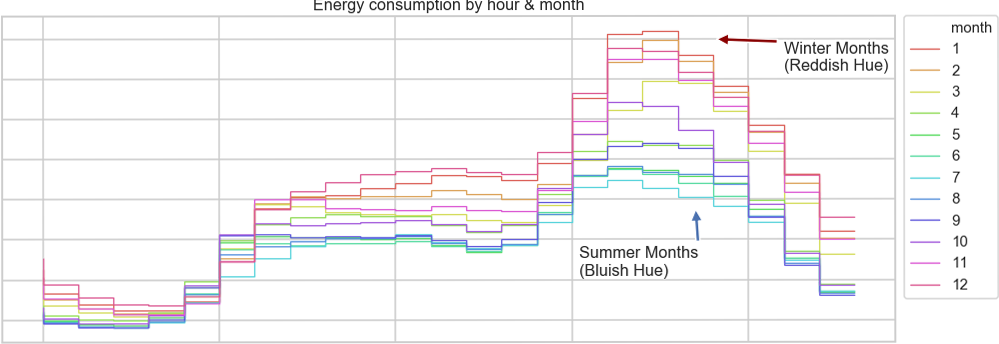
\includegraphics[width=16cm]{images/testimage1}
	\caption{This is an image}
	\label{fig:testimage1}
\end{figure*}

\begin{figure*}[!ht]
	\centering
	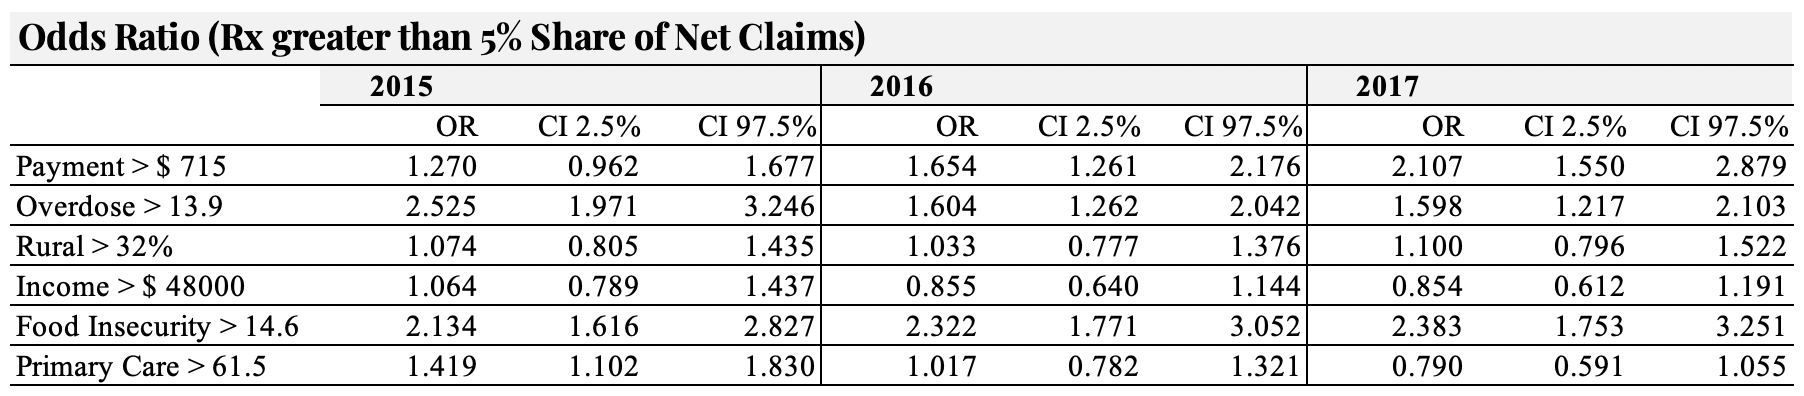
\includegraphics[width=16cm]{images/testimage2}
	%	\caption{Round 1 Blue Strategy to increase Market Share}
	\captionof{table}[This is a table shown as an image]{This is a table shown as an image}
	\label{fig:testimage2}
\end{figure*}

\begin{figure*}[!ht]
	\centering
	\subfloat[A floating image]{{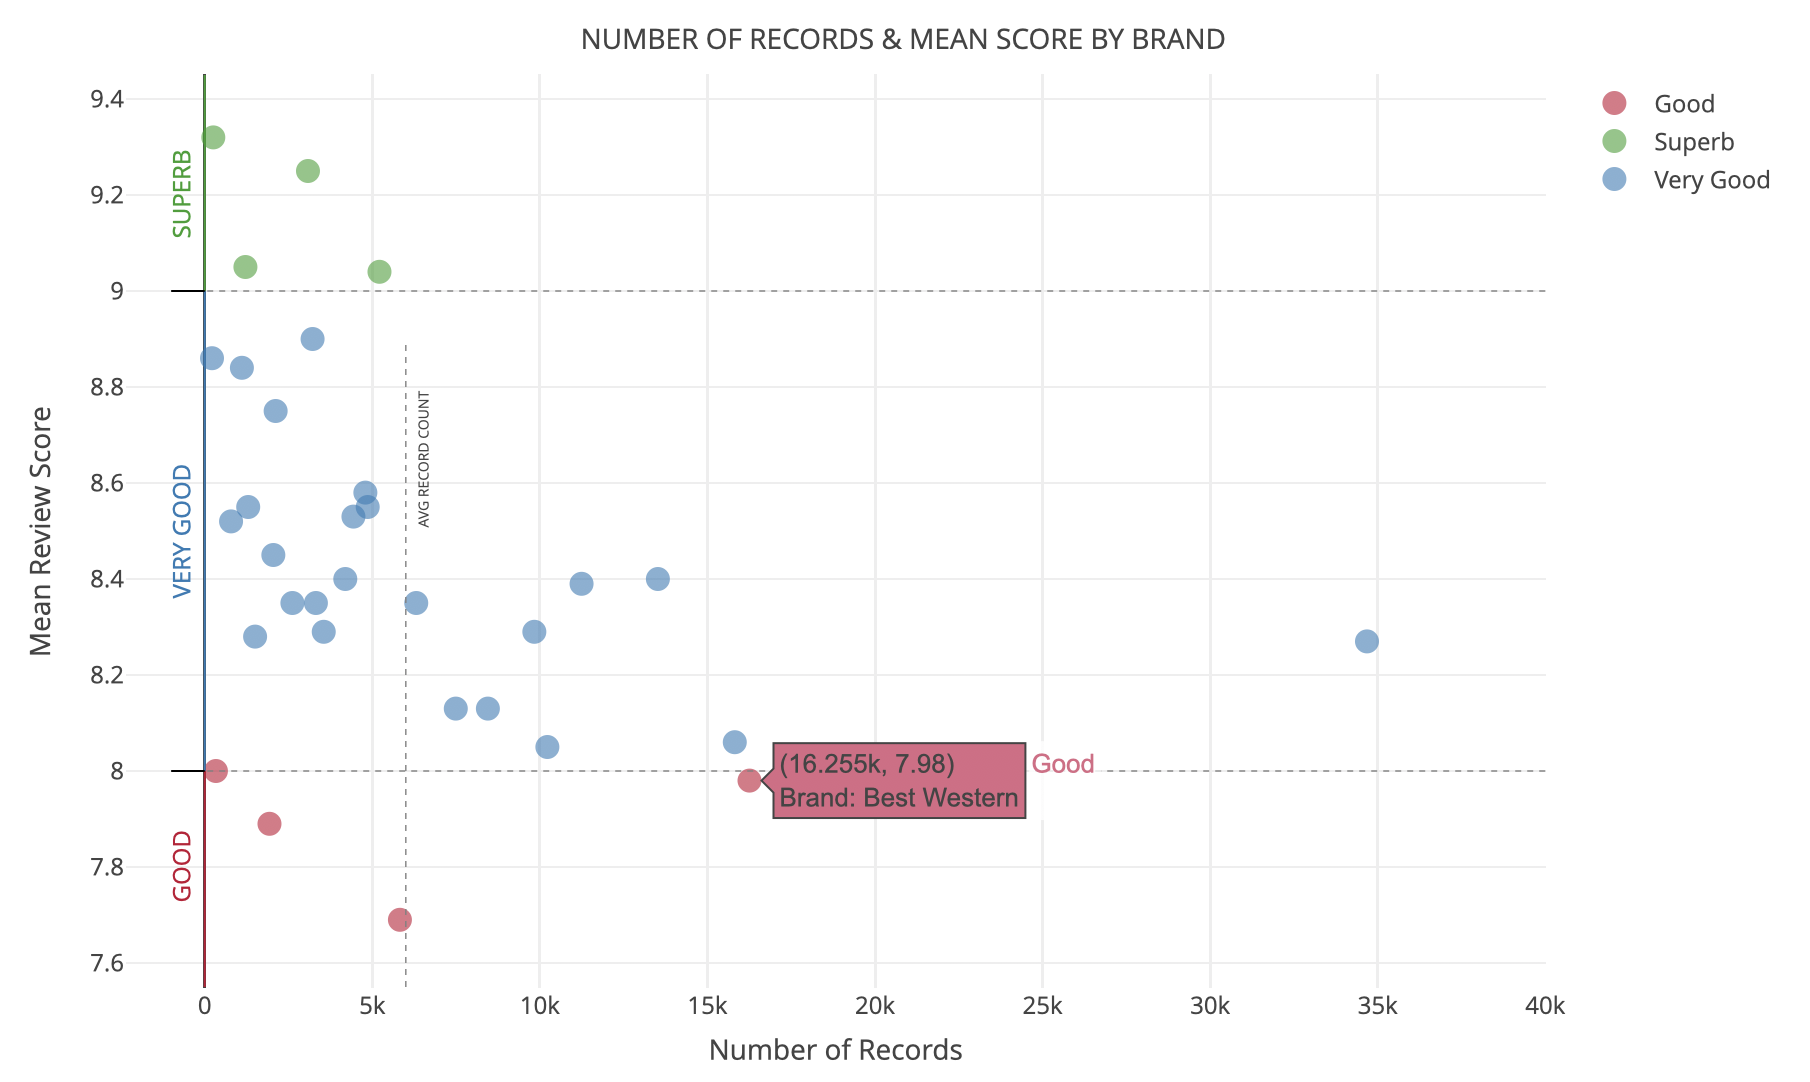
\includegraphics[width=7.2cm]{images/testimage3_1} }}%
	%	\qquad
	\subfloat[Another image ]{{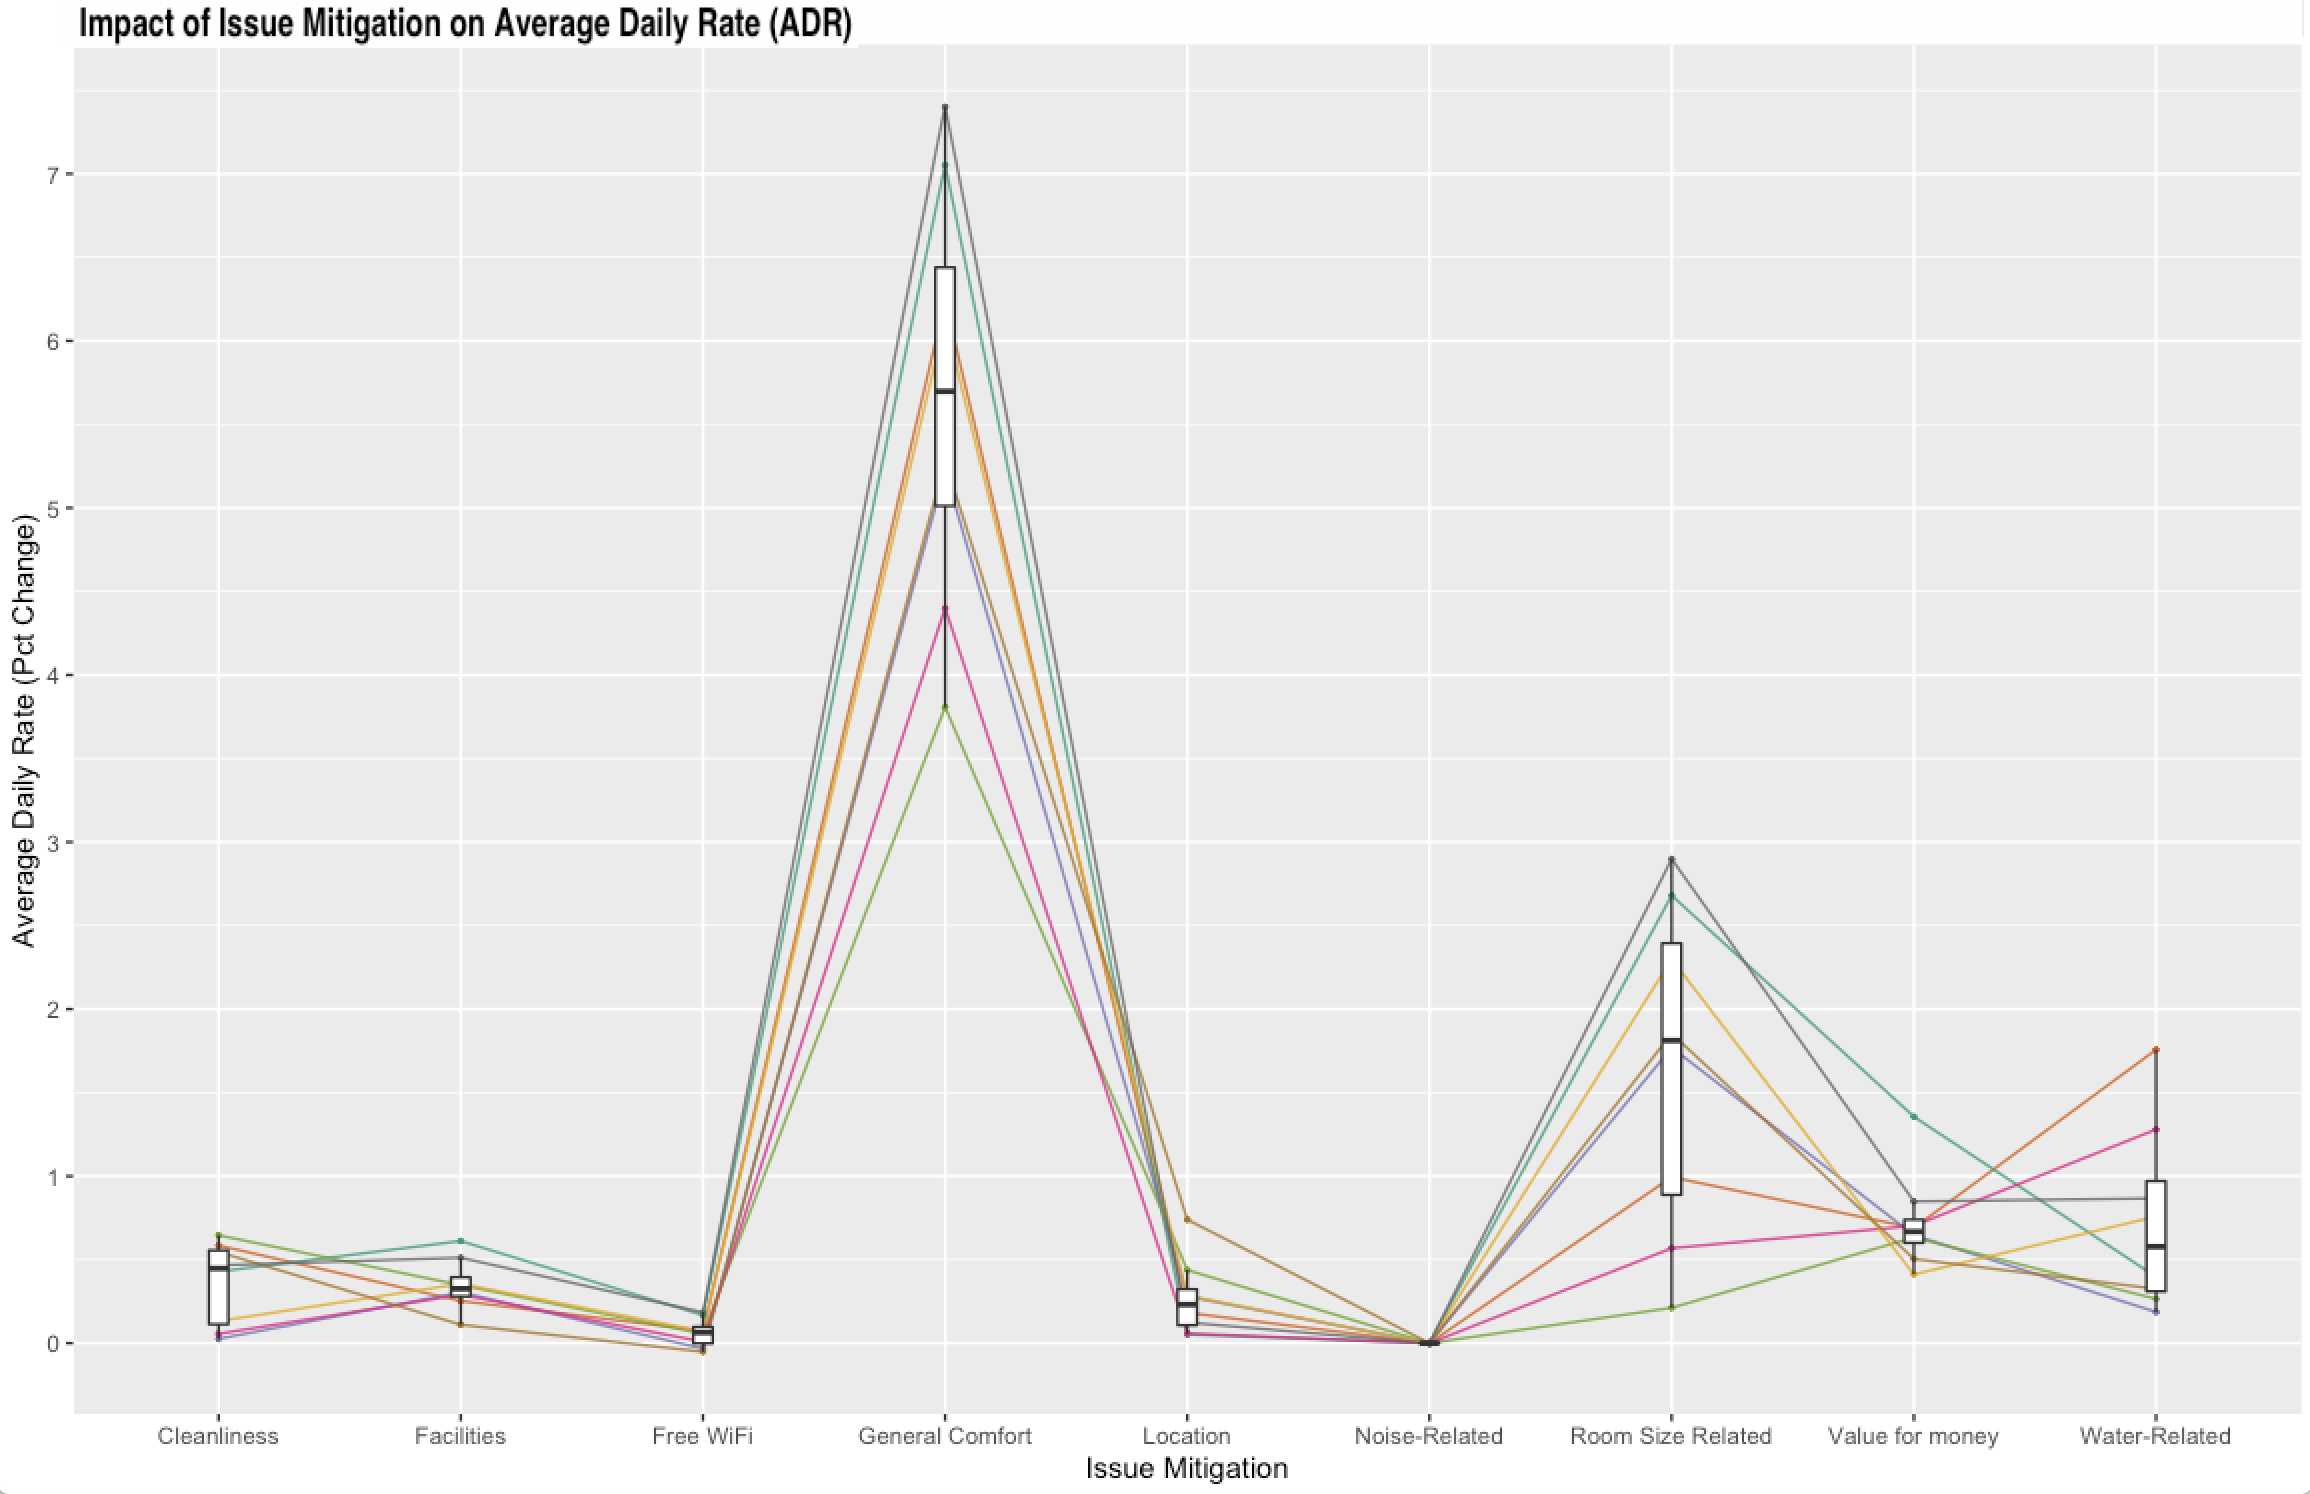
\includegraphics[width=7.2cm]{images/testimage3_2}}}%
	\caption{Floating Images}%
	\label{fig:floatimage}%
\end{figure*}


\subsection{Miscellaneous}

\subsubsection{Hyperlinks}
% HYPERLINK
\href{https://www.cnn.com}{A hyperlink to CNN.com}

% TO ADD A REFERENCE TO A SECTION
This is a section labelled as "sec1"
\label{sec:sec1}

This is a reference to the section sec1: \ref{sec:sec1}

\fbox{\begin{minipage}{43em}
		\textbf{Using fbox and minipage}\\
Text enclosed in a box
\end{minipage}}

% CODE
\subsubsection{Python Code Formatting}
\lstinputlisting[language=Python]{code/test.py}

\subsubsection{R Code Formatting}
\lstinputlisting[language=R]{code/test.R}

\subsubsection{Tables and Equations}

Examples with tables, caption centering, equations and aligned equations.

\begin{table}[!ht]
	\centering
	\captionsetup{justification=centering}
	\begin{tabular}{l|llrr}
		%		\hline
		\textbf{Model}            & \textbf{Parameter} & \textbf{Best Fit}              & \textbf{Train RMSE}             & \textbf{Test RMSE}               \\ \hline
		Linear Regression         & -                  & -                              & \rupee16,758,137 & \rupee57,778,006  \\ \hline
		Random GLM                & maxOrder           & maxInt.Order = 2        & \rupee15,551,472 & \rupee100,219,602 \\ \hline
		SVM RBF Kernel            & C, Sigma           & sigma = 26.76, C = 4     & \rupee17,075,271 & \rupee34,932,347  \\ \hline
		KNN                       & k                  & k = 5                          & \rupee12,255,888 & \rupee54,935,698  \\ \hline
		RandomForest              & mtry               & mtry = 2                       & \rupee8,724,815  & \rupee53,453,612  \\ \hline
		\rowcolor[HTML]{EFEFEF} 
		XGBoost & misc*              & max\_depth = 3, $\eta$ = 0.3, $\gamma$ = 0      & \rupee4,924,454  & \rupee65,211,901  \\ \hline
	\end{tabular}
	\caption{This is a table}
	\label{tab:state_pred}
\end{table}

Split Line in Equations
\begin{equation}
\begin{split}
\label{eqn:natsec}
ln(GVA_{Sector}) = \beta_1ln(SumOfLights)_{t}+\beta_2ln(SumElectricity)_t +\\ \beta_3ln(SumOfLightsSq)_{t} + \beta_4ln(Population)_{t} +
\alpha_i + u_{it}
\end{split}
\end{equation}

Aligned Equations
$$
\begin{aligned}
y_t &= 10.3009 -0.0042x_L - 0.0045x_B - 0.0032x_c -0.0046x_{d1} + \ldots + 0.0176x_{d6} + \eta_t \\
\eta_t &= 0.9146\eta_{t-1} + \epsilon_t -0.5015\epsilon_{t-1}\\
\epsilon_t &= \sim \text{NID}(0,0.003443)
\end{aligned}
$$

\subsubsection{Citations}
This template uses Bath BibTeX: \hyperlink{https://ctan.org/pkg/bath-bst?lang=en}{https://ctan.org/pkg/bath-bst?lang=en}

See: \hyperlink{https://github.com/alex-ball/bathbib/tree/master/bst}{https://github.com/alex-ball/bathbib/tree/master/bst}

This is a citation \citep{Elvidge_Baugh_Zhizhin_Hsu_Ghosh_2017} using \texttt{citep}.

This is a citation \cite{Tibshirani_1996} using \texttt{cite}

%TC:endignore
%\pagebreak

%\section*{Synopsis}
%\textbf{MAXIMUM 250 WORDS}

%\include{synopsis.tex}


\pagebreak

%\section*{Acknowledgments}
%\include{Acknowledgments.tex}
%\blindtext
%\pagebreak


%\section*{EXAMPLEEEEEEEEEEEEEEEEES}
%%TC:ignore

\iffalse
- Lisette, Menghua, Emily, David: submodels + references
- Write text about submodels
- Elias: Why SD + consistency between intro/methods
    - intro: examples
    - methods: arguments
    + model structure + hypothesis (once we have received feedback)
- Emily(1st), Menghua(2nd): introduction

Deadline: 25-02 morning


Possible expansions future:
- include children in costs of illness and care for them by elderly (children have a higher chance of getting infected)

\fi




\subsection*{Examples how to cite}

Here I give some examples how to cite:
\cite{moore_campylobacter_2005}
\parencite{moore_campylobacter_2005} 
\textcite{moore_campylobacter_2005}
\citeauthor{moore_campylobacter_2005}
\citetitle{moore_campylobacter_2005}

\subsection*{How to add an image}

\begin{figure*}[!ht]
	\centering
	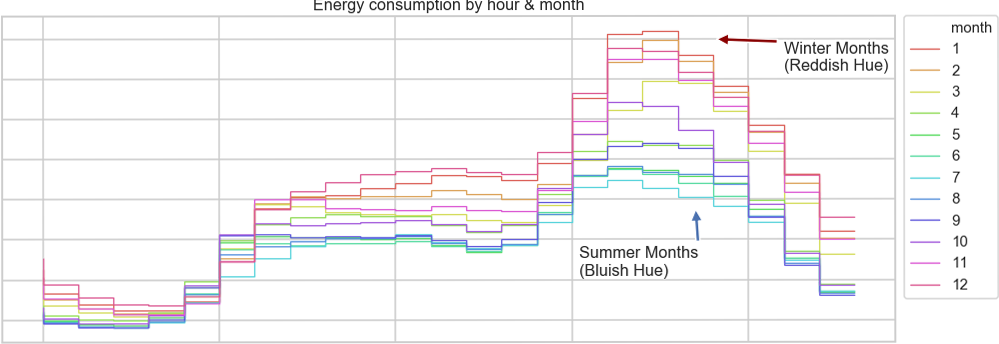
\includegraphics[width=\textwidth]{images/testimage1}
	\caption{This is an image}
	\label{fig:testimage1}
\end{figure*}

\begin{figure*}[!ht]
	\centering
	\subfloat[A floating image]{{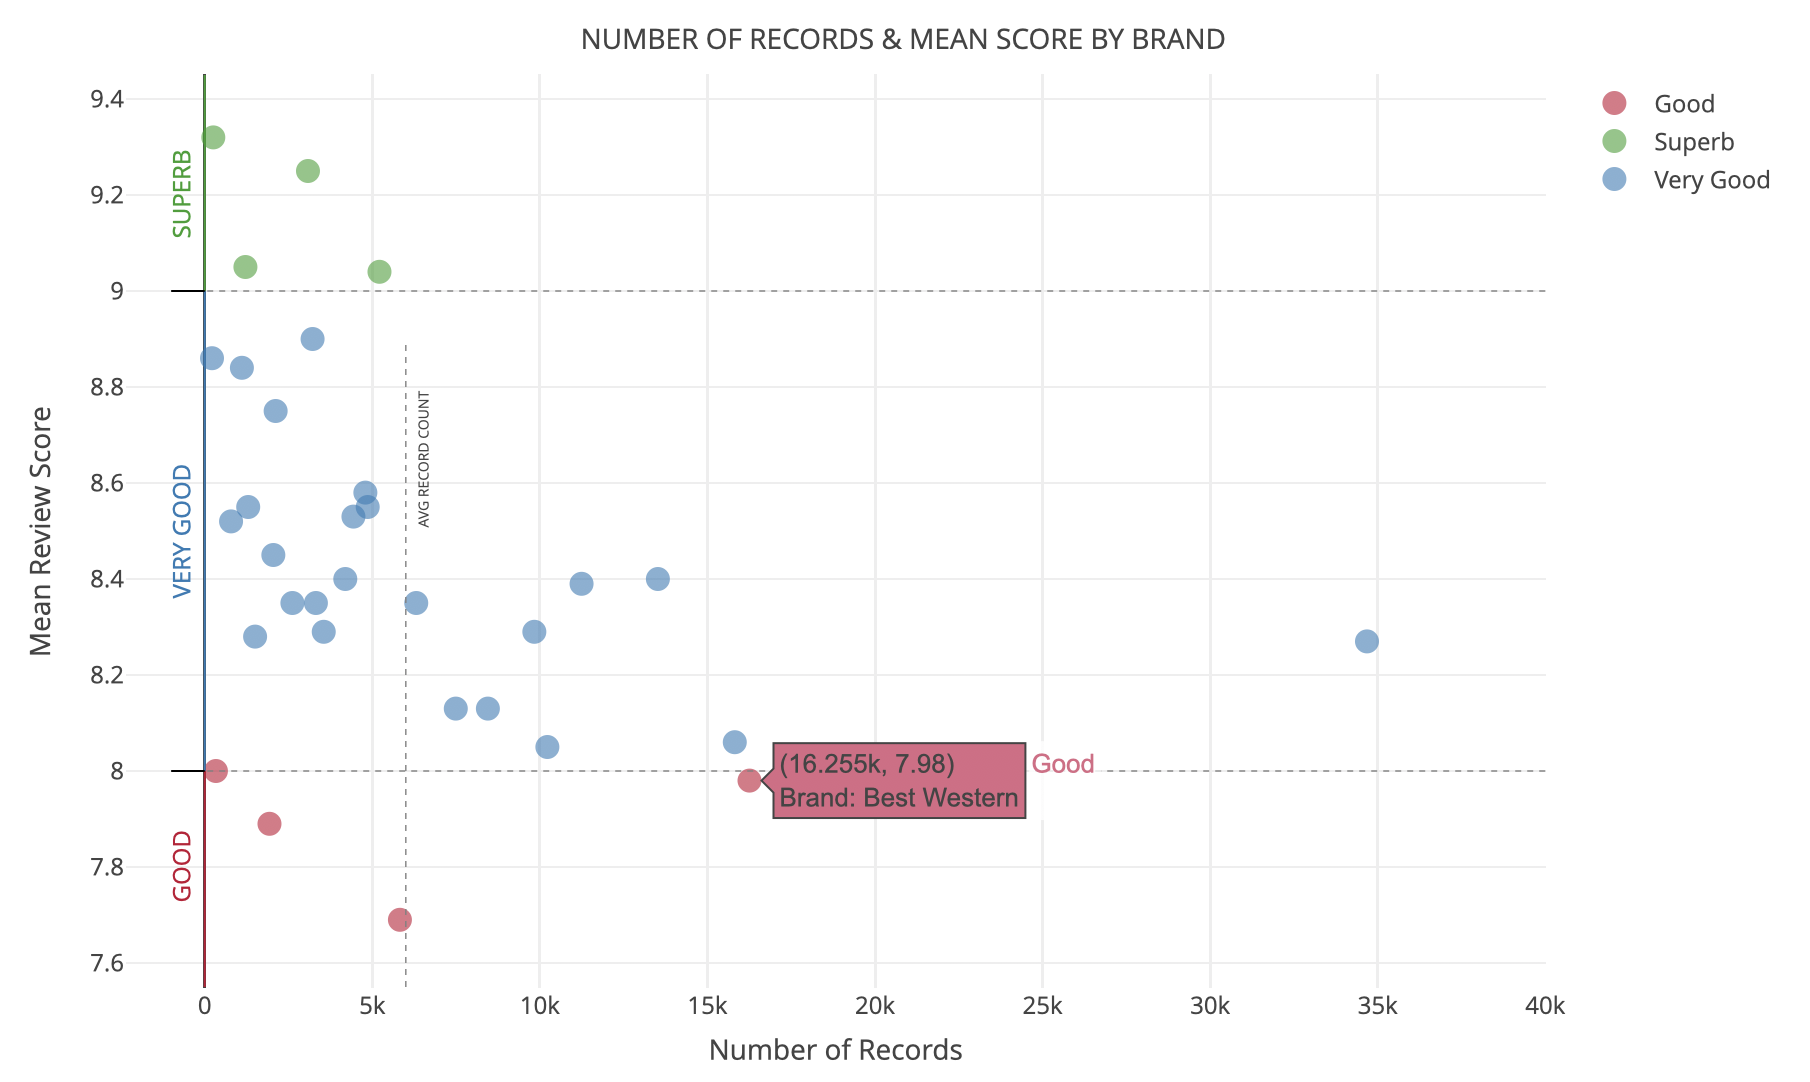
\includegraphics[width=0.45\textwidth]{images/testimage3_1} }}%
	%	\qquad
	\subfloat[Another image ]{{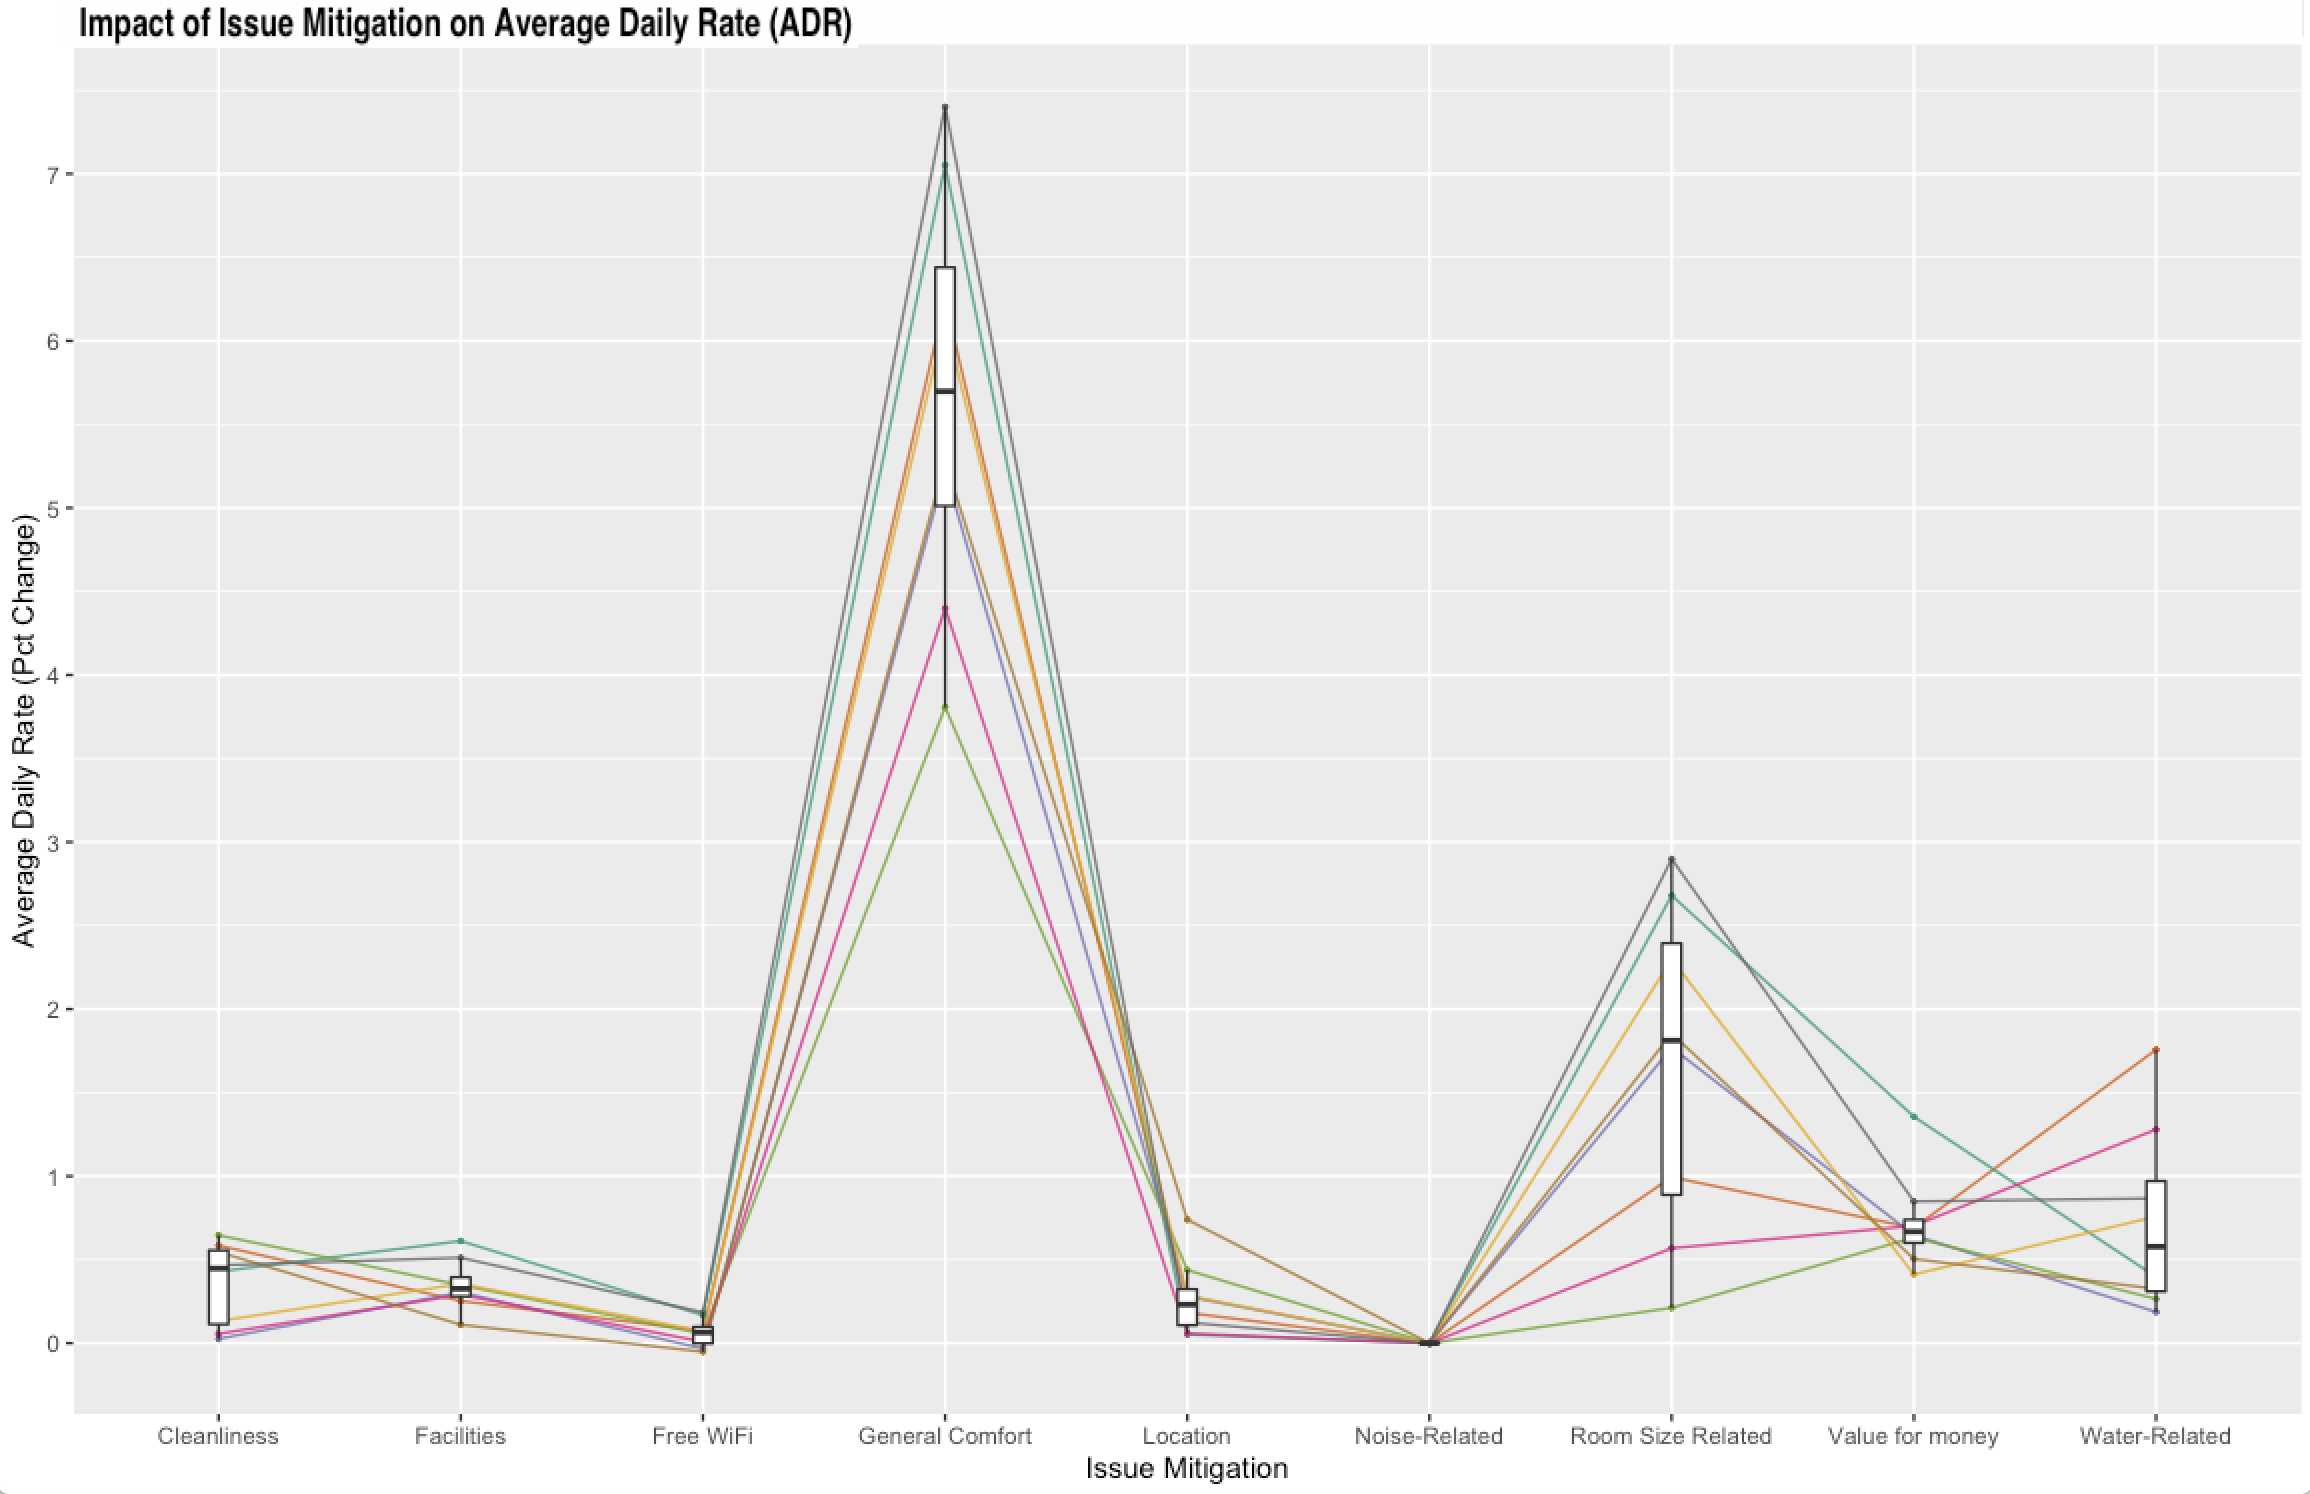
\includegraphics[width=0.45\textwidth]{images/testimage3_2}}}%
	\caption{Floating Images}%
	\label{fig:floatimage}%
\end{figure*}


\subsection*{How to equation}

Split Line in Equations
\begin{equation}
\begin{split}
\label{eqn:natsec}
ln(GVA_{Sector}) = \beta_1ln(SumOfLights)_{t}+\beta_2ln(SumElectricity)_t +\\ \beta_3ln(SumOfLightsSq)_{t} + \beta_4ln(Population)_{t} +
\alpha_i + u_{it}
\end{split}
\end{equation}

Aligned Equations
$$
\begin{aligned}
y_t &= 10.3009 -0.0042x_L - 0.0045x_B - 0.0032x_c -0.0046x_{d1} + \ldots + 0.0176x_{d6} + \eta_t \\
\eta_t &= 0.9146\eta_{t-1} + \epsilon_t -0.5015\epsilon_{t-1}\\
\epsilon_t &= \sim \text{NID}(0,0.003443)
\end{aligned}
$$

{\Huge \textcolor{pink}{FEEL FREE TO ASK ME QUESTIONS - Z}}

%TC:endignore

\section*{Abstract}
%TC:ignore

\begin{itemize}
% From rubric, recommended format is: situation, complication, question/aim, approach, answer, recommendation.
    \item Situation: \textit{Campylobacter} affects close to 100.000 people a year in the Netherlands and costs the Dutch economy millions of euros and more in accumulated costs from chronic diseases. 
    
    \item Complication: \textit{Campylobacter} is spread through transmissions routes that are tied in with certain factors, such as the number of flies. 
    
    \item Aim: Thus, this report we aim to understand if climate change will result in more \textit{Campylobacter} infections and increase the hidden burden on the environment and whether or not policy levers might impact the case numbers and cost of illness. 
    \item Method: These impacts and causal relationships are modelled using system dynamics principles with VenSim PLE. 
    
    \item Key Results: It was found that 
    
    \item Conclusion: 
\end{itemize}

%TC:endignore

\pagebreak

\section*{Glossary}
\begin{table}[ht!]
\begin{tabular}{lm{45em}}
 \textbf{Campylobacteriosis} & The infectious disease caused by bacteria of the genus \emph{Campylobacter} \\
  \textbf{Disease vector} & Biological agent that carries and/or transmits \textit{Campylobacter} between other organisms. \\
  \textbf{KPI} & Key Performance Indicator which is a way to measure an objective.
\end{tabular}
\end{table}

\pagebreak

%\section*{List of Contents}
\tableofcontents
\pagebreak
\listoffigures
\listoftables
\pagebreak
\newpage
%\section{Notation}
%\textbf{IF APPLICABLE}
%%\include{Acknowledgments.tex}


\cleardoublepage\pagenumbering{arabic}

\section{Introduction}
\iffalse
1.	Establish field  -> Z
    a.	Societal relevance
2.	Outline problem in the field (Elias)
    a.	Scientific relevance
3.	Present solution to problem in the field
    a.	Problem statement/research question -> Z
    b.	Explain relevance of simulation method (Elias) considering the problem
4.	Reading guide -> Z

Target: 1000 words\
♫♪.ılılıll|̲̅̅●̲̅̅|̲̅̅=̲̅̅|̲̅̅●̲̅̅|llılılı.♫♪
\fi

%1a
Although Campylobacter is regarded as a primal cause of foodborne diseases in Europe \parencite{european_food_safety_authority_european_2019}
, its (possible) economic impact has been understudied. The \citeauthor{european_food_safety_authority_campylobacter_nodate} estimates that the burden on health care and the loss of productivity caused by the pathogen in the European Union to be around \euro{} 2.4 billion a year. %It has been shown that E. Coli burdens the health care of the United States, and costs billions of dollars \textcite{russo_medical_2003}

%2a
Campylobacteriosis has been identified to be  the most common cause of bacterial gastro-enteritis in the developed world.



This project is part of the course EPA1341 Advanced System Dynamics. The project will expand upon prior research conducted on the topic of \textit{Campylobacter}, a bacteria often found in poultry which causes diarrhoeal disease in humans. Adding to existing research, the economic impact of policy measures aimed to prevent the spread of  \textit{Campylobacter} and the effect climate change has will be explored. In order to analyse different policy measures, the programming environment of Vensim is used. 


\pagebreak

\section{Methods}
\label{ch:methods}
\subsection{Model explanation}
\textcolor{red}{Add a short introduction to introduce the subsections}
\subsection{How is System Dynamics used?}
An important aspect to system dynamics models are the aforementioned accumulations, delays and feed-backs. Accumulations, more commonly referred to as stock variables refer to some value material or entities within a system. Through flow or rate variables stocks dynamically change over time, leading to the aforementioned delay and feed-back effects \parencite{sterman_system_2001}. To build the sub-models for the study on \textit{Campylobacter} appropriate variables had to be chosen to represent these features. In the case of, infected populations of humans and flocks would act modelled as stocks, whilst various transmission routes provide flow variables between them. This naturally produces delays, as it takes time for the disease to spread, symptoms to surface and potential hospitalisation. Feed-back loops will also arise as \textit{Campylobacter}, as the number of contaminated chicken flocks, causes more spread of \textit{Campylobacter} in the environment, and in turn the more \textit{Campylobacter} in the environment, the more easily chicken flocks are infected. Furthermore the model was subdivided into multiple subsystems, which will be explained in the following paragraphs. 

%1.	Explain basics of SD
 %   a.	Basics of SD
  %  b.	Examples from literature to clarify and justify modelling choices given problem in the field
%2.	Conceptualisation
  %  a.	Depict aggregate model structure
   % b.	Describe dynamic hypothesis

\subsection{Conceptualisation}
The model will focus on the economic impacts and health care costs associated with \textit{Campylobacter}-contaminated chicken meat. The dynamic hypothesis includes three KPIs that will be examined to answer the research question: 
\begin{itemize}
    % \item Number of infected chicken flocks: is expected to increase with worsening climate conditions and no interventions.
    \item Concentration of \textit{Campylobacter} in surface waters: as climate effects continue on their current trends, \textit{Campylobacter} will be able to proliferate more easily and consequently contaminate more poultry meat. These contaminations would follow an S-growth curve in the coming years considering both a reinforcing loop of the number of contaminated chicken flocks, causing more spread of \textit{Campylobacter} in the environment, and in turn the more campylobacter in the environment, the more easily chicken flocks are infected, but also a balancing loop as surface waters will reach a certain carrying capacity. %too long a sentence?
    \item Amount of environmental transmissions via disease vectors: the prior KPIs would consequently mean that these would also increase drastically, as most transmission routes are likely to display interaction effects.
    % \item Number of infected people: is expected to increase exponentially as reinforcing loops between farms and environment would greatly increase chance of infection but with a less exponential rate than that of infected flock, as different existing hygiene measures exist to reduce/minimise contamination of meat products.
    \item Cost of illness (based on DALY): is expected to increase with increasing \textit{Campylobacter} infection rates, and decrease (at different rates) with the introduction of different policies.
\end{itemize}
 
\begin{figure}[h]
\centering
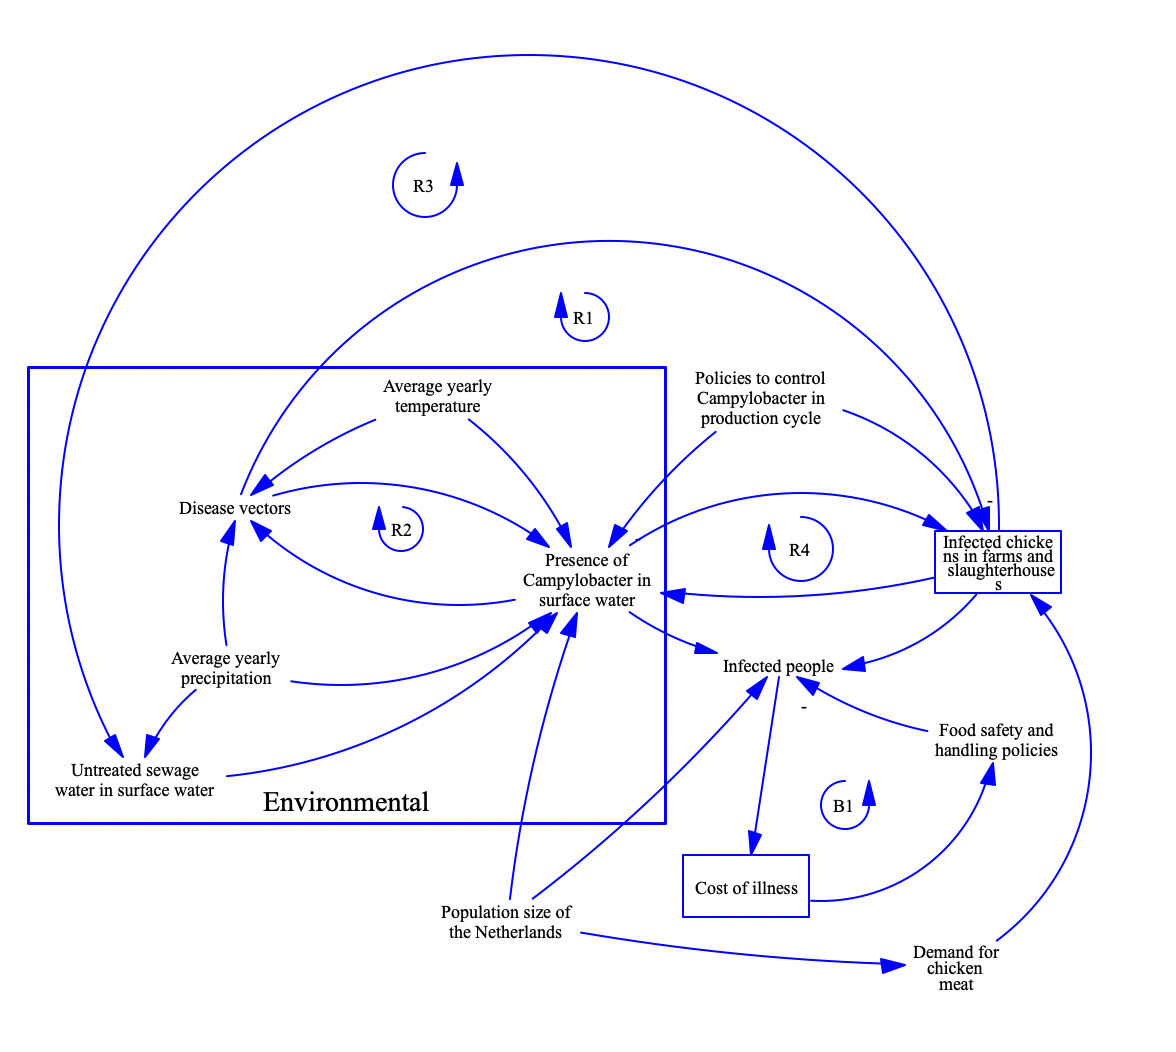
\includegraphics[width=0.5\textwidth]{images/dynamic_hypo.png}
\caption{The aggregated causal loop diagram for the dynamic hypothesis}
\end{figure}
 
\subsubsection*{Model Structure}
Although contamination is mainly concentrated on farms, the model will focus on farms and slaughterhouses collectively, rather than individual types of farms. This aligns better with decision-making regarding the general impacts of policy choices across the entire poultry industry in the Netherlands. This level of aggregation excludes most of the internal processes of slaughterhouses and broilers, as these are too detailed for this scope. Furthermore, this model will be tested against several climate scenarios which are based on the following assumptions: no new insect species are introduced into the system, despite their connection to climate change effects and spread of \textit{Campylobacter}, their influences were considered too detailed relative to the problem scoping. Lastly, the human population will be split into cohorts of children, working-age and seniors. Although cohorts based on age ranges would provide more accurate representation, the DALY used to calculate this cost of illness already incorporates age weightings \parencite{mangen_campylobacteriosis_2007}. 
\subsubsection*{Model Boundaries}

This model draws wider boundaries than Rommens' original model \parencite{rommens_infected_2020}. Here, the focus is on climate, population, and policy effects (both on production and consumption) and the subsequent economic impacts of these factors. As a result, some internal components of the model were simplified. Specifically, operational components related to transmissions occurring on individual farms, broilers, and slaughterhouses were aggregated into a single sub-model, allowing for more focus on environmental transmission pathways.

The sub-model of 'Infected Chickens' encompasses the majority of Rommens' original model \parencite{rommens_infected_2020}. Details of the structure and behaviour of this sub-model are detailed in the following sections.

\subsubsection*{Dynamic Hypothesis}
% is it okay to merge with conceptualisation?

\subsection{Explanation of model}
%3.	Explain model (also refer to Appendix A)
 %   a.	Describe sub-models
  %  b.	Explain most important assumptions
   
This analysis contains three main sub-models:

%Z: shorten the list in a couple of sentences? ¯\_(ツ)_/¯ 
\begin{itemize}
    \item Environmental %This sub-model focuses on environmental transmission routes and influences for \textit{Campylobacter}, particularly through surface waters and disease vectors (flies and birds other than poultry). According to recent reports by the RIVM, environmental transmission was the second most prevalent cause of \textit{Campylobacter} infections in the Netherlands in 2019. The sub-model also includes levers for climate influences on these transmission pathways.
    \item Infected chickens %This sub-model is based primarily on the work by Rommens. It is a simplified stock-flow model of her original work, designed to replicate key behaviours and interactions.
    \item Cost of illness %This sub-model tracks the impacts and probabilities of \textit{Campylobacter} infections leading to serious illness and fatality, including the relative cost of illness, to reflect economic effects of human \textit{Campylobacter} infections.

\end{itemize}

\subsubsection*{Environmental}
%LISETTEEEEEEEEEEEEEEEEEEEEEEEEEEEEEEEEEEEEEEEEEEEEEEEEEEEEEEEH
%IDENTIFY ARCHETYPES
%WHY IS THIS SO LONG AA

\begin{figure*}[!ht]
	\centering
	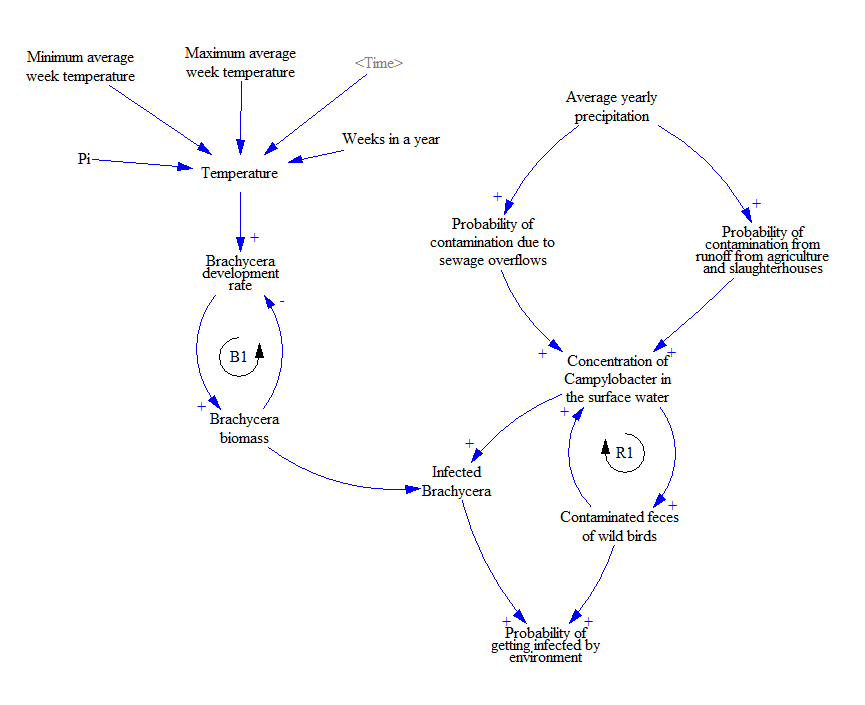
\includegraphics[width=0.5\textwidth]{images/environmental_submodel.png}
	\caption{The environmental sub-model}
	\label{fig:environmental_submodel}
\end{figure*}

\textit{Campylobacter} need humid surfaces to live, so surface water is recognised as a key player. Since animal faeces and runoff from agriculture and slaughterhouses enter nearby bodies of water, it is considered a good indicator for the amount of \textit{Campylobacter} present in the environment. Therefore, this has a big role in determining the chance of infection by biological disease vectors mentioned before. This can be seen in Figure~\ref{fig:environmental_submodel}. The main biological disease vectors have been determined to be flies and wild birds \parencite{mughini-gras_quantifying_2016}. Both vectors are considered to be major spreaders as they actively excrete \texitt{Campylobacter} on surfaces and human food \parencite{french_molecular_2009, hald_influxed_2008, berndtson_campylobacter_1996}.

It seems that the vector potential of flies is mainly determined by the \textit{Brachycera} suborder of the order \textit{Diptera}, and to be more specific by the \textit{Musca domestica}, which is more commonly known as the house fly \parencite{hald_influxed_2008}. We therefore opt to use the \textit{Musca domestica} as the model organism to represent the effects of the \textit{Diptera} insect order. \cite{skovgard_retention_2011} suggests that \textit{Musca domestica} are mainly short distance carriers of \textit{Campylobacter}. Therefore, the risk of transmission by \textit{Musca deomstica} is particularly high when the populations are greatest, which is during summer \parencite{royden_role_2016}. \cite{hald_use_2007} showed that preventing flies from entering houses in the summer of 2006 caused a significant drop in the prevalence of \textit{Campylobacter} at farms.

In Dutch and Luxembourgish waters, 37.7\% and 61.0\% of the \textit{Campylobacter} strains were attributed to poultry and wild birds respectively in a research by \cite{mughini-gras_quantifying_2016}. Since Luxembourg has a low poultry production, it is important to include this biological transmission vector in the sub-model.

Extreme temperatures are important selective agents during the separate stages of the \textit{Brachycera}. Climate change will cause the number of \textit{Brachycera} in the Netherlands to increase \parencite{goulson_predicting_2005}. It is expected this rise in numbers will be most evident in summer, but it is also expected in the winter according to \citeauthor{goulson_predicting_2005}. The climate driven population growth will also trigger migration, and therefore the dispersal \parencite{feder_locomotion_2010}, which will result in increased transmission of \textit{Campylobacter}. It is suspected that the total number of birds in the Netherlands is not affected by climate change, just their composition \parencite{mclean_reduced_2020, knudsen_challenging_2011}. Rainfall is not a driving factor in the total \textit{Brachycera} biomass \parencite{goulson_predicting_2005}.

Climate change is also linked to different precipitation patterns in the Netherlands. An increase in precipitation will result in increase of the Dutch sewer systems being overwhelmed and dumping the overflow in the environment, and will also result in an increase of contaminated runoff from agriculture and slaughterhouses \parencite{kwaad_summer_1991}.

An increase in Dutch population size is not expected to increase the \textit{Brachycera} biomass in the Netherlands \parencite{guenat_effects_2019}. Even though an increase in the population leads to more organic waste \parencite{garcia-garcia_framework_2015}, which does have the potential to increase the total number of flies \parencite{imai_population_1984, rozendaal_houseflies_1997}, this effect is possibly counterbalanced by the loss of natural habitat.

%Effect of climate change on runoff of Campylobacter and Cryptosporidium from land to surface water  This study shows that for the evaluated scenarios, climate change has little impact on concentrations of Campylobacter and Cryptosporidium transported from land to the surface waters.

% Seasonal effect on probability of infection through surface water?


\subsubsection*{Infected chickens}
% add sub-model diagram here
This sub-model (presented in Figure \ref{fig:transmission_submodel}) is a simplification of Rommens' 2020 model of dynamics of transmission in farms, broilers and slaughterhouses \parencite{rommens_infected_2020}. It is represented in our model as a stock-flow structure in which healthy chickens become infected chickens with \textit{Campylobacter} at the 'infection with \textit{Campylobacter}' rate. These infected chickens then become contaminated chicken meat when \textit{Campylobacter} positive chickens are slaughtered. Healthy chickens  contaminated chicken meat stock via '\textit{Campylobacter} negative chickens being slaughtered with cross-contamination. The contaminated chicken meat stock is reduced as contaminated chicken meat is consumed. The population of healthy chickens are also reduced by the flow variable '\textit{Campylobacter} negative chickens slaughtered without contamination'.

%David
\begin{figure}[h]
\centering
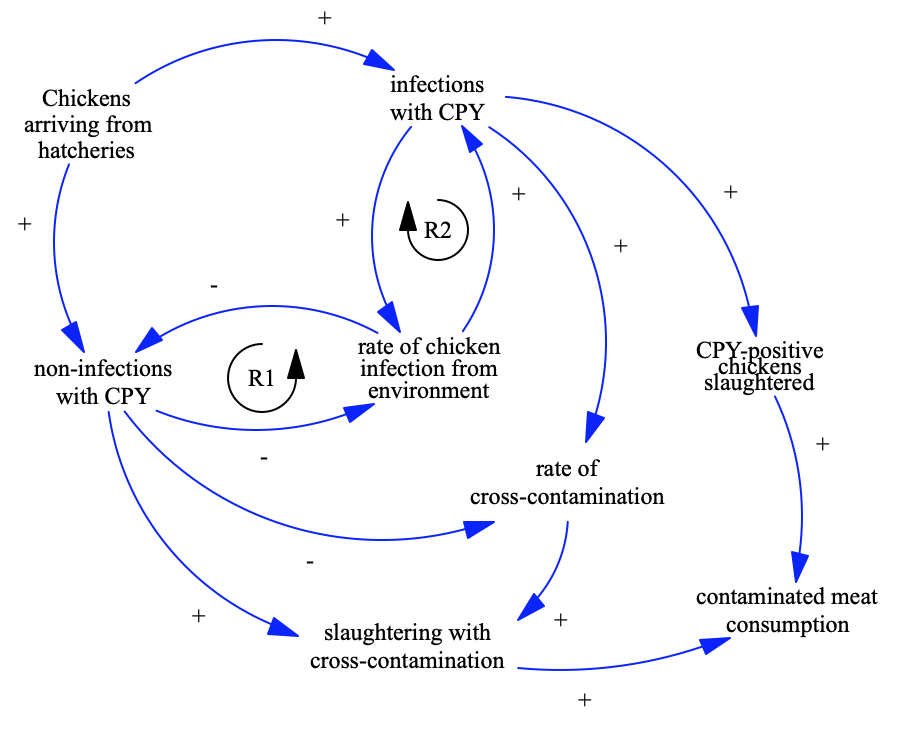
\includegraphics[width=1\textwidth]{images/Transmission submodel.png}
\caption{The conceptual chicken infection sub-model}
\label{fig:transmission_submodel}
\end{figure}

Other internal variables in this model included probabilities of infection, which are determined by environmental factors such as concentration of \textit{Campylobacter} in surface water, propagation of disease vectors, and climate effects, with the exact values for these rates detailed in Appendix~\ref{ch:model_documentation}.


\subsubsection*{Cost of illness}
%Emily
\begin{figure}[h]
\centering
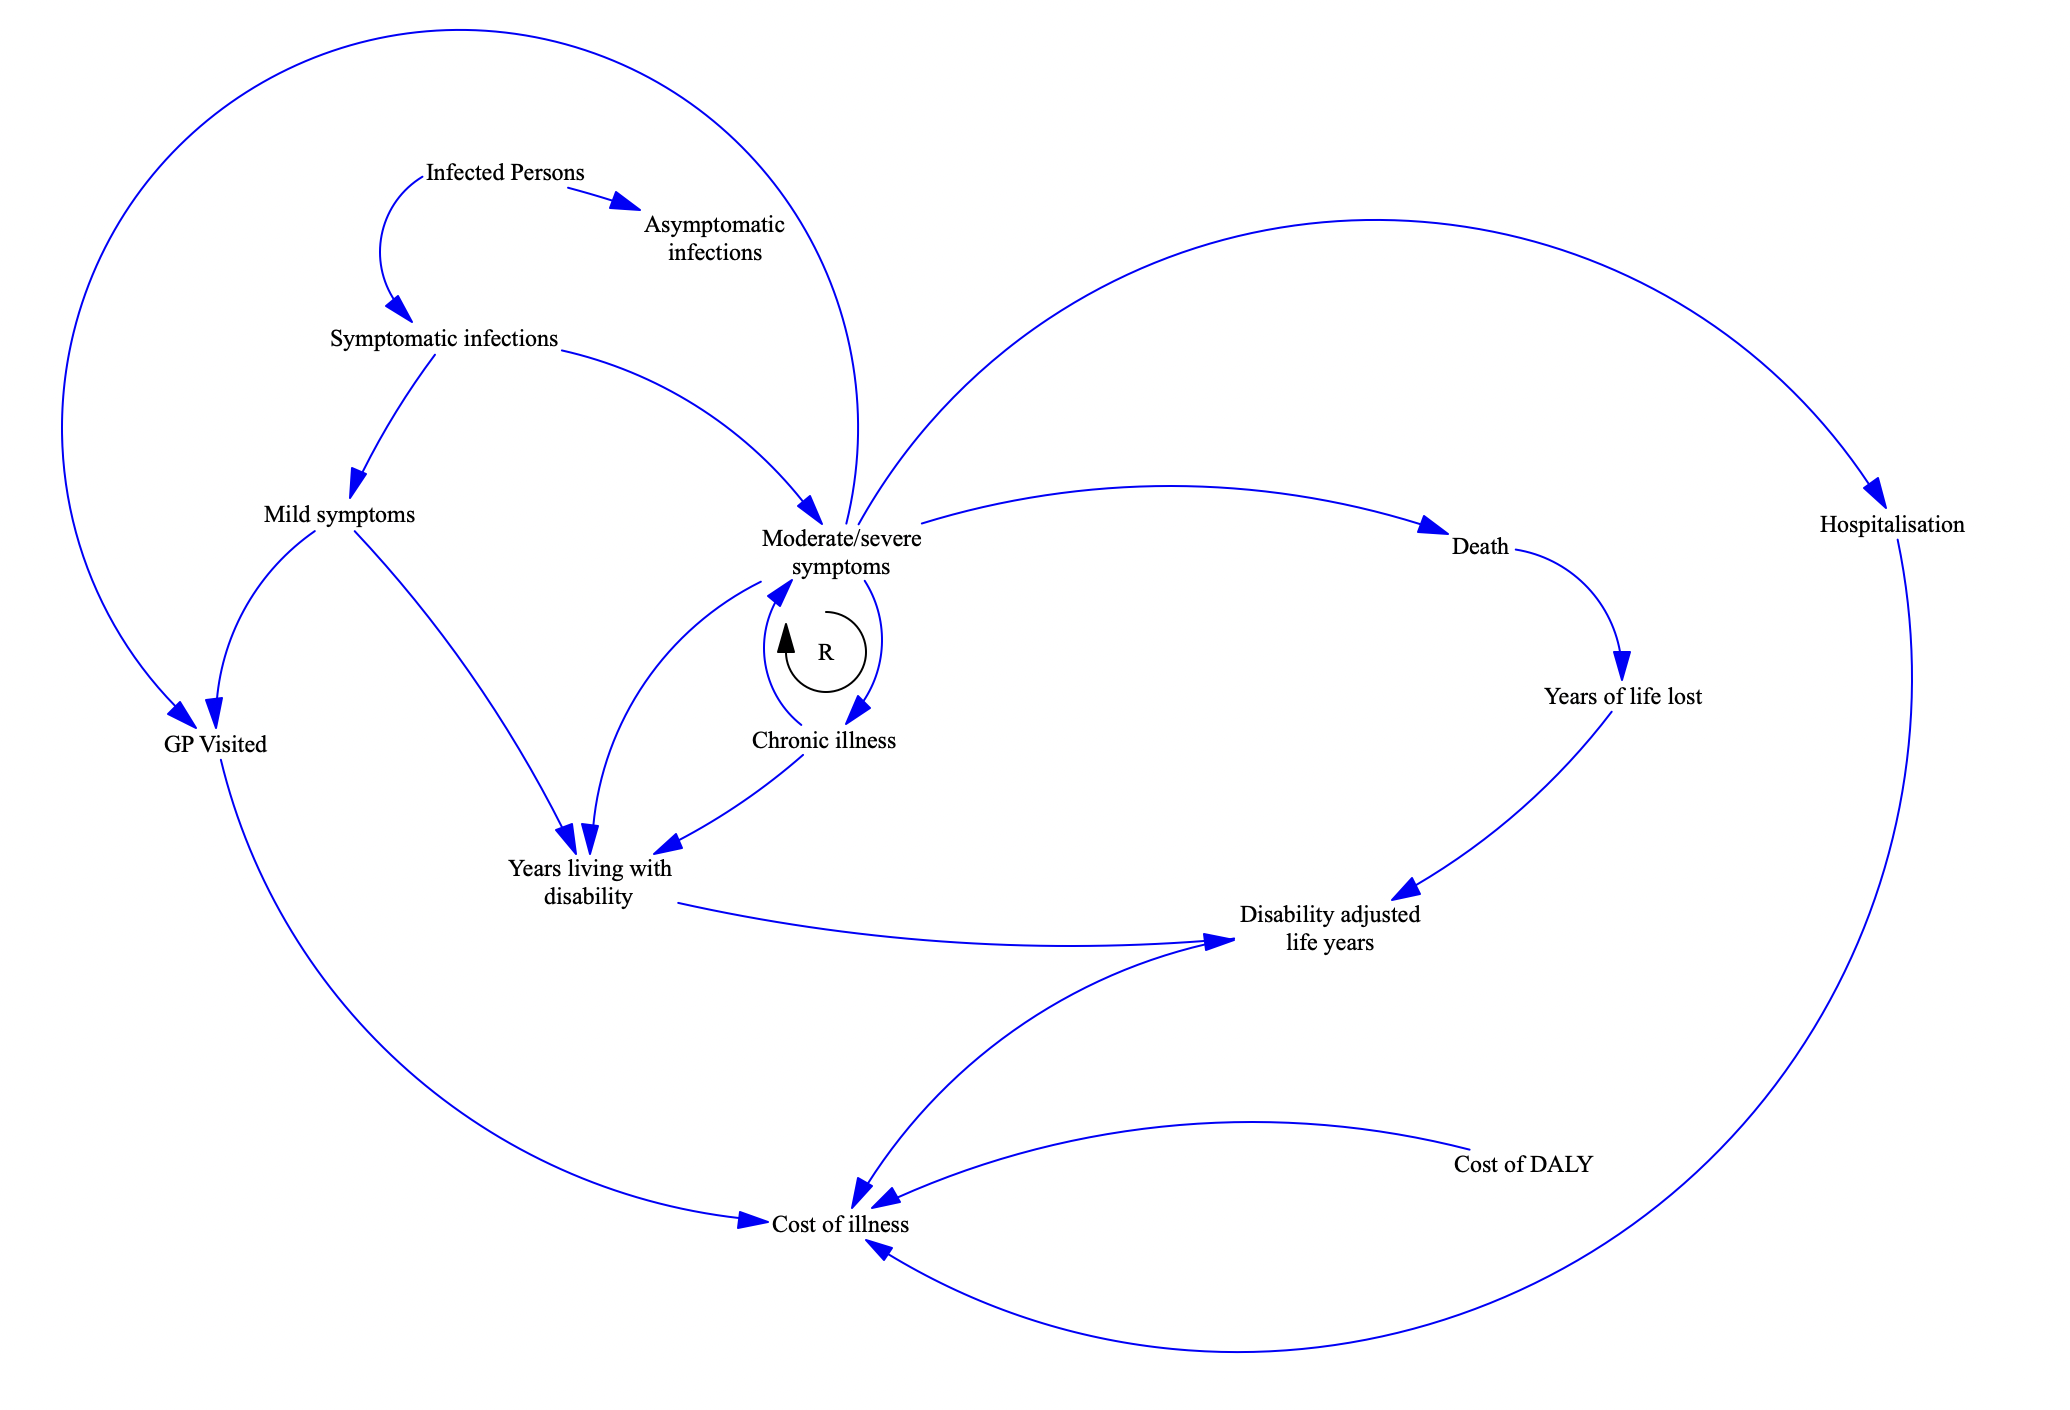
\includegraphics[width=0.5\textwidth]{images/COI_submodel.png}
\caption{The conceptual Cost of Illness sub-model}
\end{figure}
The cost of illness associated with \textit{Campylobacter} infections was modelled and calculated based primarily on a 2007 study by Mangen \parencite{mangen_campylobacteriosis_2007}. The Infected Persons stock is split off into symptomatic and asymptomatic infections. Symptomatic infections are assumed to all develop acute gastroenteritis, with a proportion of all cases either recovering, or subsequently developing chronic illnesses. Each of these outcomes contribute to key public health metrics of Disability Adjusted Life Years (DALYs) for these infections, and the Cost of Illness for all \textit{Campylobacter} infections. 

The causal structure adopted for this sub-model focuses on connecting variables based on available scientific data. Due to the underlying complexity of DALY and Cost of Illness metrics \parencite{jo_cost--illness_2014}, a top-down approach to applying these variables has been taken. As such, variables have been used for some elements that might otherwise have been modelled as stocks (e.g. DALYs and Cost of Illness). Additionally, this more simplistic approach is considered appropriate, as we are not concerned with the detailed dynamics of transmission and recovery (as might be done in an SIR model), but only with the ultimate KPIs of 'DALY' and 'Cost of Illness'.

\subsection{Key Assumptions}
%What were the key assumptions made in developing the model?
    %Take from validation spreadsheet
    %Include simplifications of real-world circumstances (e.g. acute campy coming before chronic conditions)

\subsection{Model Specification}
%What are the main mechanisms/variables/parameters in our model?

%What software was used for the modelling?
The system was modelled using VenSim PLE software developed by Ventana Systems Inc.
%Model Settings
    %Why was the integration method chosen?
The model uses Euler as the integration method. Euler was considered an attractive integration method for this model as it is suitable for integrating over non-linear and discontinuous functions (such as the pulse trains used to drain stocks), and it is a simple a direct method of integration. However, it does present some limitations in computational inefficiencies.
    %Why was the time step chosen?
TBC
    %Why was the time period chosen
The time period of \textcolor{red}{X} years was chosen to be able to show the effects of incremental changes in climate variability, whilst maintaining a small enough time step such that the transmission within chicken farms is realistic.
\subsection{Model Verification & Validation}
%4.	Validation
 %   a.	Use various tests to argue why model is fit for purpose
In this subsection we'll verify and validate the model. Verification will be done through a comparison with the conceptualisation of the model, as well as a unit verification and a time step verification. 

\subsubsection{Verification}


% From meeting with Jill:
%Verification requires three steps:
    %Check that the causal diagrams match the stock-flow diagrams, and add one line saying "this was checked'
    %Check that the units are consistent with the real world and add one line saying 'units were checked for material consistency'. -- DONE
Unit verification was performed by checking all variable units for ensure consistency with real-world equivalents. There was one anomalous variable in the model which could not be mapped to a physical value. This refers to the \textit{balancing constant} that feeds into the \textit{rate of fly development}. This was added under the assumption that temperature linearly correlates to fly populations, as documented by \citeauthor{blanckenhorn_adaptive_1998}, 1998. This factor allows conversion from the units of temperature (degrees) to fly development rate (MFly per week). This cannot be done without adding a go-between, which, in our case, is the balancing constant. 

Another noteworthy unit is that of the flow of \textit{Symptomatic infections}. The time unit used in the model is \textit{week}, to properly integrate seasonal changes in temperature across the year, months being to big and days too detailed. But for this same reason, DALY and COI are commonly reported per year. To deal with this, a PULSE TRAIN function was installed between stocks \textit{CPY Cases} and \textit{Acute GE Cases}. The PULSE TRAIN accumulates all \textit{Campylobacteriosis} cases over 52 weeks before transferring them to the cost of illness submodel. This can then be used as an input per year for the COI submodel. The units of the PULSE train remain in weeks when the time unit should be thought of as year, as happens after. 
    %Confirm that you've used the appropriate numerical technique/time step and add one line saying, 'behaviour of the model for the chosen time step and half that time step is consistent, this indicates that the appropriate time step and integration method has been used'

    
\subsubsection{Validation}    

%Validation requires three steps:
    %Show how the data matches or does not match historical data (explain why)
According to

    %Conduct an extreme values test to test the dynamic hypothesis and range of model applicability and provide comment to the reader on the boundaries of the model's effective use. Tell the reader the conditions under which the model behaves reliably
    %Generate the mode of behaviour/dynamic hypothesis - does it match, why or why not?
    
\subsection{Experimental setup}
%5.	Experimental setup
 %   a.	Introduce main uncertainties (potentially with table)
  %  b.	Explain scenario and policy logic
        %Parametric experiments - change parameters and observe behaviour (do multivariate for all, and univariate for one or two key variables)
        %Structural experiments - change a structure (e.g. add feedback) and observe behaviour 
   % c.	Number of runs, numerical integration method & time step, versions, etc.: all justified


\pagebreak

\section{Results}
\label{ch:results}
\iffalse
1.	Show and explain results without policies
2.	Show and explain consequences of scenarios for model behaviour
3.	Show and explain consequences of policies for each scenario (i.e., robustness) 
\fi
\subsection{Analysis Subsection}
\blindtext
\pagebreak

\section{Conclusion and Recommendations}
\label{ch:conclusion}
\subsection{1.	What was found?}
\textcolor{red}{Answer the research question from the intro}
\subsection{2.	What is the wider significance of what was found?}
\textcolor{red}{What are the policy recommendations from this analysis?}
\subsection{3.	Suggestions for further research}
\textcolor{red}{What are the limitations of the model (in terms of conceptualisation, specification, validation, and analysis?}
%Validation limitation = no validation with SME.
\begin{itemize}
    \item Expand the cost of illness and health impacts to look at health system capacity
    \item Explicitly model sub-components of DALYs for different population compositions to understand implications of aging population
    \item Model human infection from environment in more detail
    \item Reduce uncertainty by conducting household behavioural surveys before and after campylobacter infection
\end{itemize}

\pagebreak

%TC:ignore

\printbibliography


%\section{References}
%\bibliography{irrbibfile.bib}
\pagebreak

\pagenumbering{roman}

\appendix
\section{Model documentation}
\label{ch:model_documentation}
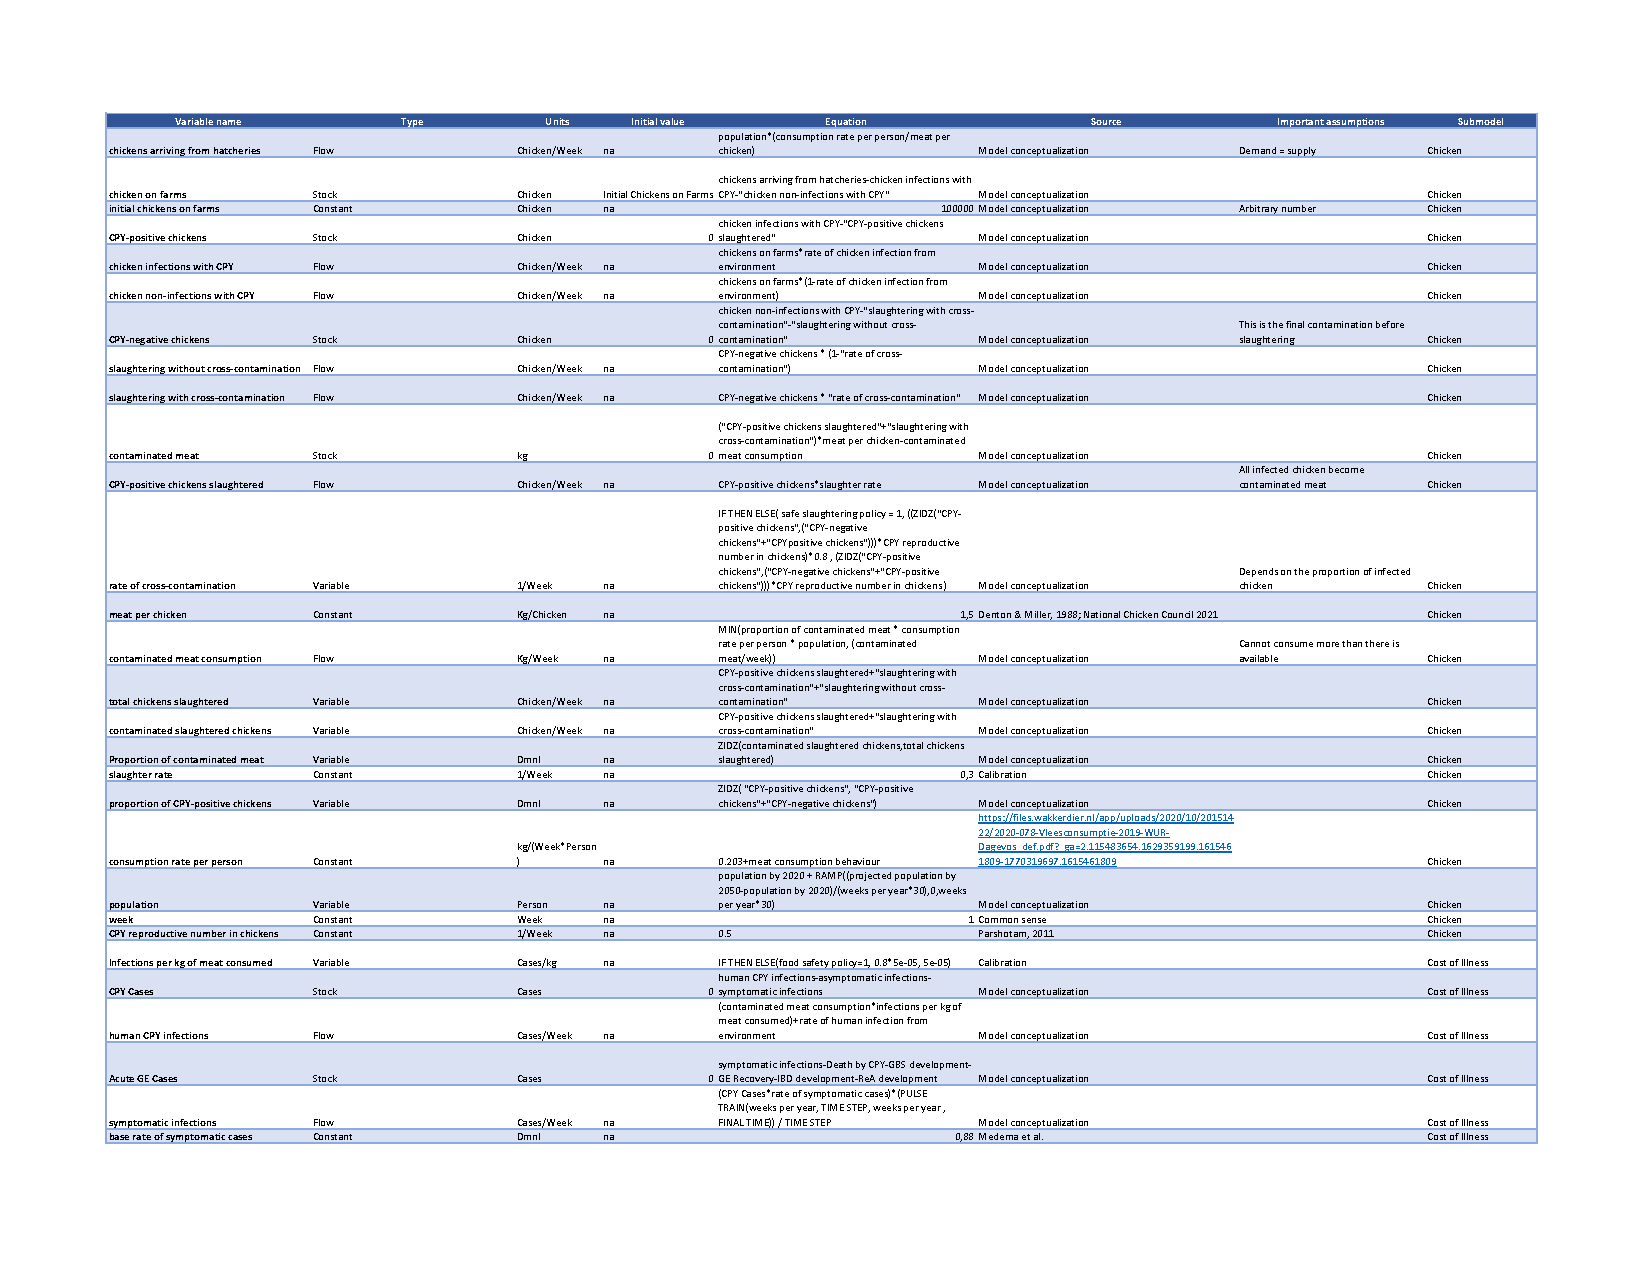
\includepdf[pages=-,landscape=true]{data/Stock Flow Variable Details.pdf}
%% Please add the following required packages to your document preamble:
% \usepackage{lscape}
% \usepackage{longtable}
% Note: It may be necessary to compile the document several times to get a multi-page table to line up properly
\begin{landscape}
\begin{longtable}[c]{m{10em}lllm{15em}lll}
\caption{}
\label{tab:my-table}\\
Variable name                                 & Type     & Units                    & Initial value             & Equation                                                                                                                                                                                                                                                                                 & Source                                                                                                                                                                                       & Important assumptions                                                                                                                                                                                                                 \\
\endfirsthead
%
\endhead
%
Chickens arriving from hatcheries             & Flow     & Chicken/week             &                           & Population * (consumption rate per person/meat per chicken)                                                                                                                                                                                                                              & Own interpretation                                                                                                                                                                           & Demand = supply                                                                                                                                                                                                                       \\
Chicken on farms                              & Stock    & Chicken                  & Initial Chickens on Farms & Chickens arriving from hatcheries - Chicken infections with CPY- Chicken non-infections with CPY'                                                                                                                                                                                        & Own interpretation                                                                                                                                                                           &                                                                                                                                                                                                                                       \\
Initial Chickens on farms                     & Constant & Chicken                  & na                        & 100000                                                                                                                                                                                                                                                                                   & Own interpretation                                                                                                                                                                           & Arbitrary number                                                                                                                                                                                                                      \\
CPY positive chickens                         & Stock    & Chicken                  & 0                         & Chicken infections with CPY - "CPY-positive chickens slaughtered"                                                                                                                                                                                                                        & Own interpretation                                                                                                                                                                           &                                                                                                                                                                                                                                       \\
Chicken infections with CPY                   & Flow     & Chicken/week             & na                        & Chicken on farms * rate of chicken infection from environment                                                                                                                                                                                                                            & Own interpretation                                                                                                                                                                           &                                                                                                                                                                                                                                       \\
Chicken non-infections with CPY               & Flow     & Chicken/week             & na                        & Chickens on farms * (1-rate of chicken infection from environment)                                                                                                                                                                                                                       & Own interpretation                                                                                                                                                                           &                                                                                                                                                                                                                                       \\
CPY negative chickens                         & Stock    & Chicken                  & 0                         & Chicken non-infections with CPY' - 'slaughtering with cross-comtamination' - 'slaughtering without cross-contamination'                                                                                                                                                                  & Own interpretation                                                                                                                                                                           & This is the final contamination before slaughtering                                                                                                                                                                                   \\
Slaughtering without cross-contamination      & Flow     & Chicken/week             &                           & CPY-negative Chickens' * (1- 'rate of cross-contamination')                                                                                                                                                                                                                              & Own interpretation                                                                                                                                                                           &                                                                                                                                                                                                                                       \\
Slaughtering with cross-contamination         & Flow     & Chicken/week             &                           & CPY-negative Chickens' *'rate of cross-contamination'                                                                                                                                                                                                                                    & Own interpretation                                                                                                                                                                           &                                                                                                                                                                                                                                       \\
Contaminated meat                             & Stock    & kg                       & 0                         & ('CPY positive Chickens slaughtered' + 'slaughtering with cross-contamination") * Meat per chicken  - Meat Consumption                                                                                                                                                                   & Own interpretation                                                                                                                                                                           &                                                                                                                                                                                                                                       \\
CPY-positive chickens slaughtered             & Flow     & Chicken/week             & na                        & CPY-positive chickens*slaughter rate                                                                                                                                                                                                                                                     & Own interpretation                                                                                                                                                                           &                                                                                                                                                                                                                                       \\
Rate of cross-contamination                   & Variable & 1/Week                   & na                        & ZIDZ("CPY-positive chickens",("CPY-negative chickens"+"CPY-positive chickens"))*0.5                                                                                                                                                                                                      & Own interpretation                                                                                                                                                                           & Depends on the proportion of infected chicken                                                                                                                                                                                         \\
Meat per chicken                              & Constant & Kg/chicken               & na                        & 1,5                                                                                                                                                                                                                                                                                      &                                                                                                                                                                                              &                                                                                                                                                                                                                                       \\
Contaminated Meat consumption                 & Flow     & Kg/week                  & na                        & MIN(proportion of contaminated meat * consumption rate per person * Population, (Contaminated Meat/week))                                                                                                                                                                                &                                                                                                                                                                                              & Cannot consume more than there is available                                                                                                                                                                                           \\
Total Chickens slaughtered                    & Variable & Chicken/week             & na                        & CPY-positive Chickens slaughtered' + 'slaughtering with cross-contamination' + 'slaughtering without cross-contamination')                                                                                                                                                               &                                                                                                                                                                                              &                                                                                                                                                                                                                                       \\
Contaminated slaughtered Chickens             & Variable & Chicken/week             & na                        & slaughtering with cross-contaminsation' + 'CPY-positive Chickens slaughtered'                                                                                                                                                                                                            &                                                                                                                                                                                              &                                                                                                                                                                                                                                       \\
Proportion of contaminated meat               & Variable & Dmnl                     & na                        & ZIDZ('Contaminated slaughtered Chickens, Total Chickens slaughtered)                                                                                                                                                                                                                     &                                                                                                                                                                                              &                                                                                                                                                                                                                                       \\
consumption rate per person                   & Constant & kg/(week*person)         & na                        & 0,203+meat consumption behaviour                                                                                                                                                                                                                                                         & https://files.wakkerdier.nl/app/uploads/2020/10/20151422/2020-078-Vleesconsumptie-2019-WUR-Dagevos\_def.pdf?\_ga=2.115483654.1629359199.1615461809-1770319697.1615461809                     &                                                                                                                                                                                                                                       \\
Population                                    & Variable & person                   & na                        & population by 2020 + RAMP((project population by 2050 - population by 2020) / (weeks per year * 30) , 0 , weeks per year * 30 )                                                                                                                                                          & PLACEHOLDER                                                                                                                                                                                  &                                                                                                                                                                                                                                       \\
Slaughter rate                                & Constant & 1/week                   & na                        & 0,3                                                                                                                                                                                                                                                                                      & PLACEHOLDER                                                                                                                                                                                  &                                                                                                                                                                                                                                       \\
Infections per kg of meat consumed            & Constant & Cases/kg                 & na                        & 5e0.5                                                                                                                                                                                                                                                                                    & PLACEHOLDER                                                                                                                                                                                  &                                                                                                                                                                                                                                       \\
CPY Cases                                     & Stock    & Cases                    & 0                         & Human CPY infections - asymptomatic infections - symptomatic infections                                                                                                                                                                                                                  & Own interpretation                                                                                                                                                                           &                                                                                                                                                                                                                                       \\
Human CPY infections                          & Flow     & Cases/week               &                           & (Contaminated meat consumption * infections per kg of meat consumed ) + rate of human infection from environment                                                                                                                                                                         &                                                                                                                                                                                              &                                                                                                                                                                                                                                       \\
Acute GE cases                                & Stock    & Cases                    &                           & Symptomatic infections-Death by CPY-GBS development-GE Recovery-IBD development-ReA development                                                                                                                                                                                          &                                                                                                                                                                                              &                                                                                                                                                                                                                                       \\
Symptomatic infections                        & Flow     & Cases/week               &                           & (CPY Cases * Rate of symptomatic cases)*(PULSE TRAIN(weeks per year, TIMESTEP, weeks per year, FINAL TIME))/TIMESTEP                                                                                                                                                                     &                                                                                                                                                                                              &                                                                                                                                                                                                                                       \\
rate of symptomatic cases                     & Constant & Dmnl                     & na                        & 0,88                                                                                                                                                                                                                                                                                     & Medema et al.                                                                                                                                                                                &                                                                                                                                                                                                                                       \\
Asymptomatic infections                       & Flow     & Cases/week               & na                        & (CPY Cases * (1-Rate of symptomatic cases))*(PULSE TRAIN(weeks per year, TIMESTEP, weeks per year, FINAL TIME))/TIMESTEP                                                                                                                                                                 &                                                                                                                                                                                              &                                                                                                                                                                                                                                       \\
GE Recovery                                   & Flow     & Cases/week               & na                        & recovery rate*Acute GE cases                                                                                                                                                                                                                                                             &                                                                                                                                                                                              &                                                                                                                                                                                                                                       \\
recovery rate                                 & Constant & 1/Week                   & na                        & 0,98125                                                                                                                                                                                                                                                                                  &                                                                                                                                                                                              &                                                                                                                                                                                                                                       \\
ReA Cases                                     & Stock    & Cases                    & 0                         & ReA development                                                                                                                                                                                                                                                                          &                                                                                                                                                                                              &                                                                                                                                                                                                                                       \\
GBS Cases                                     & Stock    & Cases                    & 0                         & GBS development                                                                                                                                                                                                                                                                          &                                                                                                                                                                                              &                                                                                                                                                                                                                                       \\
IBD Cases                                     & Stock    & Cases                    & 0                         & IBD development                                                                                                                                                                                                                                                                          &                                                                                                                                                                                              &                                                                                                                                                                                                                                       \\
Death by CPY                                  & Flow     & Cases/week               & na                        & Acute GE Cases*death rate                                                                                                                                                                                                                                                                & Own interpretation                                                                                                                                                                           & Disease burden/cost of illness associated with deaths accounted for within DALY metric. This flow used to empty the cases stock                                                                                                       \\
ReA development                               & Flow     & Cases/week               & na                        & Acute GE Cases*ReA Rate                                                                                                                                                                                                                                                                  & Own interpretation                                                                                                                                                                           & Development of chronic disease assumed to all occur subsequent to acute cases. In reality, some campylobacter infections do connect directly to incidence of chronic disease.                                                         \\
GBS development                               & Flow     & Cases/week               & na                        & Acute GE Cases*GBS Rate                                                                                                                                                                                                                                                                  & Own interpretation                                                                                                                                                                           &                                                                                                                                                                                                                                       \\
IBD development                               & Flow     & Cases/Week               & na                        & Acute GE Cases*IBD development                                                                                                                                                                                                                                                           & Own interpretation                                                                                                                                                                           &                                                                                                                                                                                                                                       \\
ReA Rate                                      & Constant & 1/Week                   &                           & 0,0175                                                                                                                                                                                                                                                                                   & Mangen et al.                                                                                                                                                                                &                                                                                                                                                                                                                                       \\
GBS Rate                                      & Constant & 1/Week                   & na                        & 0,00075                                                                                                                                                                                                                                                                                  & Mangen et al.                                                                                                                                                                                &                                                                                                                                                                                                                                       \\
IBD Rate                                      & Constant & 1/Week                   & na                        & 0,000125                                                                                                                                                                                                                                                                                 & Mangen et al.                                                                                                                                                                                & Rate doubled to account for increase in diagnosis of IBD over past 2 decades: https://www.cdc.gov/ibd/data-statistics.htm\#:$\sim$:text=Inflammatory\%20Bowel\%20Disease\%20Prevalence\%20(IBD,\%25\%20or\%202\%20million\%20adults). \\
death rate                                    & Constant & 1/Week                   & na                        & 0,000375                                                                                                                                                                                                                                                                                 & Mangen et al.                                                                                                                                                                                & Assumed that death only caused by acute symptoms, death from chronic cases largely contained within DALYs.                                                                                                                            \\
weeks per year                                & Constant & Week                     & na                        & 52                                                                                                                                                                                                                                                                                       & This is how time works.                                                                                                                                                                      &                                                                                                                                                                                                                                       \\
Fly population                                & Stock    & Mfly                     & initial fly population    & Fly development - Fly death                                                                                                                                                                                                                                                              & Own interpretation                                                                                                                                                                           &                                                                                                                                                                                                                                       \\
Fly deaths                                    & Flow     & Mfly/week                & na                        & DELAY1I(fly development, fly lifetime, fly population/fly lifetime)                                                                                                                                                                                                                      &                                                                                                                                                                                              &                                                                                                                                                                                                                                       \\
Fly development                               & Flow     & Mfly/week                & na                        & fly development rate                                                                                                                                                                                                                                                                     &                                                                                                                                                                                              &                                                                                                                                                                                                                                       \\
Initial fly population                        & Constant & Mfly                     & na                        & 0,1                                                                                                                                                                                                                                                                                      &                                                                                                                                                                                              &                                                                                                                                                                                                                                       \\
Fly lifetime                                  & Constant & Week                     & na                        & 4                                                                                                                                                                                                                                                                                        & THERE IS A SOURCE                                                                                                                                                                            &                                                                                                                                                                                                                                       \\
Balancing constant                            & Constant & MFly/(degree*Week)       & na                        & 1                                                                                                                                                                                                                                                                                        & Blanckenhorn, W. U. (1997). Effects of temperature on growth, development and diapause in the yellow dung fly - against all the rules? Oecologia, 111(3), 318–324. doi:10.1007/s004420050241 & This constant helps units balance for the empirical formula                                                                                                                                                                           \\
Balancing constant 2                          & Constant & 1/Week                   &                           & 1                                                                                                                                                                                                                                                                                        &                                                                                                                                                                                              &                                                                                                                                                                                                                                       \\
Fly development rate                          & Variable & Dmnl                     & na                        & (-0.0091 + 0.0024 * MAX ( Temperature, 4)) * Balancing constant                                                                                                                                                                                                                          & Blanckenhorn, W. U. (1997). Effects of temperature on growth, development and diapause in the yellow dung fly - against all the rules? Oecologia, 111(3), 318–324. doi:10.1007/s004420050241 &                                                                                                                                                                                                                                       \\
Temperature                                   & Variable & degree                   & na                        & \begin{tabular}[c]{@{}l@{}}((-1)*(SIN(2*pi*(Time+start of year offset)/weeks per year))*((maximum average weekly temperature-minimum average weekly temperature\\    )/2)+((maximum average weekly temperature+minimum average weekly temperature)/2))+temperature increase\end{tabular} & Own interpretation                                                                                                                                                                           &                                                                                                                                                                                                                                       \\
Minimum average weekly temperature            & Variable & degree                   & na                        & -4                                                                                                                                                                                                                                                                                       & KNMI                                                                                                                                                                                         &                                                                                                                                                                                                                                       \\
Maximum average weekly temperature            & Variable & degree                   & na                        & 23                                                                                                                                                                                                                                                                                       & KNMI                                                                                                                                                                                         &                                                                                                                                                                                                                                       \\
Pi                                            & Variable & Dmnl                     & na                        & ARCCOS(-1)                                                                                                                                                                                                                                                                               & Archimedes of Syracuse                                                                                                                                                                       &                                                                                                                                                                                                                                       \\
Start of year offset                          & Variable & Week                     & na                        & 8                                                                                                                                                                                                                                                                                        & it's 2 months                                                                                                                                                                                &                                                                                                                                                                                                                                       \\
proportion of infectious flies                & Variable & Dmnl                     & na                        & 0.35 + 0.5 * "proportion of CPY positive chickens"                                                                                                                                                                                                                                       & PLACEHOLDER                                                                                                                                                                                  &                                                                                                                                                                                                                                       \\
infectious flies                              & Variable & Mfly                     & na                        & fly population*proportion of infectious flies                                                                                                                                                                                                                                            & Own interpretation                                                                                                                                                                           &                                                                                                                                                                                                                                       \\
Rate of chicken infection from environment    & Variable & 1/week                   & na                        & 0.1+(infectious flies*rate of chicken exposure to infectious flies)                                                                                                                                                                                                                      & Own interpretation                                                                                                                                                                           &                                                                                                                                                                                                                                       \\
Rate of human infection from environment      & Variable & 1/(Mfly*Person)          & na                        & infectious flies*rate of human exposure to infectious flies*population + (infection risk from birds * population)                                                                                                                                                                        & Own interpretation                                                                                                                                                                           &                                                                                                                                                                                                                                       \\
Rate of chicken exposure to infectious flies  & Variable & 1/(Mfly*Week)            & na                        & 2                                                                                                                                                                                                                                                                                        & PLACEHOLDER                                                                                                                                                                                  &                                                                                                                                                                                                                                       \\
Rate of human exposure to infectious flies    & Constant & Cases/(Mfly*Week*person) & na                        & 0.001                                                                                                                                                                                                                                                                                    & frate                                                                                                                                                                                        &                                                                                                                                                                                                                                       \\
DALY                                          & Variable & DALY                     &                           & (DALYs per GE Case * Acute GE Cases) + (DALYs per ReA Case * ReA Cases) + (DALYs per GBS Case * GBS Cases) + (DALYs per IBD Case * IBD Case)                                                                                                                                             &                                                                                                                                                                                              &                                                                                                                                                                                                                                       \\
Cost of Illness                               & Variable & Euro                     &                           & (COI per GE Case * Acute GE Cases) + (COI per ReA Case * ReA Cases) + (COI per GBS Case * GBD Cases) + (COI per IBD Case * IBS Case)                                                                                                                                                     &                                                                                                                                                                                              &                                                                                                                                                                                                                                       \\
DALYs per GE Case                             & Constant & DALY/Case                &                           & 0,008                                                                                                                                                                                                                                                                                    & Mangen et al.                                                                                                                                                                                & All undiscounted DALYs                                                                                                                                                                                                                \\
DALYs per ReA Case                            & Constant & DALY/Case                &                           & 0,09                                                                                                                                                                                                                                                                                     & Mangen et al.                                                                                                                                                                                & All undiscounted DALYs                                                                                                                                                                                                                \\
DALYs per GBS Case                            & Constant & DALY/Case                &                           & 5                                                                                                                                                                                                                                                                                        & Mangen et al.                                                                                                                                                                                & All undiscounted DALYs                                                                                                                                                                                                                \\
DALYs per IBD Case                            & Constant & DALY/Case                &                           & 11,6                                                                                                                                                                                                                                                                                     & Mangen et al.                                                                                                                                                                                & All undiscounted DALYs                                                                                                                                                                                                                \\
COI per GE Case                               & Constant & Euros/Case               &                           & 190                                                                                                                                                                                                                                                                                      & Mangen et al.                                                                                                                                                                                &                                                                                                                                                                                                                                       \\
COI per ReA Case                              & Constant & Euros/Case               &                           & 20                                                                                                                                                                                                                                                                                       & Mangen et al.                                                                                                                                                                                &                                                                                                                                                                                                                                       \\
COI per GBS Case                              & Constant & Euros/Case               &                           & 85000                                                                                                                                                                                                                                                                                    & Mangen et al.                                                                                                                                                                                &                                                                                                                                                                                                                                       \\
COI per IBD Case                              & Constant & Euros/Case               &                           & 173000                                                                                                                                                                                                                                                                                   & Mangen et al.                                                                                                                                                                                &                                                                                                                                                                                                                                       \\
week                                          & Constant & Week                     &                           & 1                                                                                                                                                                                                                                                                                        & Common sense                                                                                                                                                                                 &                                                                                                                                                                                                                                       \\
average temperature increase                  & Variable & degree                   &                           & RAMP(temperature increase by 2050/(weeks per year*30),0,weeks per year*30)                                                                                                                                                                                                               & Own interpretation                                                                                                                                                                           &                                                                                                                                                                                                                                       \\
temperature increase                          & Variable & degree                   &                           & IF THEN ELSE(temperature switch = 0,0,(IF THEN ELSE(temperature switch = 2,(-1)*(SIN(2*pi*(Time+start of year offset)/weeks per year)*0.8*average temperature increase)+average temperature increase,average temperature increase)))                                                     & Bresser et al, 2006                                                                                                                                                                          &                                                                                                                                                                                                                                       \\
temperature increase by 2050                  & Constant & degree                   &                           & 1,5                                                                                                                                                                                                                                                                                      & KNMI 14' klimaatscenario's voor Nederland                                                                                                                                                    &                                                                                                                                                                                                                                       \\
proportion of CPY-positive chickens           & Variable & Dmnl                     &                           & ZIDZ("CPY-positive chickens", "CPY,positive chickens" + "CPY-negative chickens")                                                                                                                                                                                                         &                                                                                                                                                                                              &                                                                                                                                                                                                                                       \\
Recovered GE                                  & Stock    & Cases                    &                           & GE Recovery                                                                                                                                                                                                                                                                              &                                                                                                                                                                                              &                                                                                                                                                                                                                                       \\
Consumer food preparation behaviour lever     & Lever    & Dmnl                     &                           & IF THEN ELSE(  (CPY Cases/Population) \textgreater consumer food preparation behaviour threshold , 1 , 0 )                                                                                                                                                                               &                                                                                                                                                                                              &                                                                                                                                                                                                                                       \\
Consumer food preparation behaviour threshold & Constant & Euro                     & na                        & 0.0038                                                                                                                                                                                                                                                                                   & SOURCE?                                                                                                                                                                                      &                                                                                                                                                                                                                                       \\
population by 2020                            & Constant & Person                   & na                        & 1,73E+07                                                                                                                                                                                                                                                                                 &                                                                                                                                                                                              &                                                                                                                                                                                                                                       \\
population by 2050                            & Constant & Person                   &                           & 2.16E+0.7                                                                                                                                                                                                                                                                                &                                                                                                                                                                                              &                                                                                                                                                                                                                                       \\
Infection risk from birds                     & Constant & Cases/(Person*Week)      &                           & 2.5E-0.5                                                                                                                                                                                                                                                                                 &                                                                                                                                                                                              &                                                                                                                                                                                                                                       \\
                                              &          &                          &                           &                                                                                                                                                                                                                                                                                          &                                                                                                                                                                                              &                                                                                                                                                                                                                                       \\
Exposure control policies                     &          &                          &                           &                                                                                                                                                                                                                                                                                          &                                                                                                                                                                                              & Question for Irene Friday - can we start stocks at 0 (for chickens), allow model to build up and show once the balanced behaviour achieved?                                                                                           \\
Fly population control policy                 &          &                          &                           &                                                                                                                                                                                                                                                                                          &                                                                                                                                                                                              &                                                                                                                                                                                                                                       \\
Food safety and handling policy               & Switch   & Dmnl                     & 1                         & IF THEN ELSE( Cost of Illness \textgreater 100000000 , 1 , 0 )                                                                                                                                                                                                                           &                                                                                                                                                                                              &                                                                                                                                                                                                                                       \\
Meat consumption behaviour                    & Variable & kg/week                  &                           &                                                                                                                                                                                                                                                                                          &                                                                                                                                                                                              &                                                                                                                                                                                                                                       \\
Food preparation policy                       &          &                          &                           &                                                                                                                                                                                                                                                                                          &                                                                                                                                                                                              &                                                                                                                                                                                                                                       \\
temperature switch                            & Constant & Dmnl                     &                           & 2                                                                                                                                                                                                                                                                                        & \begin{tabular}[c]{@{}l@{}}0 - No change\\    1 - Linear change\\    2 - Faster summer warming than winter warming\end{tabular}                                                              &                                                                                                                                                                                                                                       \\
                                              &          &                          &                           &                                                                                                                                                                                                                                                                                          &                                                                                                                                                                                              &                                                                                                                                                                                                                                       \\
                                              &          &                          &                           &                                                                                                                                                                                                                                                                                          &                                                                                                                                                                                              &                                                                                                                                                                                                                                       \\
                                              &          &                          &                           &                                                                                                                                                                                                                                                                                          &                                                                                                                                                                                              &                                                                                                                                                                                                                                      
\end{longtable}
\end{landscape}
\section{Validation}
\label{ch:validation} 
\textcite{vlaanderen_staat_2019} estimated there were around 71.000 cases of Campylobacteriosis in the Netherlands in 2018, 67.000 in 2017 and 79.000 in 2016. We plotted the amount of cases produced by our model against the average of these three values. The results can be seen in Figure~\ref{fig:val_human_cases}. It can be seen that a lot more people are symptomatic than the average of the estimated values. About a million people are infected within our model, which is 2 order of magnitudes more than the average.
{\color{pink}GIVE REASON}

\textcite{nepluvi_rapportage_2019} monstered broiler chickens weekly in 2018, and found $41,9$-$58.1\%$ of broilerchickens were tested positive for \textit{Campylobacter}. This concerns chickens from slaughterhouses. As can be seen in Figure~\ref{fig:val_chickens}, our base model has similar values for each year.

In the Netherlands the (unsanitary) preparation and/or consumption of chicken were attributed to $20$-$30\%$ of infections in 2018. However, around $50$-$80\%$ of cases can be attributed to \textit{Campylobacter} strains associated with poultry \parencite{cuperus_surveillance_2020, nepluvi_rapportage_2019}. Therefore, it is safe to assume that there are multiple transmission routes. We assume the biggest transmission routes can be found in the environment. In the base model, around 5.70\% of the infections stem from the preparation and/or consumption of chicken. This can be seen in Figure~\ref{fig:val_sources}. It may be the case that the environment plays a bigger role than we previously assumed, after all, it is easier to trace back the cause to undercooked meat than to a wild bird.

We also validated our DALYs and Cost of Illness against the datapoints from \parencite{mangen_campylobacteriosis_2007}. Note that these values are from 2007. As can be seen in Figure~\ref{fig:val_dalys} our model determines higher DALYs than given in the literature. This may indicate that there are more chronic diseases that can be traced back to \textit{Campylobacter} than is currently happening in the real world. Perhaps the specialists are overlooking the bacterium as a cause, or they are simply unable to pinpoint the cause.

In Figure~\ref{fig:val_coi} it can be seen that the Cost of Illness calculated by the model is lower than \citeauthor{mangen_campylobacteriosis_2007}'s values. This is probably due to the fact that we only look at 3 chronic conditions and the acute conditions. 

It is estimated there are around 17 million species of \textit{Diptera} per person \parencite{gorman_trillions_2017}. We are only interested in \textit{Musca domestica}. It is unknown what their numbers are in the Netherlands, and we are unable to estimate. However, it has been guessed that the population of Houseflies will increase by 244\% by 2080 \parencite{mcalister_secret_2017}. In The amount of flies in our model after 1 year is 20.000 of which 7.700 are infectious (TIME STEP = 0.0625). This is probably not a proper reflection of the real world, but one can assume that it is only 7.700 flies that have directly caused a disease in humans and/or chickens.

The model also includes an Infection risk from birds (2.5e-05). There are about 1.3 million birds in the Netherlands \parencite{noauthor_miljoenen_2019}. There was no literature on the risk from birds, so we assumed a somewhat safe value. We doubt \textit{Campylobacter} will ever be exterminated due to the presence of these environmental factors, even if we are somehow able to keep our farms, slaughterhouses and stores free from \textit{Campylobacter}.

%to include: meat consumption

\begin{figure*}[!h]
    \centering
    \begin{minipage}{0.45\textwidth}
        \centering
        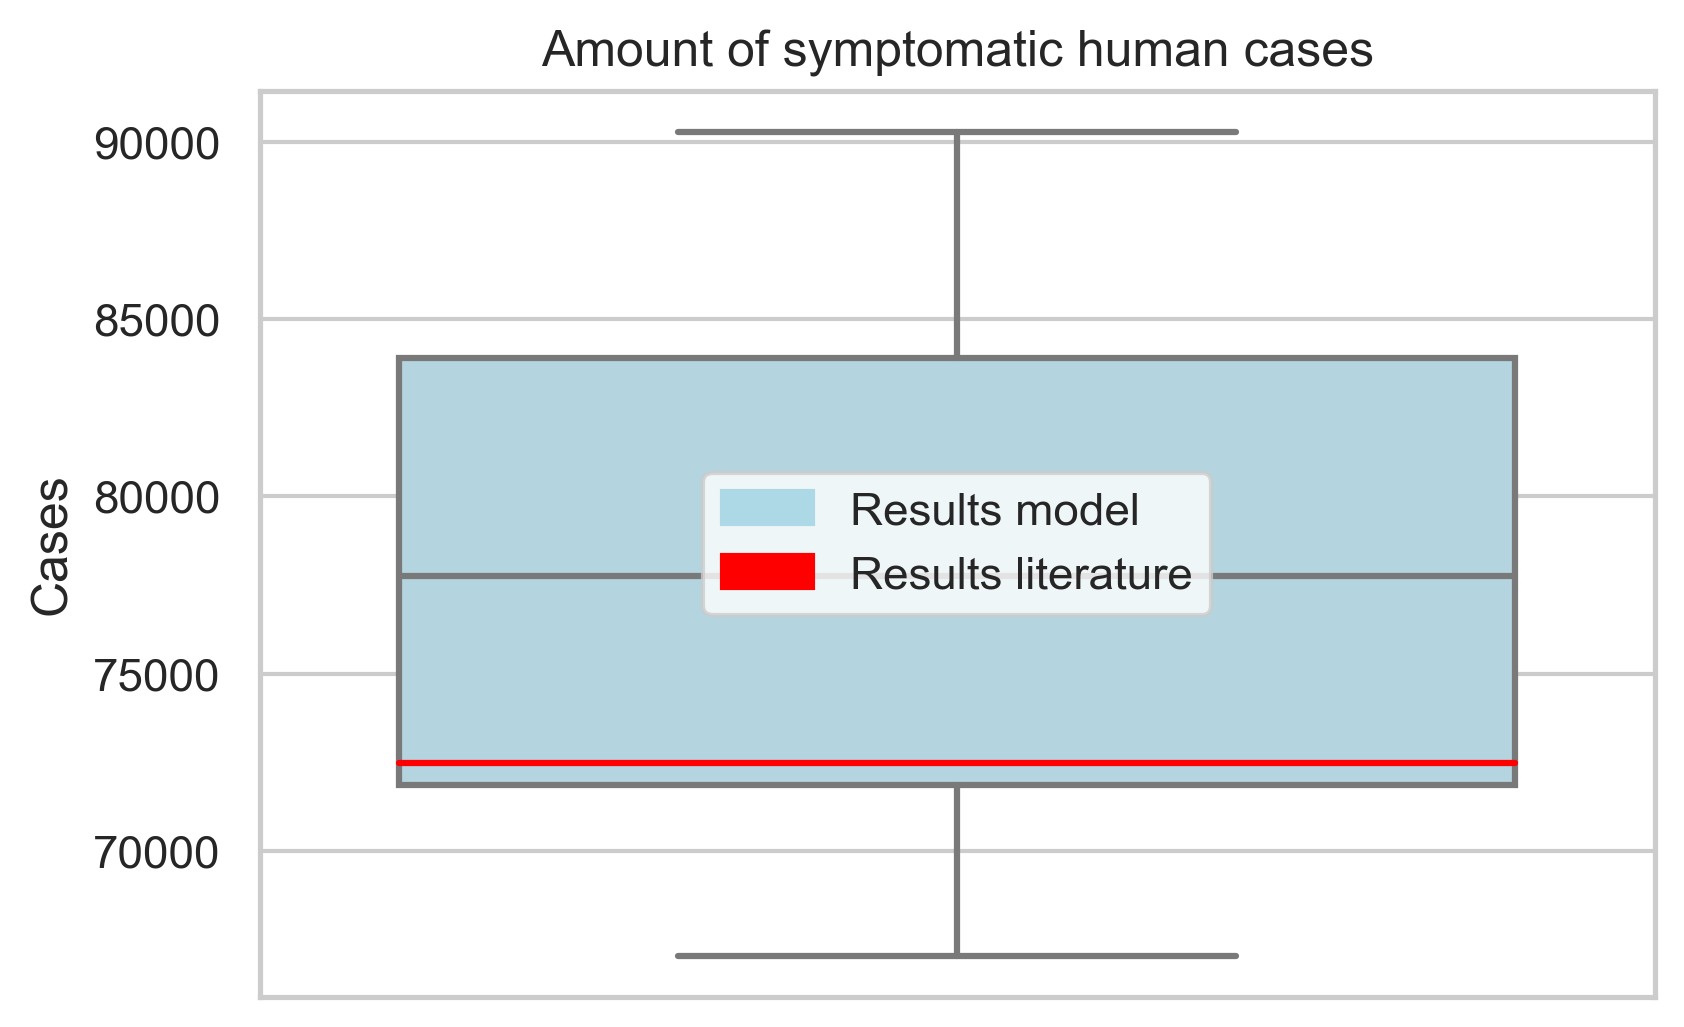
\includegraphics[width=0.9\textwidth]{notebooks/human_cases2.png} % first figure itself
        \caption{Validation of human cases}
        \label{fig:val_human_cases}
    \end{minipage}\hfill
    \begin{minipage}{0.45\textwidth}
        \centering
        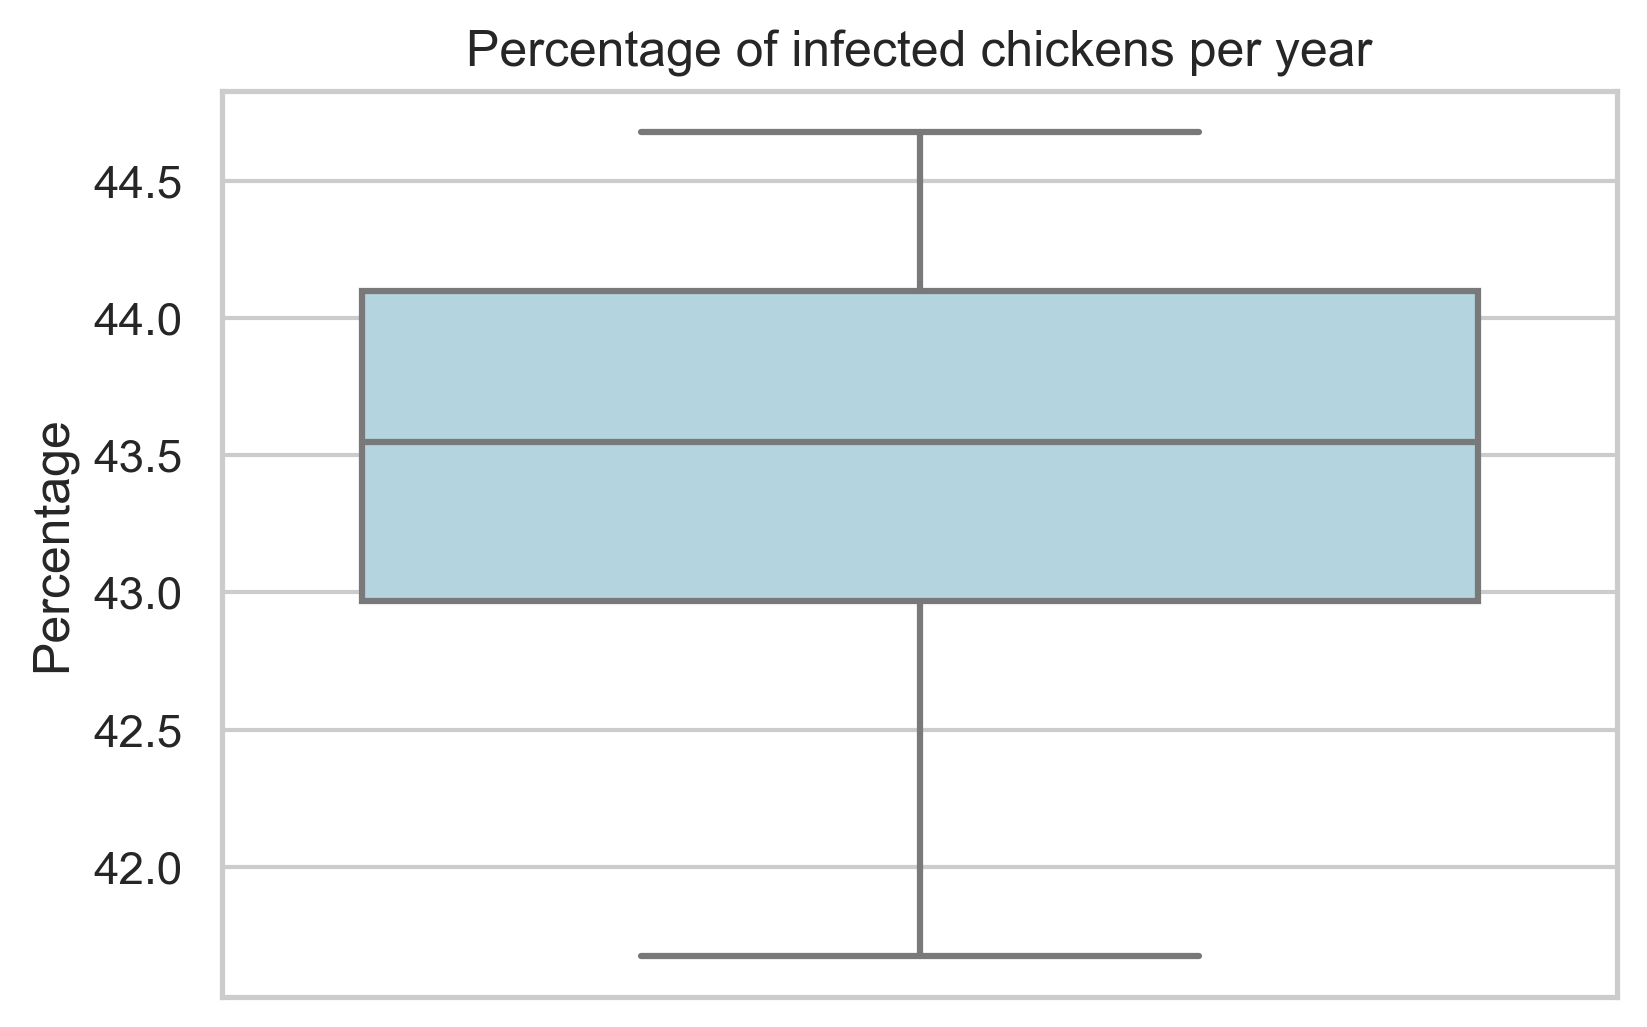
\includegraphics[width=0.9\textwidth]{notebooks/chickens2.png} % second figure itself
        \caption{Validation of proportion infected chickens}
	    \label{fig:val_chickens}
    \end{minipage}
\end{figure*}

\begin{figure*}[!h]
	\centering
	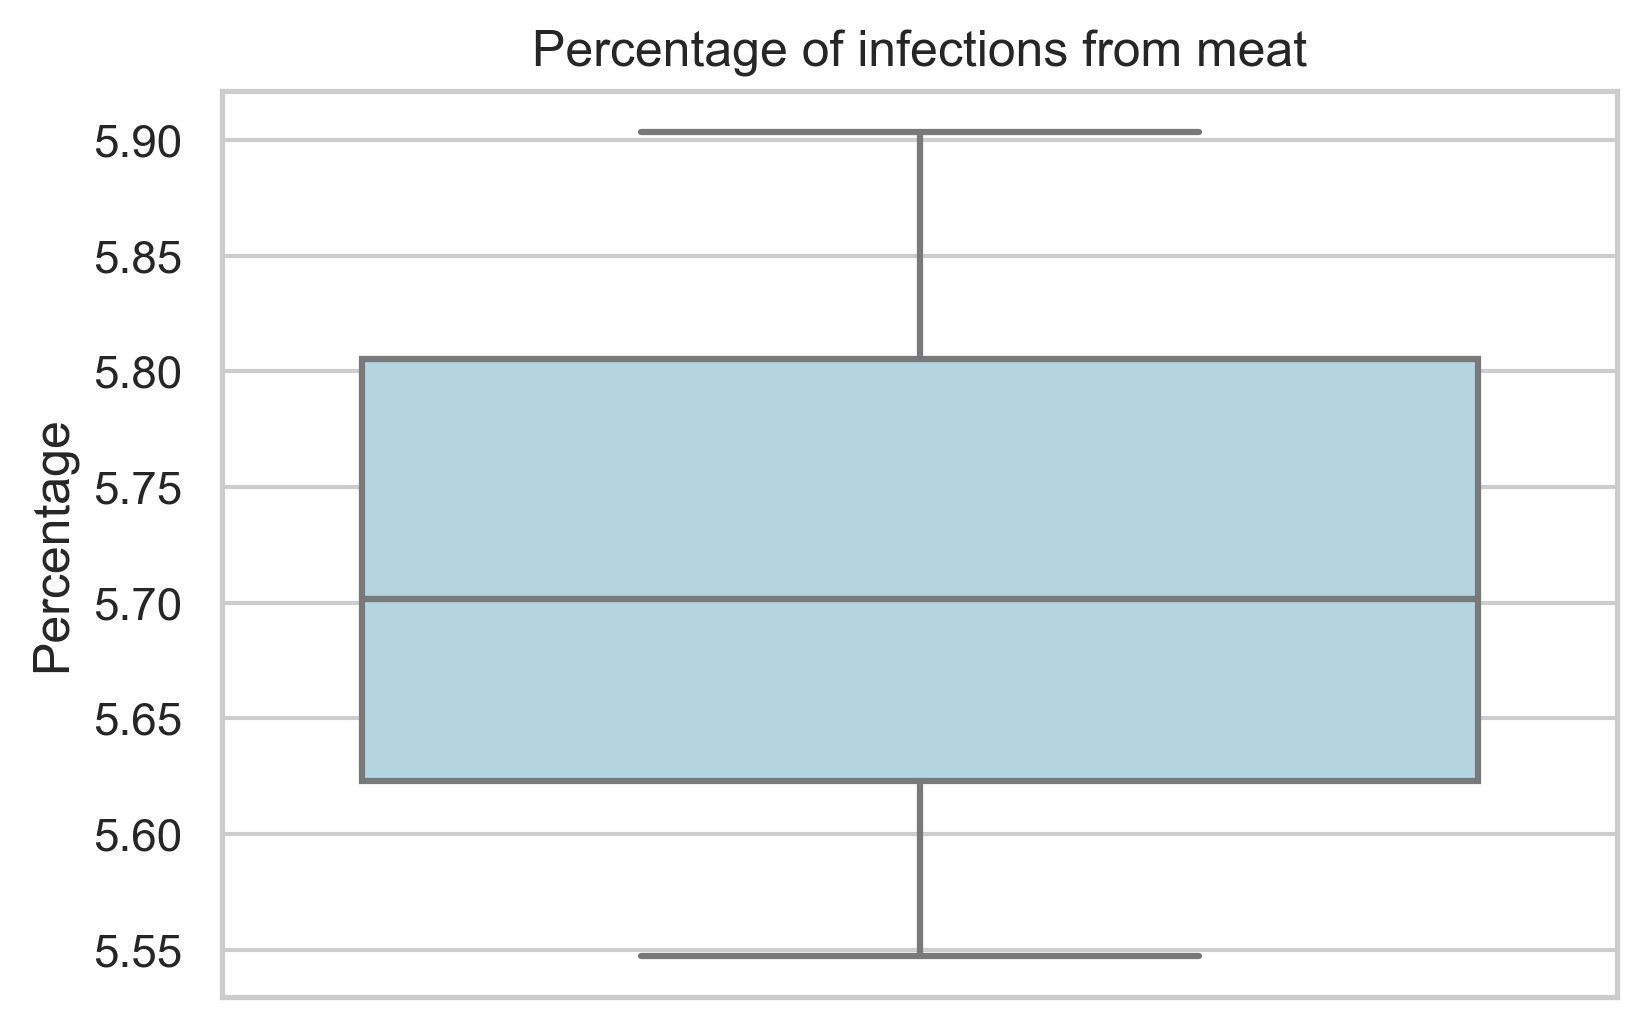
\includegraphics[width=0.5\textwidth]{notebooks/source2.png}
	\caption{Validation of sources of Campylobacteriosis}
	\label{fig:val_sources}
\end{figure*}

\begin{figure*}[!h]
    \centering
    \begin{minipage}{0.45\textwidth}
        \centering
        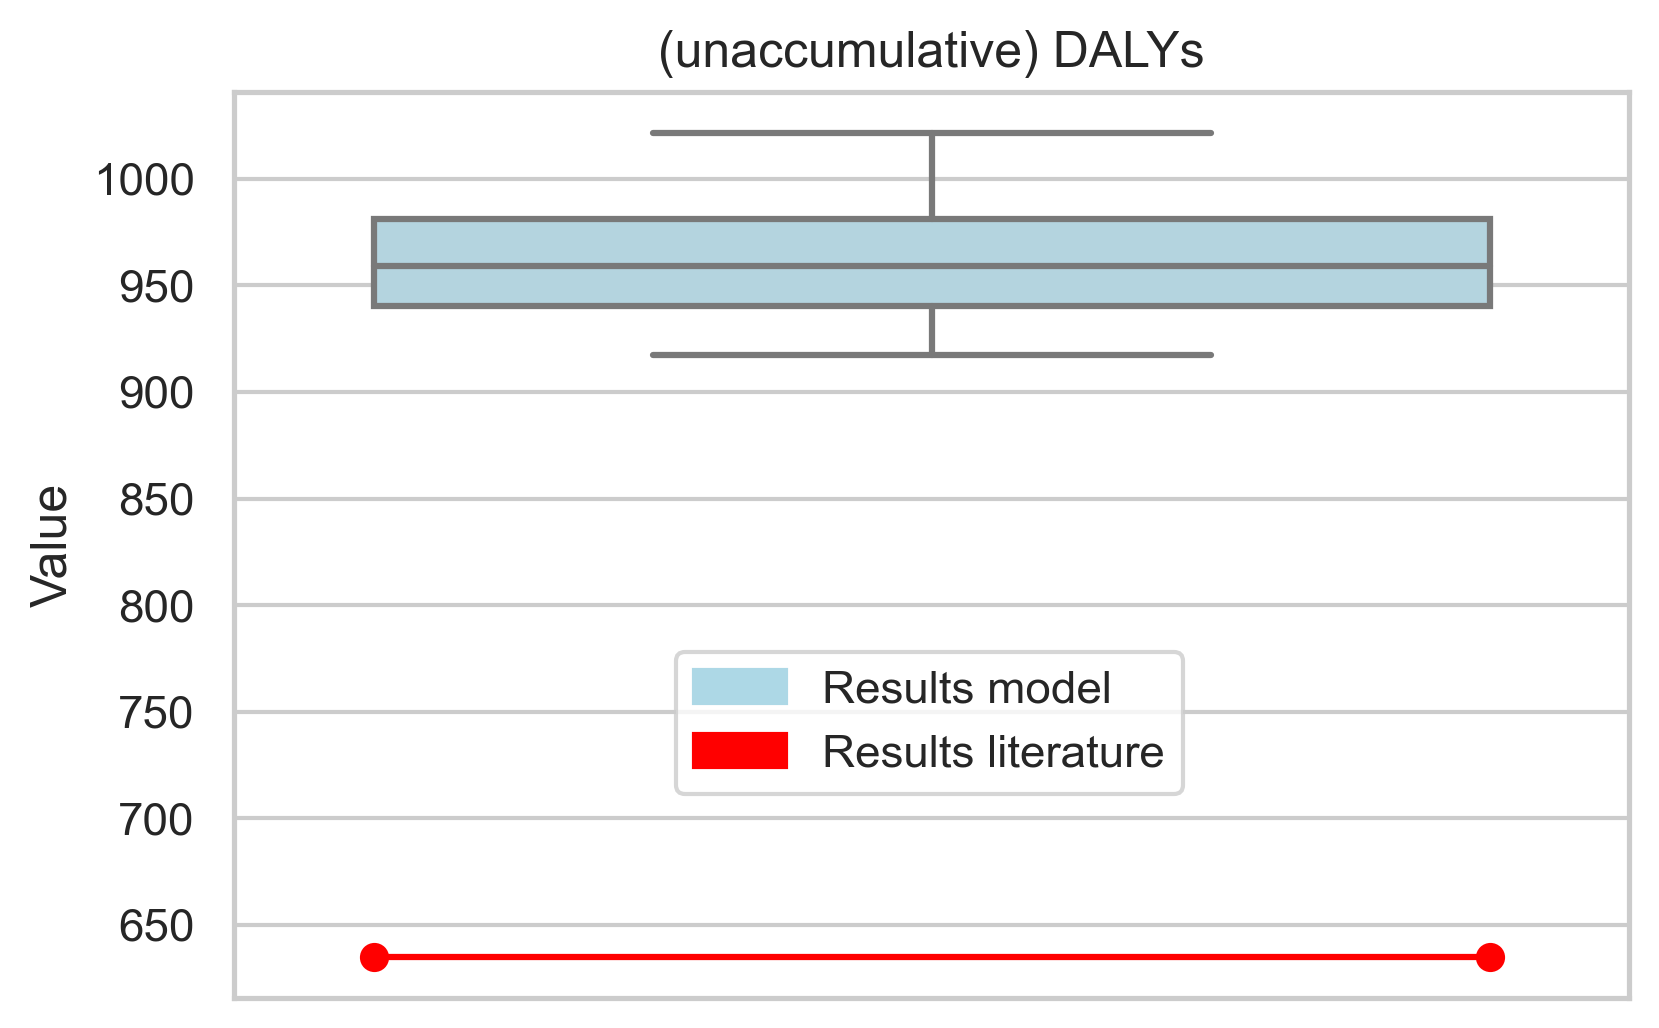
\includegraphics[width=0.9\textwidth]{notebooks/dalys2.png} % first figure itself
        \caption{Validation of DALYs}
	    \label{fig:val_dalys}
    \end{minipage}\hfill
    \begin{minipage}{0.45\textwidth}
        \centering
        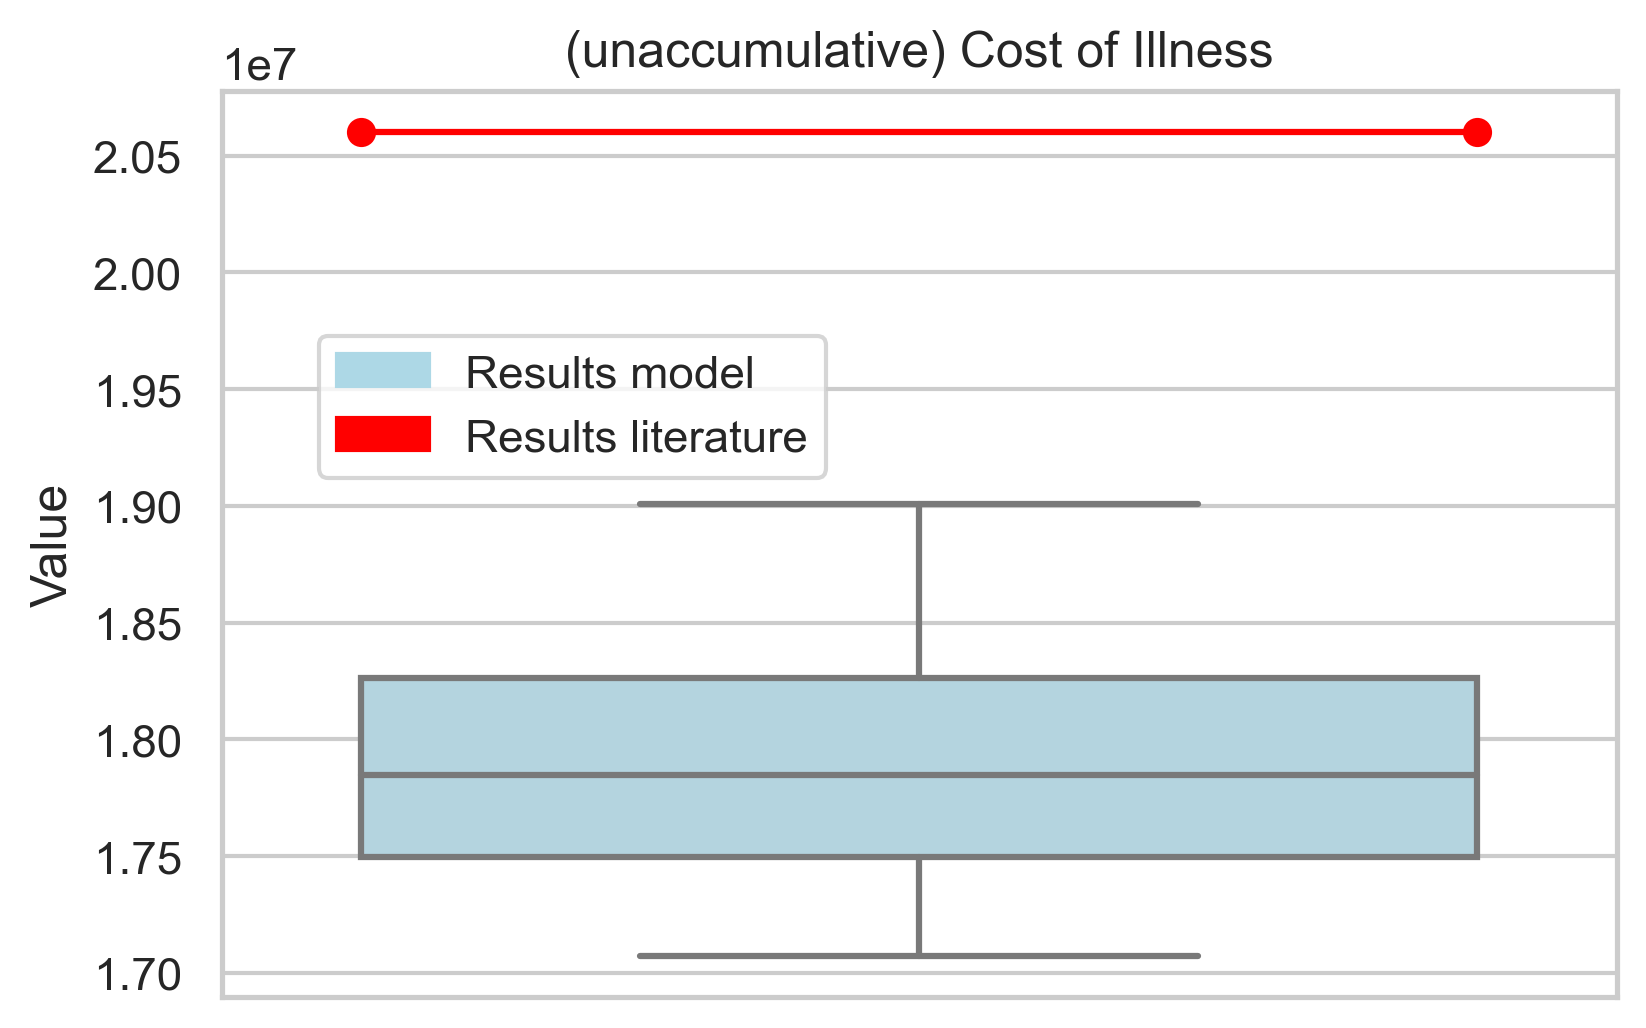
\includegraphics[width=0.9\textwidth]{notebooks/coi2.png} % second figure itself
        \caption{Validation of Cost of Illness}
	    \label{fig:val_coi}
    \end{minipage}
\end{figure*}
\clearpage
\section{Details on policies and experiments}
\label{ch:det_policies} 
%TC:ignore

To answer our research question, experiments were set up around the three components in the research question: climate, population and public health. 

The structural and parametric uncertainties resulted in five policies that will be tested. These policies were designed based on reality and are capable of providing a view of the policies' cost effectiveness and robustness. These policies will be discussed in Subsection \ref{s:environmentalfactors} to \ref{s:foodbehaviour}. 

We elaborate on the scenarios used to test these policies in Subsection~\ref{ch: detexp}.

%Policies in environment
\subsection{Environmental factors and policies to control disease vectors}
\label{s:environmentalfactors}
Two policies were implemented with regards to environmental factors and the biological disease vectors. Both are triggered by temperature, as this is the main driver of the population growth of flies, as explained in Section~\ref{fig:environmental_submodel}.

\subsubsection{Exposure control policy}
This policy decreases human exposure to infected flies: on the season when the disease vector is more prevalent, public campaigns will urge the population to keep organic waste properly closed and use fly nets \parencite{hald_use_2007}. Similar measures are used to prevent the spread of disease carrying mosquitoes in tropical countries \parencite{govella_why_2012}. %I know this for a fact because tropical country, but we might want to add a source.

The closed-loop policy is triggered by the temperature. If the temperature is above 20\degree c, the policy goes in effect. This temperature is based on the findings by \cite{schou_temperature_2013}. It assumes an immediate reduce of 20\% on the rate of human exposure to infectious flies. It was also assumed there would be an information delay of 2 weeks from the onset of the policy to full implementation.

\subsubsection{Fly population control policy}
When a certain threshold of fly population is reached, the government can initiate extermination campaigns to limit the spread of diseases. This can be generalised, or localised only around farms.

Likewise to the Exposure control policy, this policy is activated by temperature. Once the temperature gets above 20\degree c, the policy goes into effect. This immediately reduces the fly population to 80\%. We assume the effect is immediate, as this policy is not dependent on people's behaviour: the government can instantiate these immediately.

\iffalse
\begin{itemize}
    \item Public campaigns to prevent human exposure to infected flies: on the season when the disease vector is more prevalent, urge the population to keep organic waste properly closed and use fly nets \parencite{hald_use_2007}. Similar measures are used to prevent the reproduction of disease carrying mosquitoes in tropical countries. %I know this for a fact because tropical country, but we might want to add a source.
    \item Pest control measures: when a certain threshold of fly population is reached, the government can initiate extermination campaigns to limit the spread of diseases. This can be generalised, or localised only around farms.
%install pest control measures, including variables such as: intensity of extermination / frequency
%install threshold fly population value that activates pest control. The aim is to counteract effects of population growth to infected flies and infection rates.
%Note: could we connect fly population or proportion of infected flies to exposure rate??
\end{itemize}
\fi


\subsection{Food safety behaviours and policies}
\label{s:foodbehaviour}
With regards to food safety behaviours and policies, we looked at two insertion points in the chicken production cycle: the hygiene of the slaughtering process and the way food is handled from the slaughterhouse to the consumer. Lastly, we also looked at the effectiveness of a policy that addresses consumer behaviour by discouraging meat consumption.

\subsubsection{Safe slaughtering Policy}
%Policies on chicken farms
This policy would try to address and improve the level of hygiene of slaughterhouse process and equipment, which has been identified to be a major transmission. Specifically this policy would for instance require slaughterhouse equipment to be cleaned using water that is frequently changed to prevent cross-contamination. This can also be enhanced by the use of UV radiation to aid in the decontamination process without altering the sensory quality of the meat \parencite{isohanni_use_2009}.

In the model this was implemented by adding a switch variable that turned on if the COI of the the previous year exceed a certain amount, in this case set to \euro 15 million, to reduce the \textit{rate of cross-contamination cross-contamination} by 20\%. It is of note that the switch activates the modifier immediately upon reaching the threshold, thus operating under the assumption that there is no delay in policy trigger and its implementation. In reality it will take time to adopt the policy, but effects are negligible at the 30-year time scale.

\subsubsection{Food safety and handling policy}
This policy deals with the way chicken products are handled by both consumers and actors in the production cycle of chicken meat. If the quality of the routines in the preparation, transport and storage of chicken  products is increased, there will be a reduction in foodborne illnesses such as campylobacteriosis~\parencite{shane_campylobacter_2000}.

When the Cost of Illness of past year has exceeded the threshold value of \euro 15 million, this policy is triggered. So, effectively, there is a delay of 1 year. There is 20\% less chance to get infected by the consumption of meat once this policy is in effect.

\subsubsection{Consumption behaviour policy}
With this policy, instead of attempting to disrupt \textit{Campylobacter} transmission routes among chickens and other animals, it circumvents the central issue and addresses meat consumption. This would include any measure that would dissuade or restrict the consumption of chicken meat throughout the population, e.g. campaigns, meat tax, etc.

The policy also operates with a threshold-activated switch. The threshold was set higher to \euro 22 million compared to the safe slaughtering policy, as it is seen as "last resort", because it seems unlikely that meat bans would be complied to, nor be implemented in the first place, as meat consumption in the Netherlands is still on the rise.

%Policies in COI 
\iffalse
\begin{itemize}
    \item Food safety and handling: Policy connecting cost of illness to proportion of contaminated chicken
    \item Behavioural link from DALYs to either infections per kg consumed OR kg of chicken meat consumed. There is a structural uncertainty related to how consumer behaviour might change. Will individuals reduce their chicken consumption or will they be more careful in food handling?
\end{itemize}
\fi

\iffalse
\subsection*{Note on policy implementation}
Policies were implemented using switches, connecting directly to the variable it is meant to address. This is not realistic as policies will exhibit side effects. To more accurately integrate policies into the system,  a group modelling approach is recommended, including relevant stakeholders such as farmers, policy experts, and public health practitioners \parencite{vennix_group_1999}.
\fi

\iffalse
\subsubsection{Effect of policies on the base model}
A policy regarding slaughtering was modelled into the base model, which will be tested under the same scenarios as the base model. The food safety and handling policy, also dubbed the Safe Slaughtering policy, goes into effect when Cost of Illness reaches a certain threshold, set at a 100 million euros. This policy means that the rate of cross-contamination drops by 20\%.  

\begin{figure}[h!]
    \centering
    \begin{minipage}{0.45\textwidth}
        \centering
        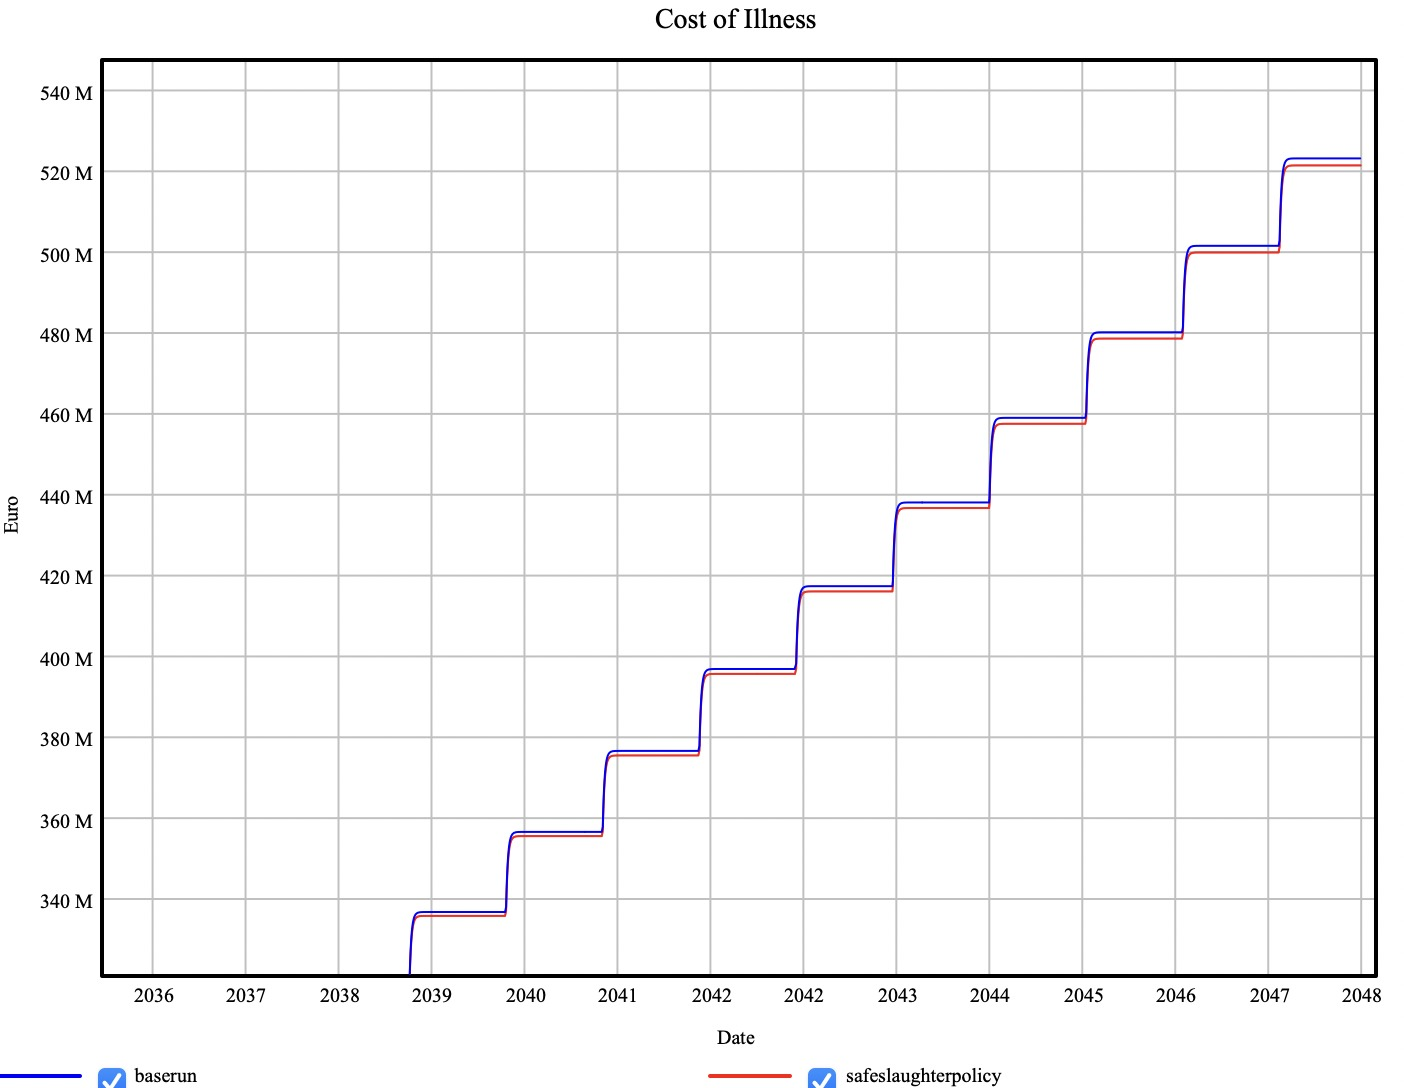
\includegraphics[width=1\textwidth]{images/p_coi.jpeg} 
        \caption{Cost of Illness in the Safe Slaughtering base run}
        \label{fig:p_coi}
    \end{minipage}\hfill
    \begin{minipage}{0.45\textwidth}
        \centering
        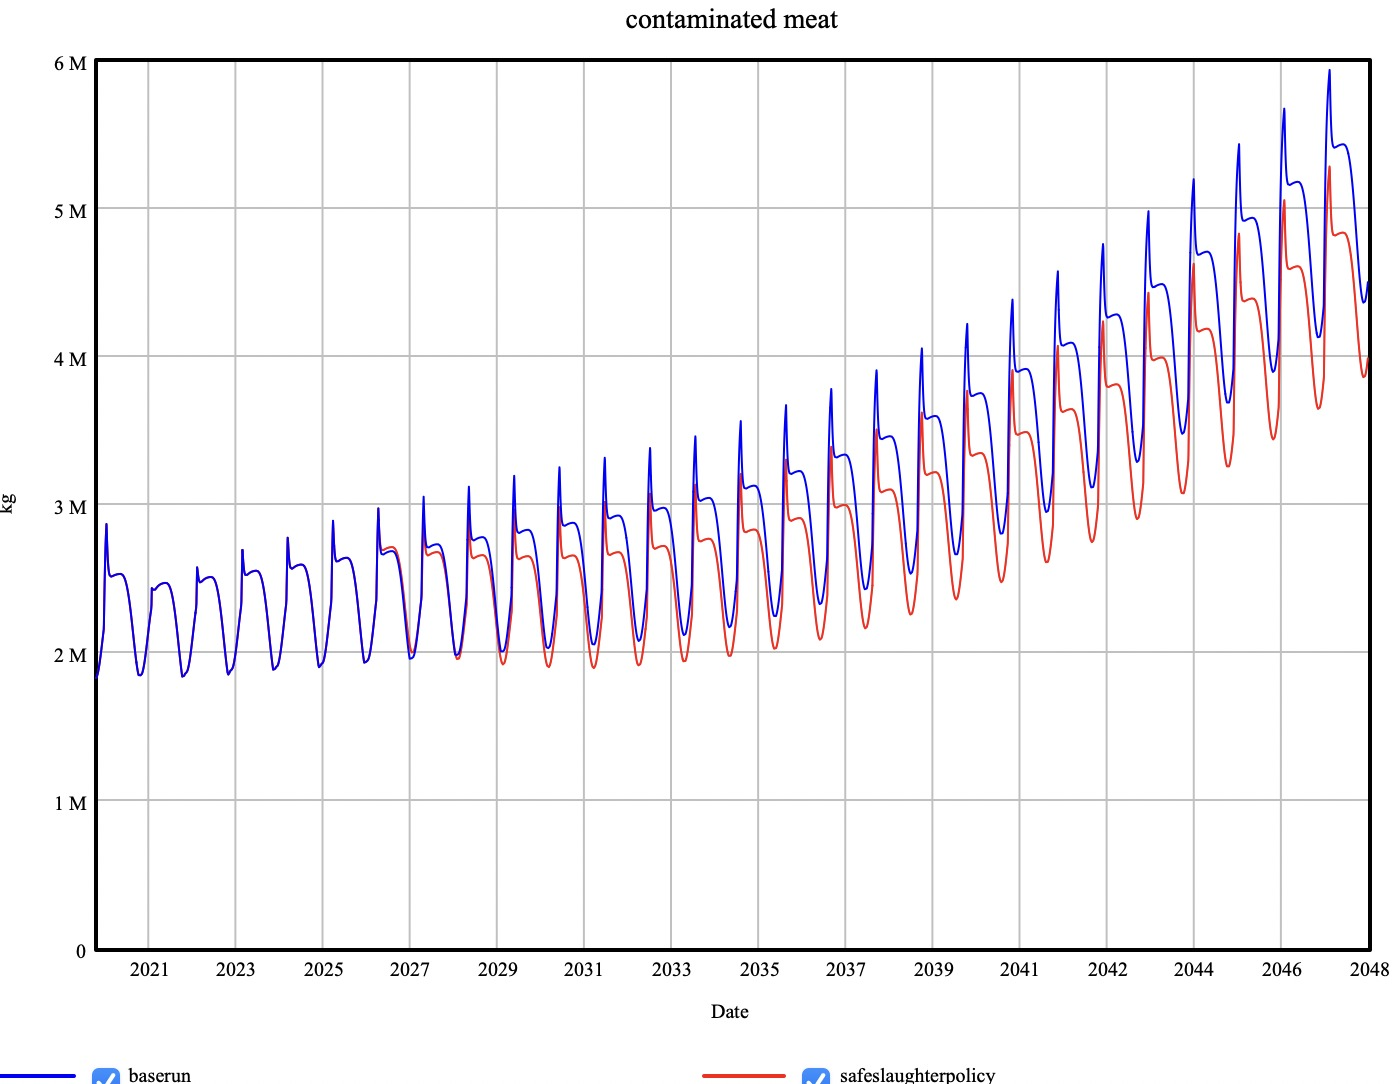
\includegraphics[width=1\textwidth]{images/p_meat.jpeg}
        \caption{Contaminated chicken meat in the Safe Slaughtering base run}
        \label{fig:p_meat}
    \end{minipage}
\end{figure} 

Model behaviour under this policy is reasonable. Once the food safety and handling policy goes into effect, the stock of contaminated meat decreases before slowly increasing again. This shows that it has an immediate effect, which stays over time but then continues growing. 

The odd spikes in Figure \ref{fig:p_meat} are similar to the ones as explained in section \ref{s:b_base}. 

Another policy implemented was the campaign to limit human exposure to flies, dubbed the No Fly Zone. This campaign would inform the Dutch population on how to minimise attractive environments for fly propagation. This policy reduces the rate of human exposure to infectious flies by 20\%. 

\begin{figure}[h!]
    \centering
    \begin{minipage}{0.45\textwidth}
        \centering
        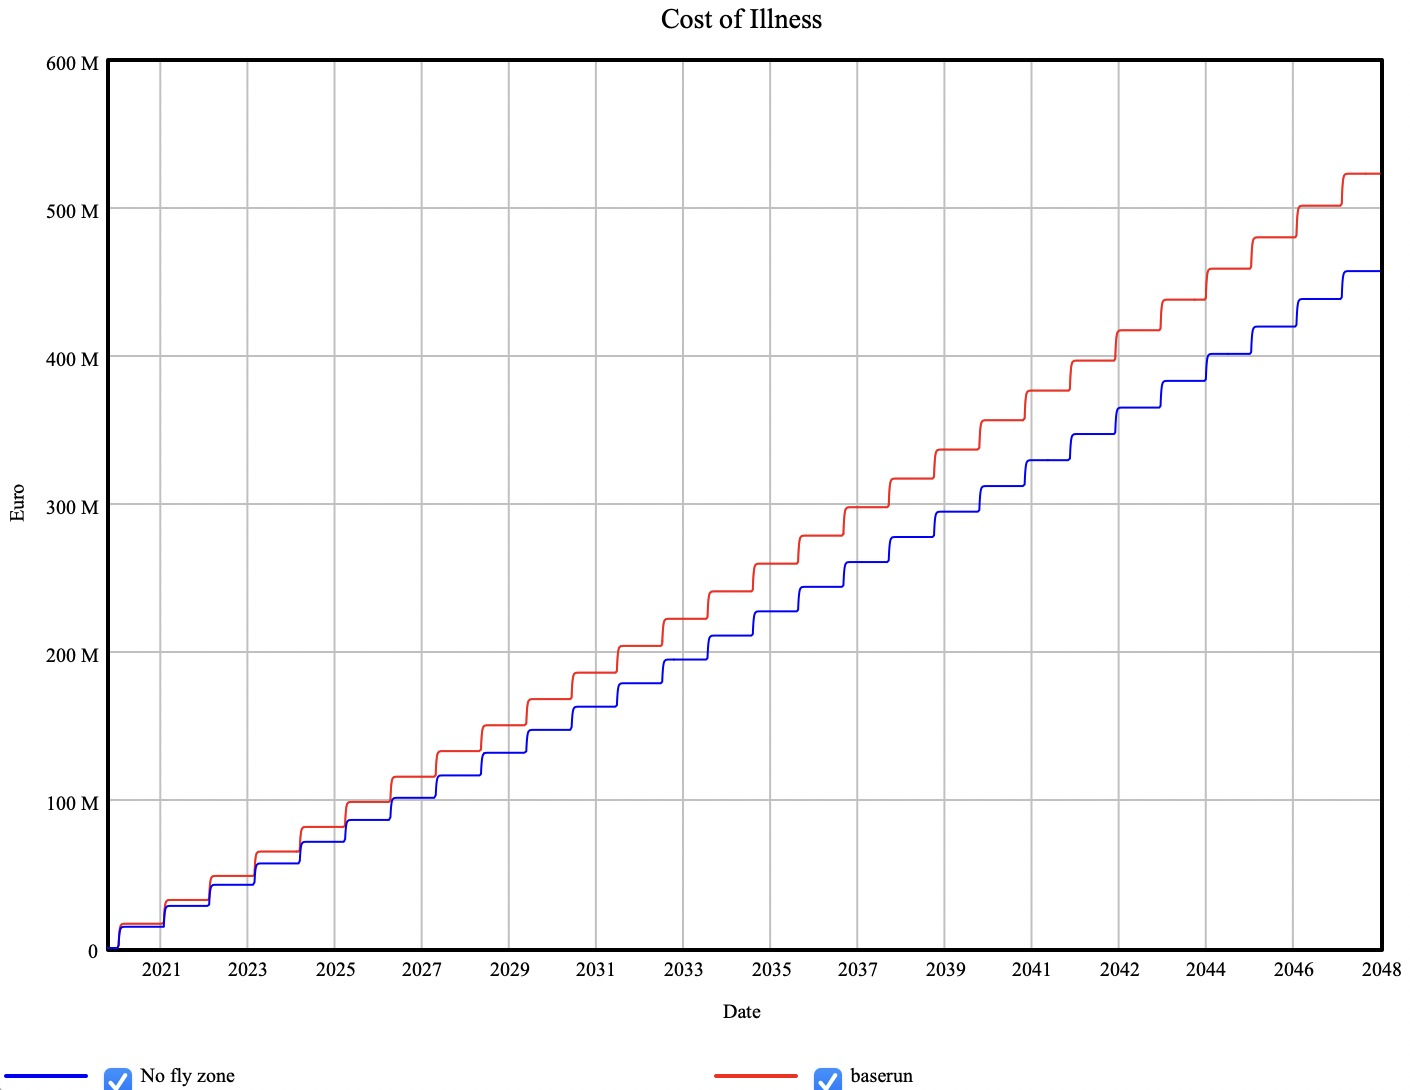
\includegraphics[width=1\textwidth]{images/p2_coi.jpeg} 
        \caption{Cost of Illness in the No Fly Zone base run}
        \label{fig:p2_coi}
    \end{minipage}\hfill
    \begin{minipage}{0.45\textwidth}
        \centering
        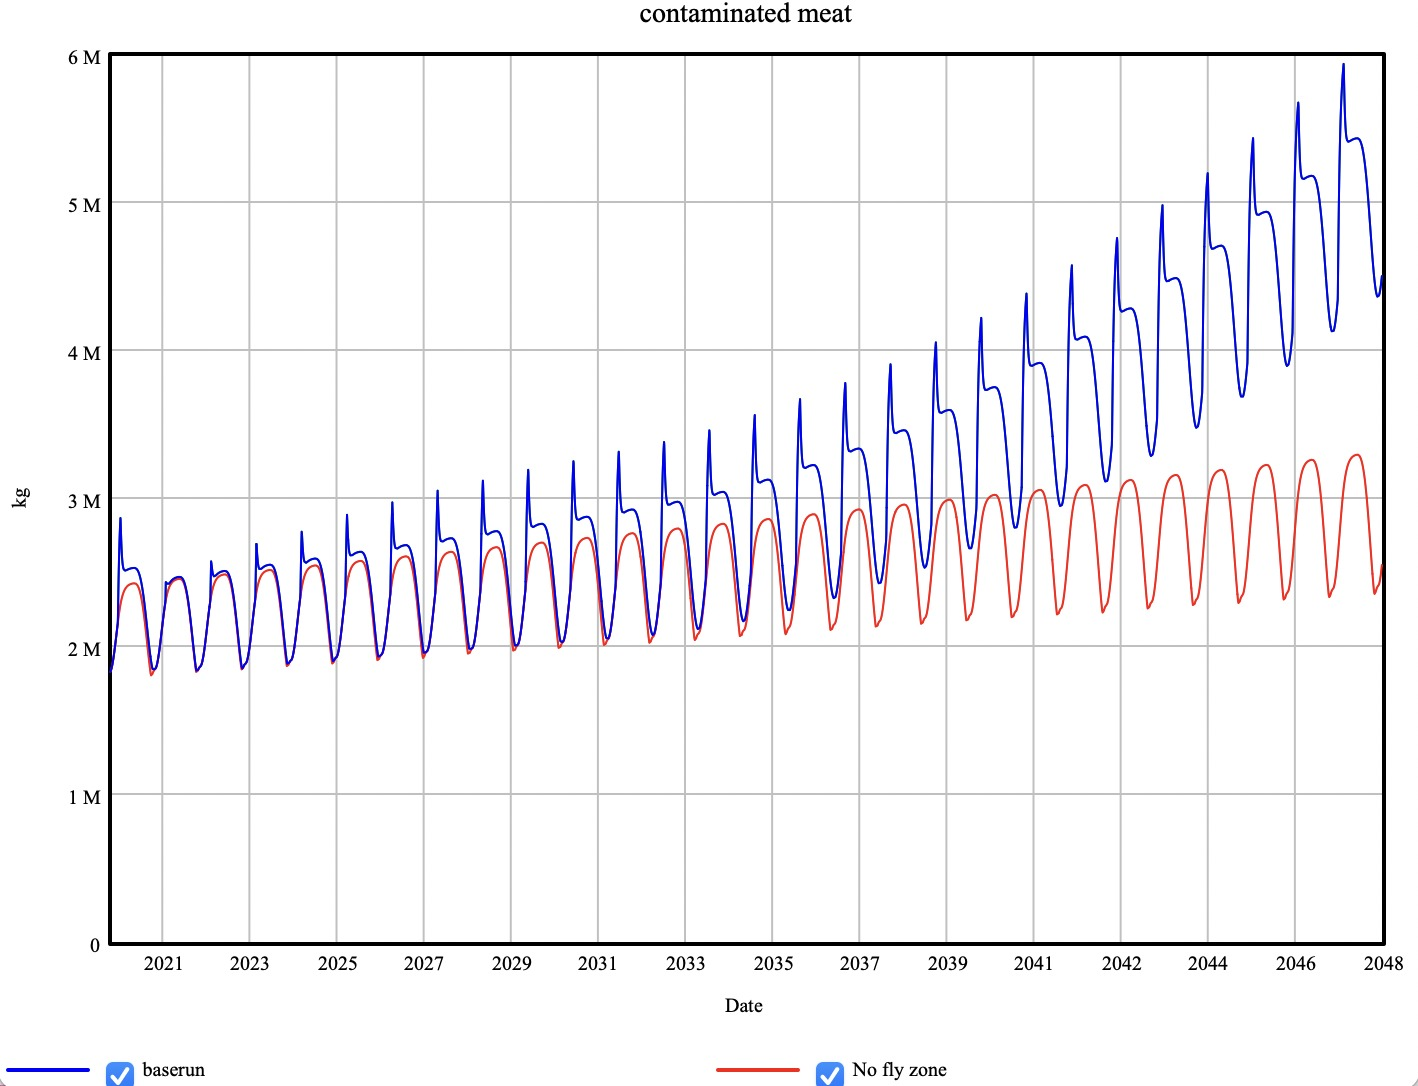
\includegraphics[width=1\textwidth]{images/p2_meat.jpeg}
        \caption{Contaminated chicken meat in the No Fly Zone base run}
        \label{fig:p2_meat}
    \end{minipage}
\end{figure} 

\begin{figure}[h]
\centering
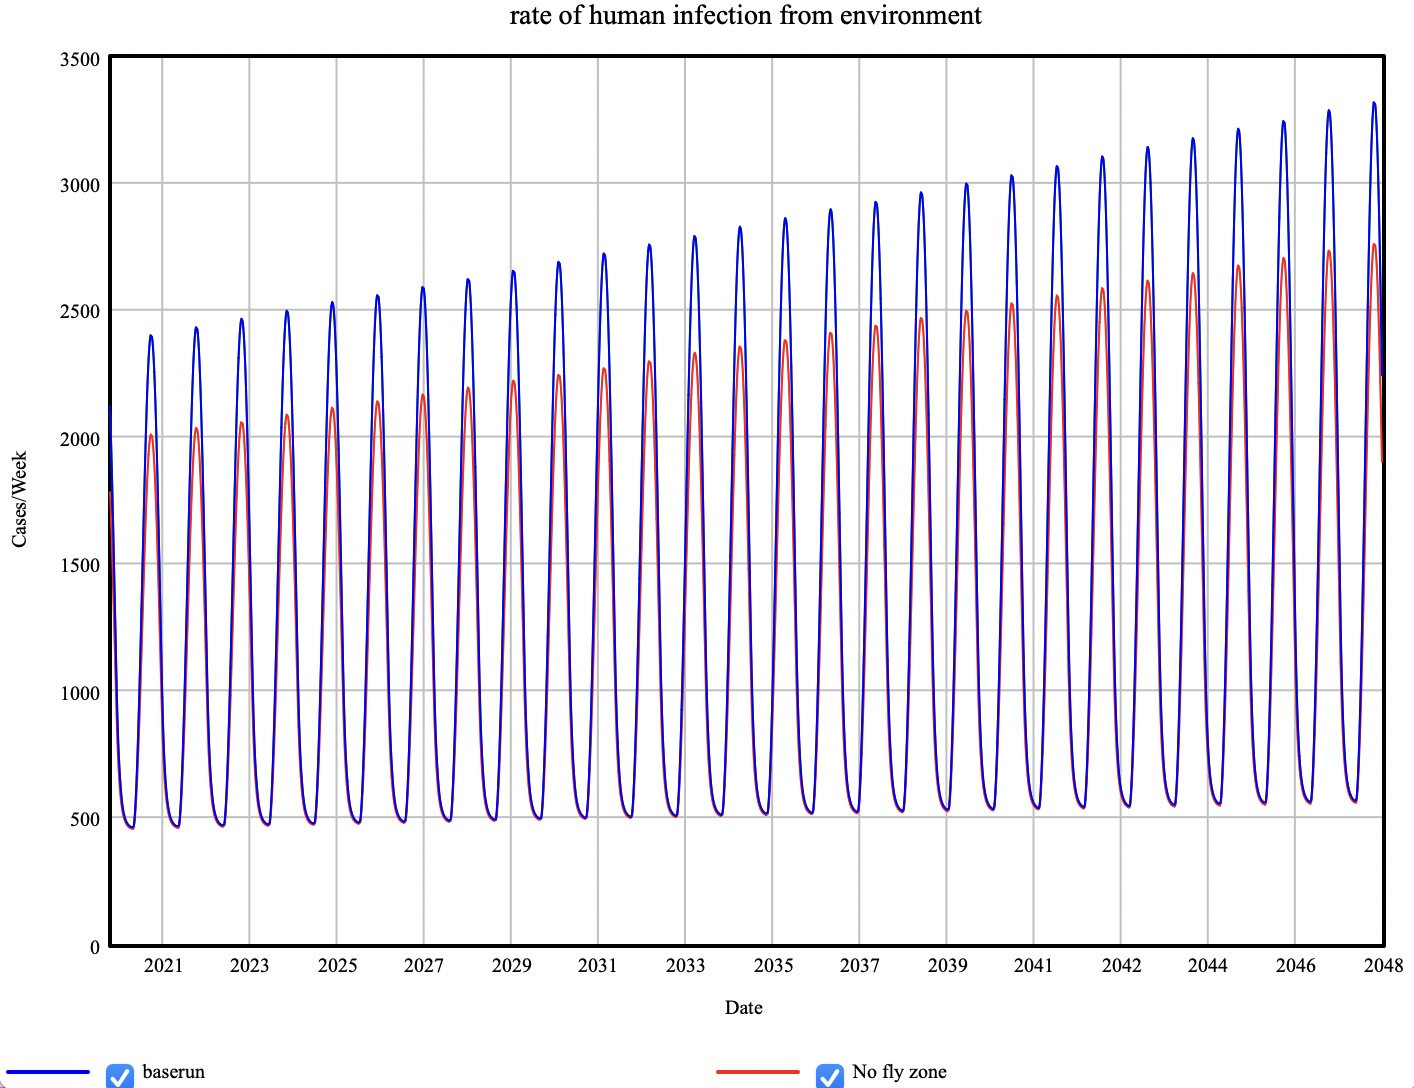
\includegraphics[width=0.45\textwidth]{images/p2_humanenvo.jpeg}
\caption{Human infections from the environment in the No Fly Zone base run }
\label{fig:p2_humanenvo}
\end{figure}

It can be seen in Figure \ref{fig:p2_meat} that the policy removes the strange peaks in the baserun. This is most likely due to the fact that the policy lowers the number of \textit{Campylobacter} cases, which mitigates the decrease of chicken meat consumption. This means that the threshold isn't met to trigger the meat consumption behaviour while the stock of contaminated meat decreases accordingly. 

Another fly related policy which was implemented is the the Pest Control policy. This Pest Control policy entails a policy that target the infectious flies and attempts to exterminate these fly populations in areas they would most likely be found, such as slaughterhouses and chicken farms.  

\begin{figure}[h!]
    \centering
    \begin{minipage}{0.45\textwidth}
        \centering
        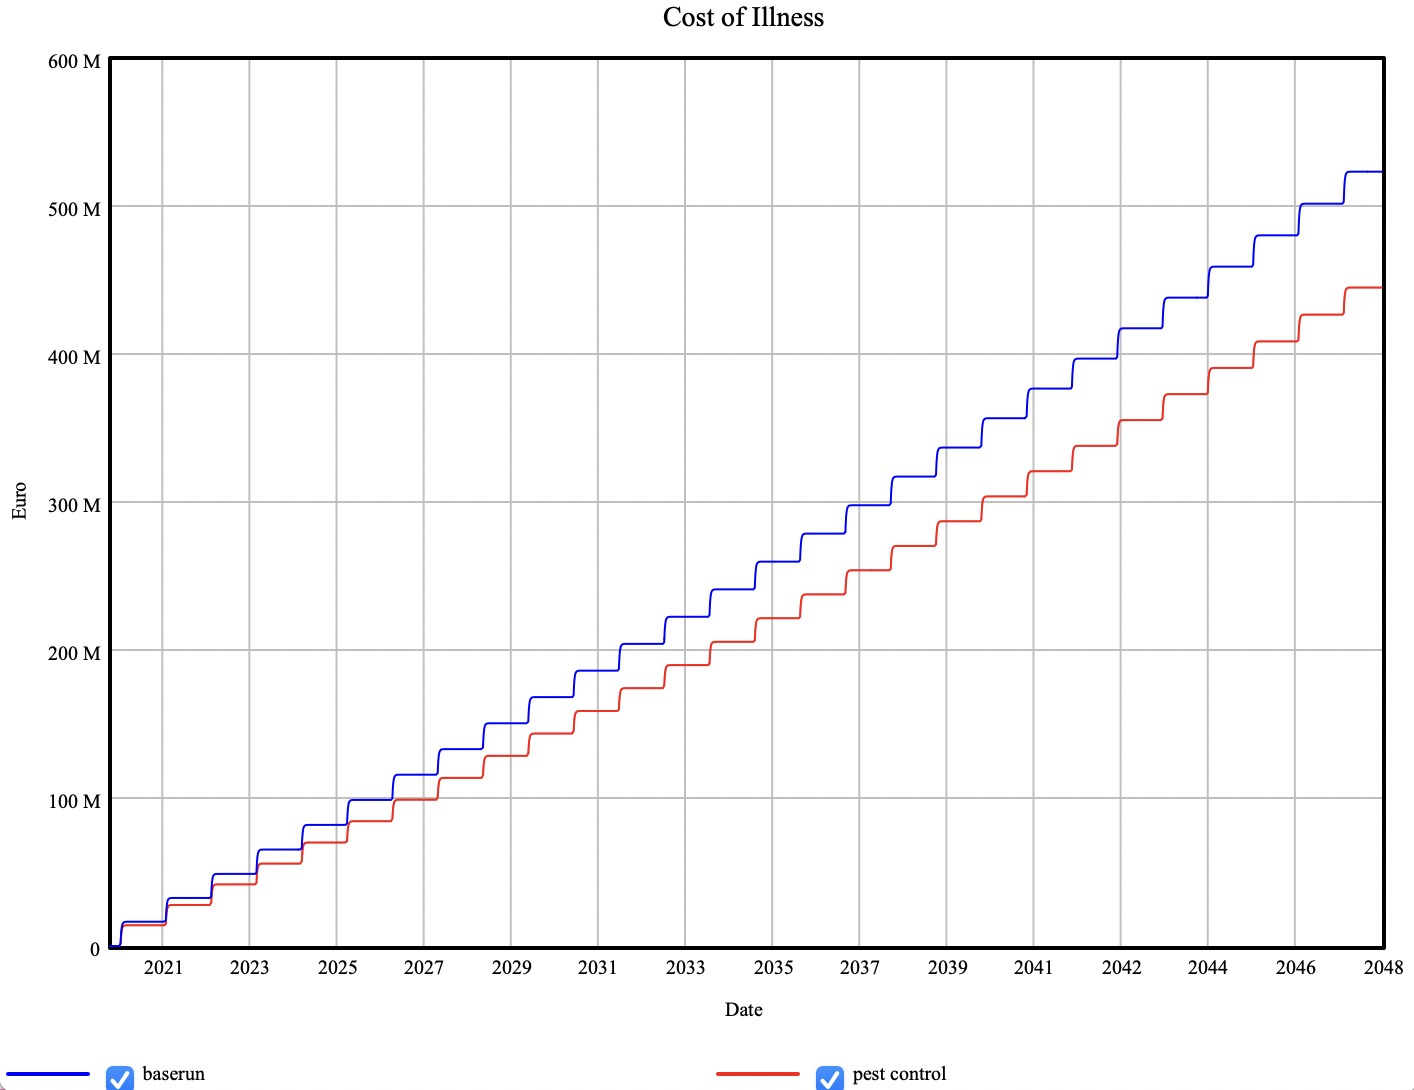
\includegraphics[width=1\textwidth]{images/p3_coi.jpeg} 
        \caption{Cost of Illness in the No Fly Zone base run}
        \label{fig:p3_coi}
    \end{minipage}\hfill
    \begin{minipage}{0.45\textwidth}
        \centering
        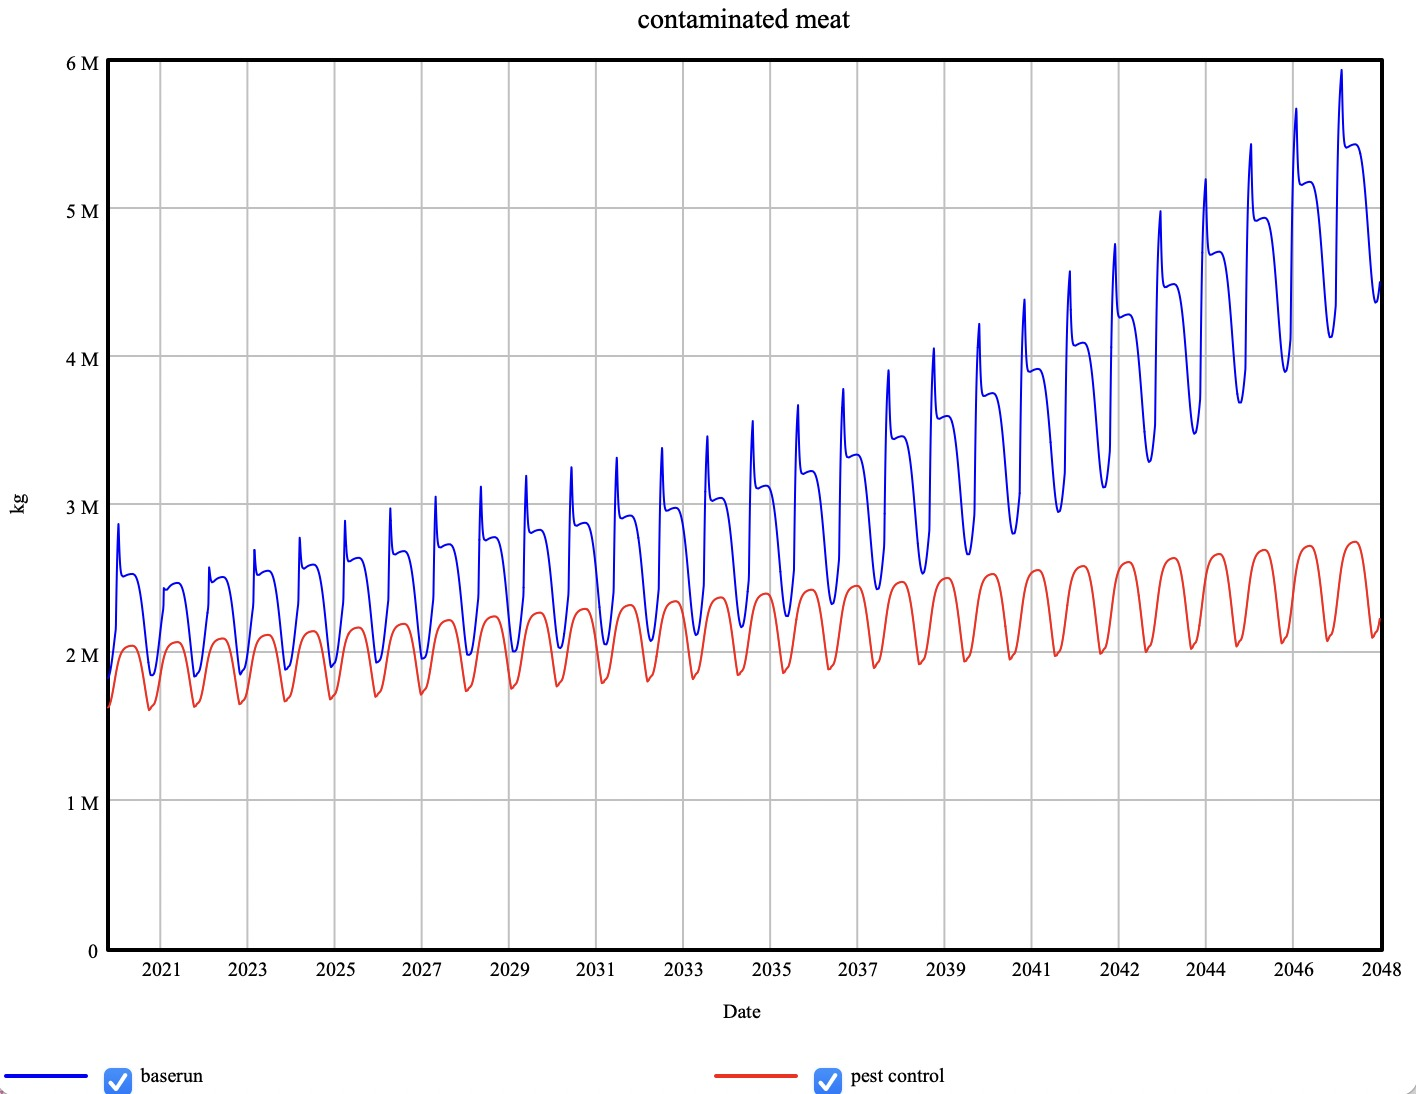
\includegraphics[width=1\textwidth]{images/p3_meat.jpeg}
        \caption{Contaminated chicken meat in the No Fly Zone base run}
        \label{fig:p3_meat}
    \end{minipage}
\end{figure} 

\begin{figure}[h!]
    \centering
    \begin{minipage}{0.45\textwidth}
        \centering
        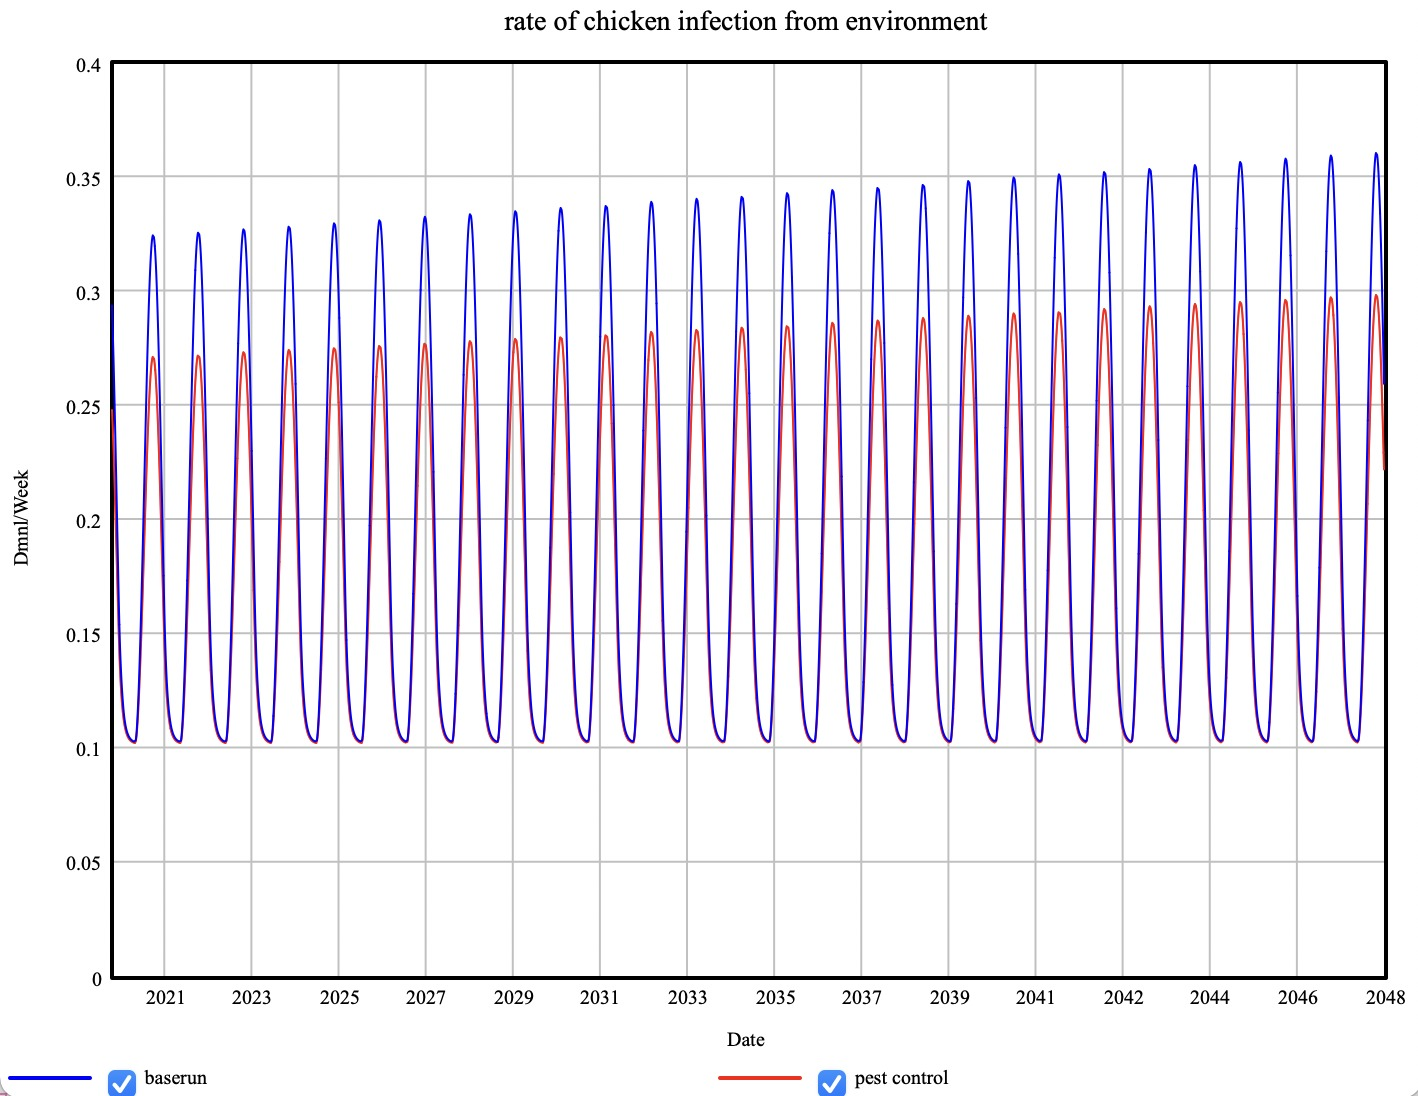
\includegraphics[width=1\textwidth]{images/p3_chicken.jpeg} 
        \caption{Chicken infections from the environment in the Pest Control base run}
        \label{fig:p3_chicken}
    \end{minipage}\hfill
    \begin{minipage}{0.45\textwidth}
        \centering
        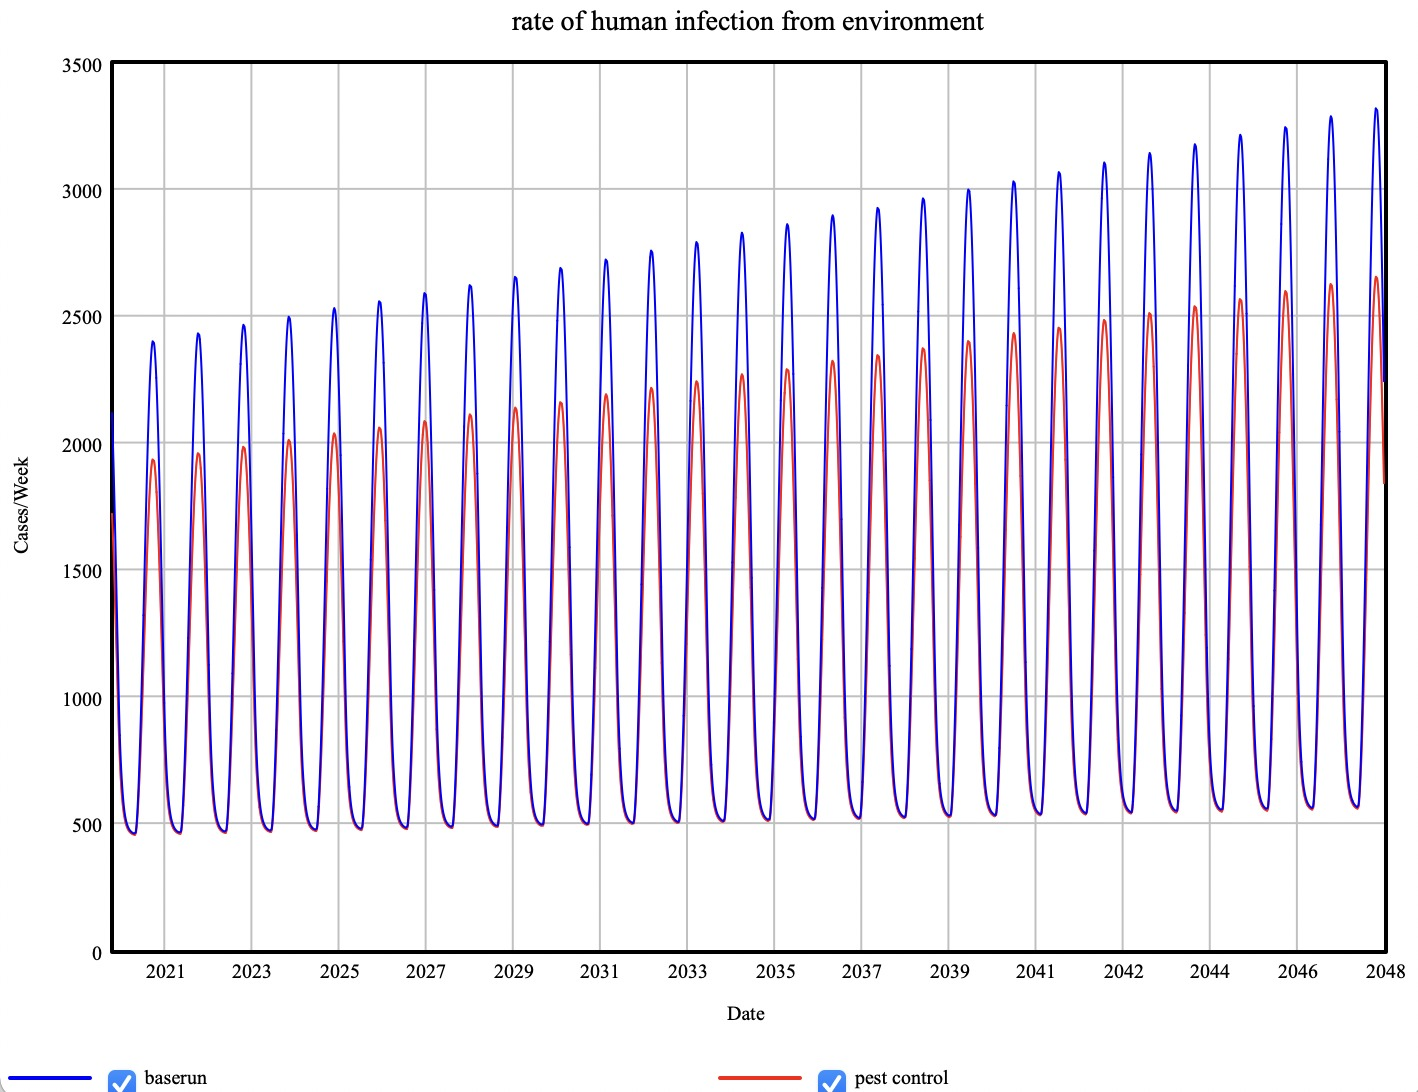
\includegraphics[width=1\textwidth]{images/p3_human.jpeg}
        \caption{Human infections from the environment in the Pest Control base run}
        \label{fig:p3_human}
    \end{minipage}
\end{figure} 

Two more policies regarding food were implemented, named food behaviour and preparation policies. Similar to the Safe Slaughtering policy, these policies go into effect when Cost of Illness reaches the 100 million threshold. These policies act on
\textit{consumption rate per person} and \textit{infections per kg of meat} respectively, by reducing these by 20\%.  

\begin{figure}[h!]
    \centering
    \begin{minipage}{0.45\textwidth}
        \centering
        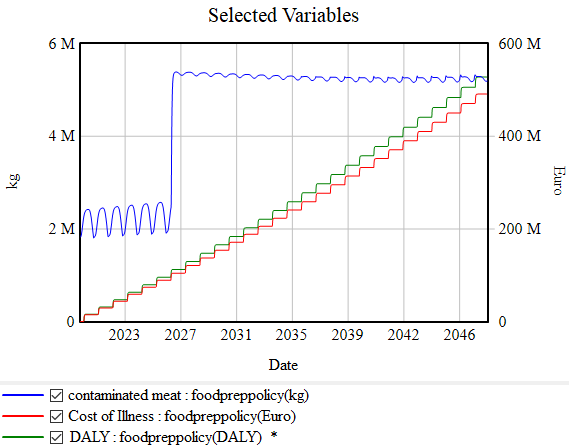
\includegraphics[width=1\textwidth]{images/foodbehaviourpolicy.png} 
        \caption{KPIs under food behaviour policy}
        \label{fig:foodbehav}
    \end{minipage}\hfill
    \begin{minipage}{0.45\textwidth}
        \centering
        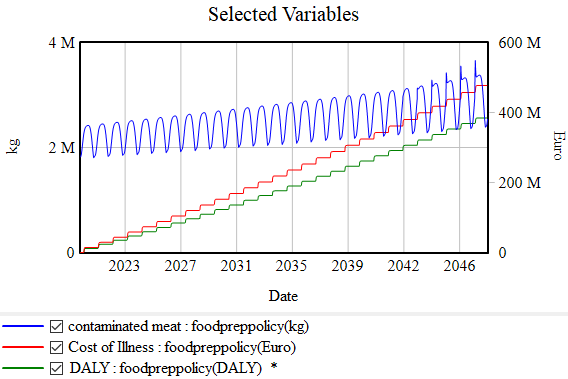
\includegraphics[width=1\textwidth]{images/foodpreparationpolicy.png}
        \caption{KPIs under food preparation policy}
        \label{fig:foodprep}
    \end{minipage}
\end{figure}

\fi

\subsection{Details on experiments}
\label{ch: detexp}
The policies employed in the model were tested against twelve scenarios, as detailed in Table \ref{tab:scenarios}. Scenarios 0, 1, 5 and 9 have the same values and are all baselines. The baseline simply contains a population increase that is also the medium increase, a temperature increase of 1.5 \degree c, a linear temperature change, and no rate of symptomatic cases modifier.

% Please add the following required packages to your document preamble:
% \usepackage{multirow}
\begin{table}[h!]
\caption{Scenarios under which the policies were tested for robustness}
\begin{tabular}{cl|lllll}
\hline
\multicolumn{1}{l}{}                                                           &                     &    & \multicolumn{4}{c}{Variable to change} \\ \cline{3-7} 
\multicolumn{2}{c|}{Test} &
  \multicolumn{1}{c}{\begin{tabular}[c]{@{}c@{}}Scenario\\ number\end{tabular}} &
  \multicolumn{1}{l}{\begin{tabular}[c]{@{}l@{}}Population \\ increase \\ by 2050\end{tabular}} &
  \multicolumn{1}{l}{\begin{tabular}[c]{@{}l@{}}Temperature \\ increase \\ by 2050\end{tabular}} &
  \begin{tabular}[c]{@{}l@{}}Temperature \\ switch\end{tabular} &
  \begin{tabular}[c]{@{}l@{}}Rate of \\ symptomatic \\ cases modifier\end{tabular} \\ \hline
\multicolumn{1}{l}{}                                                           & Baseline            & 0  & 1,94E+07     & 1.5     & 1    & 1      \\ \hline
\multirow{3}{*}{Population}                                                    & Medium increase     & 1  & 1.94E+07     & 1.5     & 1    & 1      \\
                                                                               & Large increase      & 2  & 2.16E+07     & 1.5     & 1    & 1      \\
                                                                               & Decrease            & 3  & 1.71E+07     & 1.5     & 1    & 1      \\ \hline
\multirow{3}{*}{\begin{tabular}[c]{@{}c@{}}Temperature \\ Change\end{tabular}} & 1 degree            & 4  & 1.94E+07     & 1       & 1    & 1      \\
                                                                               & 1.5 degree          & 5  & 19.4E+06     & 1.5     & 1    & 1      \\
                                                                               & 2 degree            & 6  & 19.4E+06     & 2       & 1    & 1      \\ \hline
\multirow{3}{*}{Seasonality}                                                   & No temp change      & 7  & 19.4E+06     & 1.5     & 0    & 1      \\
                                                                               & Fast temp change    & 8  & 19.4E+06     & 1.5     & 2    & 1      \\
                                                                               & Linear temp change  & 9  & 19.4E+06     & 1.5     & 1    & 1      \\ \hline
\multirow{2}{*}{\begin{tabular}[c]{@{}c@{}}Public \\ Health\end{tabular}}      & 10\% fewer symptoms & 10 & 19.4E+06     & 1.5     & 1    & 0.9    \\
                                                                               & 10\% more symptoms  & 11 & 19.4E+06     & 1.5     & 1    & 1.1    \\ \hline
\multicolumn{1}{l}{}                                                           & Worst case          & 12 & 2.16E+07     & 2       & 2    & 1.1   
\end{tabular}
\label{tab:scenarios}
\end{table}

%TC:endignore
\clearpage
\section{Report log}
\label{ch:report_log}
The working hours of each member of this group were logged, and they are shown in their respective subsections.
\subsection{Elias Bach}
Elias was a member of this group and his contributions are shown in Table~\ref{tab:elias_log}. 
\begin{longtable}[c]{c|c|m{35em}}
\caption{Elias' report log}
\label{tab:elias_log}\\
\textbf{Date}& \textbf{Hours} & \textbf{Task} \\
\hline
\endfirsthead
%
\endhead
%
09-02 & 1.5 & Meeting with group, create bull's-eye diagram and write notes on scope\\
10-02 & 1 & Meeting with group \\
11-02 & 1.5 & Reviewed and improved the answer to question 4 of assignment 1, made an SSD diagram draft \\
12-02 & 1 & Meeting with team and divided tasks for Sunday\\ 
12-02 & 0.5 & figured out how to work with submodels and views in Vensim \\
12-02 & 2 & Recreated submodels 1 and 3 in Vensim
17-02 & 0.5 & Began part of introduction for assignment 2
18-02 & 1 & Continued part of introduction for assignment 2

\end{longtable}
%TC:ignore

% Please add the following required packages to your document preamble:
% \usepackage{longtable}
% Note: It may be necessary to compile the document several times to get a multi-page table to line up properly
\subsection{David Matheus}
David's contributions are shown in Table~\ref{tab:david_log}. 
\begin{longtable}[c]{c|c|m{35em}}
\caption{David's report log}
\label{tab:david_log}\\
\textbf{Date}& \textbf{Hours} & \textbf{Task} \\
\hline
\endfirsthead
%
\endhead
%
09-02   &   1.5     &   Team meeting, drafted model purpose.                                         \\
10-02   &   1       &   Team meeting, reviewed work.                                                 \\
11-02   &   0.5     &   Drafted conceptual model about fly infection loop.                           \\
12-02   &   1       &   Team meeting, divided tasks for Sunday.                                      \\
16-02   &   0.75    &   Team meeting, reviewed assignment 1 and divided tasks.                       \\
18-02   &   1       &   Team meeting, reevaluation of model aggregation.                             \\
18-02   &   2.5     &   Meeting with Menghua, stocks and flows model.                                \\
18-02   &   0.5     &   Work on stocks and flows model.                                              \\
19-02   &   1       &   Team meeting, discussed changes to conceptualisation and stocks and flows.   \\
19-02   &   0.75    &   Work on stocks and flows model.                                              \\
19-02   &   1       &   Meeting with Menghua, stocks and flows model.                                \\
23-02   &   1       &   Meeting with group, divided tasks for the week.                              \\
24-02   &   0.5     &   Work on chicken infection sub-model.                                         \\
25-02   &   1.5     &   Group meeting, discussed models and sub-models, assigned tasks.              \\
25-02   &   1.5     &   Work on chicken infection sub-model and report writing.                      \\
26-02   &   0.5     &   Group meeting, review for submission.                                        \\
27-02   &   0.5     &   Peer review group 9b's work.                                                 \\
28-02   &   0.5     &   Peer review.                                                                 \\
04-03   &   1       &   Meeting with group.                                                          \\
08-03   &   0.25    &   Updated Lisette on project.                                                  \\
09-03   &   1.5     &   Worked on conceptualisation for chicken contamination part of general model. \\
11-03   &   4.5     &   Worked on general model with the group in Wijnhaven.                         \\
12-03   &   1       &   Worked on conceptualisation for general model.                               \\
18-03   &   6.5     &   Worked on model with the group at Wijnhaven.                                 \\
24-03   &   2.5     &   Brief team meetings, worked on model and report writing.                     \\
25-03   &   1.5     &   Meeting, experimental design, remade chicken CLD and wrote report.           \\
26-03   &   6       &   Meeting with the group at Wijnhaven, experiment setup, sensitivity analysis. \\
29-03   &   0.5     &   Group meeting.                                                               \\
31-03   &   1       &   Group meeting, divided tasks and prepared presentation.                      \\
01-04   &   1       &   Presentation and group meeting.                                              \\
02-04   &   1       &   Reran sensitivity analysis, prepared consumption behaviour experiment.        \\
04-04   &   2.5     &   Corrected errors, reconceptualised behaviour experiment, reran experiment.    \\
05-04   &   2.5     &   Detailed revision of model and documentation.                                \\
06-04   &   3       &   Group meeting, more revision, data export.                                   \\
07-04   &   6       &   Meeting at Wijnhaven, results discussion, extreme conditions, report writing.\\
08-04   &   3.5     &   Brief group meeting, report writing and reviewing.                           \\
09-04   &   1.5     &   Meeting with group, last details. \\



\end{longtable}

%TC:endignore
%TC:ignore

\subsection{Menghua Prisse}
Menghua was a member of this group and her contributions are shown in Table~\ref{tab:menghua_log}. 
\begin{longtable}[c]{c|c|m{35em}}
\caption{Menghua's report log}
\label{tab:menghua_log}\\
\textbf{Date}& \textbf{Hours} & \textbf{Task} \\
\hline
\endfirsthead
%
\endhead
%
09-02  & 1.5 & Meeting with group, drafted dynamic hypothesis and synthesized with Lisette's solution\\
10-02 & 1 & Meeting with group \\ 
11-02 & 1.5 & Reviewed and worked on Question 2 of Assignment 1 \\
14-02 & 1 & Reviewed adjustments to Assignment 1 \& started for Assignment 2 \\ 
16-02 & 0.75 & Meeting with group \\ 
17-02 & 0.25 & Presentation prep \\
18-02 & 3.5 & Meeting with group and working on the Stock Flow diagram with David  \\
19-02 & 2 & Meeting with group and working on the Stock Flow diagram with David \\ 
21-02 & 1 & Go over what has been written already to become familiar with it \\
24-02 & 1 & Read up on sewage systems \\ 
25-02 & 1.5 & Read over text \\ 
26-02 & 1.5 & Meeting with group and going over Introduction and peer review of group 9b \\ 
01-03 & 1 & Peer review of group 9b \\
04-03 & 1 & Meeting with group \\
07-03 & 1 & Read into new sources and worked on conceptualisation for the general model \\ 
10-03 & 1 & Continued work on conceptualisation and discussed COI with Emily \\ 
11-03 & 4.5 & Worked on the model with the group \\
18-03 & 6.5 & Worked on the model with the group \\
13-03 & 1 & Studied changes to model \\ 
24-03 & 2 & Discussed how to continue with the report (morning) and worked on model verification (afternoon) \\ 
25-03 & 4 & Worked on model verification, adjusted dynamic hypothesis and helped Lisette (not all hours were productive) \\ 
26-03 & 6 & Adjustments to model and worked on the report \\ 
30-03 & 0.5 & Going over peer review \\
31-03 & 1 & Split tasks and made presentation \\
01-04 & 1.5 & Presentation and group meeting and planned own tasks \\ 





\end{longtable}

%TC:endignore
%TC:ignore

% Please add the following required packages to your document preamble:
% \usepackage{longtable}
% Note: It may be necessary to compile the document several times to get a multi-page table to line up properly
\subsection{Emily Ryan}
Emily was a member of this group and her contributions are shown in Table~\ref{tab:emily_log}. 
\begin{longtable}[c]{c|c|m{35em}}
\caption{Emily's report log}
\label{tab:emily_log}\\
\textbf{Date}& \textbf{Hours} & \textbf{Task} \\
\hline
\endfirsthead
%
\endhead
%
 09-02  &   1.5    & Meeting with group and draft subsystem diagram  \\
 10-02  &    1   & Meeting with group  \\
 12-02  &    1.5   & Meeting with group and draft KPIs/dynamic hypothesis  \\
 14-02  & 2.5  & Final editing and write-up for Assignment 1\\
 16-02 & 1 & Meeting with group and planning work\\
 17-02 & 0.5 & Presentation slides for first review\\
 18-02 & 2 & Team meeting, presentation and report writing\\
 19-02 & 2 & Team meeting and report writing\\
 21-02 & 2 & Report writing\\
 23-02 & 3 & Team meeting and conceptualising COI sub-model\\
 25-02 & 3 & Report writing and Team meeting\\
 26-02 & 1.5 & Finalise COI text, update dynamic hypothesis and team meeting\\
 04-03 & 4 & Team meeting and identifying values for COI submodel\\
 05-03 & 1 & Research and further conceptualisation COI and disease burden submodels\\
 09-03 & 2 & Research and valuation for COI submodel and update Lisette\\
 10-03 & 1.5 & Reconceptualise COI and disease burden model for model-building \\
 11-03 &  4.5 & Working on model with the group \\
 15-03 & 1.5 & Report writing \\
 18-03 & 6.5  & Working on model with the group \\
 20-03 & 1 & Worked on the model with Elias and Lisette and discussed structural uncertainty \\
 21-03 & 1 & Group meeting with Lisette and Elias\\
 23-03 & 2 & Report writing\\
 24-03 & 1 & Meeting with group and report writing\\
 25-03 & 2 & Meeting with group and report writing\\
 26-03 & 7 & Meeting with group - report writing and modelling\\
 29-03 & 1 & Meeting with group and group 9b review\\
 30-03 & 1 & Review group 9b and prepare task list\\
 31-03 & 0.5 & Finalise final task list for group\\
 

\end{longtable}

%TC:endignore
%TC:ignore
% ̿' ̿'\̵͇̿̿\з=(◕_◕)=ε/̵͇̿̿/'̿'̿ ̿
\subsection{Lisette de Schipper}
Lisette was a member of this group and her contributions are shown in Table~\ref{tab:lisette_log}. 
\begin{longtable}[c]{c|c|m{35em}}
\caption{Lisette's report log}
\label{tab:lisette_log}\\
\textbf{Date}& \textbf{Hours} & \textbf{Task} \\
\hline
\endfirsthead
%
\endhead
%
08-02 & 1 & Set up Zotero, Github and Overleaf \\
09-02 & 1.5 & Meeting with group, created dynamic hypothesis and sketched expected behaviour of KPIs\\
10-02 & 1 & Meeting with group \\
11-02 & 1 & Reviewed and improved the answer to question 1 of assignment 1 \\
12-02 & 1.5 & Meeting with team and divided tasks for Sunday, figured out how to work with submodels and views in Vensim \\
13-02 & 0.5 & Recreated submodels 2 and 4 in Vensim \\
16-02 & 0.75 & Meeting with group, collectively reviewed assignment 1, and divided tasks \\
18-02 & 2.5 & Meeting with group, attended presentation for Jill and Irene, reflected with group on feedback, gave tutorials on Zotero, and started working on introduction, improved dynamic hypothesis \\
19-02 & 1.5 & Meeting with group, discussed dynamic hypothesis \& conceptualisation, worked on introduction, included glossary \\
20-02 & 0.75 & Continued working on introduction \\
23-02 & 1.5 & Continued working on introduction and meeting with group \\
24-02 & 2 & Started construction + research of the environmental submodel \\
25-02 & 3 & Meeting with group and continued working on environmental submodel \\
26-02 & 1.5 & Continued working on environmental model and meeting with group \\
27-02 & 1 & Worked on peer review of group 9b \\
28-02 & 1.5 & Worked on peer review of group 9b \\
08-03 & 0.25 & Got updates on project from David \\
09-03 & 0.5 & Got updates on project from Emily \\
10-03 & 2 & Worked on environmental submodel with Elias \\
11-03 & 4 & Worked on the model with the group \\
18-03 & 4  & Worked on the model with the group \\
20-03 & 1 & Worked on the model with Elias and Emily and discussed structural uncertainty \\
23-03 & 0.5 & Worked on model and on report \\
24-03 & 1.5 & Met with group and worked on validation 
\end{longtable}

%TC:endignore
%TC:endignore

\end{document}          
